\PassOptionsToPackage{numbers}{natbib}
\documentclass[ppgc,diss,english]{iiufrgs}

\usepackage[T1]{fontenc}        % pacote para conj. de caracteres correto
%\usepackage[latin1]{inputenc}   % pacote para acentuao
\usepackage{times}              % pacote para usar fonte Adobe Times

% graphics
\usepackage{graphicx}
\usepackage{epstopdf}

% math
\usepackage{amsmath}

\usepackage{url}

% table
\usepackage{multirow}
\usepackage{longtable}
\usepackage{array}
\usepackage{rotating}

\usepackage{subfigure}

\usepackage[alf,abnt-emphasize=bf]{abntex2cite}	% pacote para usar citações abnt

% General Information
\title{A Benchmark Suite for Distributed Stream Processing Systems}
\author{Bordin}{Maycon Viana}
\advisor[Prof.~Dr.]{Geyer}{Claudio Fernando Resin}
%\date{maio}{2001}
%\course{Pós-Grad}
\location{Porto Alegre}{RS}

% keywords
\keyword{distributed systems}
\keyword{benchmark suite}
\keyword{stream processing}
\keyword{real-time processing}
\keyword{big data}

\begin{document}

% title page
\maketitle

% summary
\tableofcontents

% list of abbreviations
\begin{listofabbrv}{SPMD}
        \item[SMP] Symmetric Multi-Processor
        \item[NUMA] Non-Uniform Memory Access
        \item[SIMD] Single Instruction Multiple Data
        \item[SPMD] Single Program Multiple Data
        \item[ABNT] Associação Brasileira de Normas Técnicas
        
        
        \item[SPS] Stream Processing System
        \item[SPA] Stream Processing Application
        \item[SPE] Stream Processing Engine
        \item[ESP] Event-Stream Processing
        \item[DSMS] Data Stream Management System
        \item[CEP] Complex Event Processing
        \item[IFP] Information Flow Processing
        \item[CQ] Continuous Query
        \item[PE] Processing Element
        \item[ECA] Event-Condition-Action
        \item[SQL] Structured Query Language
        \item[DBMS] Data Base Management System
        \item[ETL] Extract/Transform/Load
        
        \item[DSL] Domain Specific Language
        
        \item[VWAP] Volume-Weighted Average Price
        \item[TAQ] Trade And Quote
        
\end{listofabbrv}

% list of figures
\listoffigures

% list of tables
%\listoftables

% abstract
\begin{abstract}
Recently a new application domain characterized by the continuous and low-latency processing of large volumes of data has been gaining attention. The growing number of applications of such genre has led to the creation of \emph{Stream Processing Systems} (SPSs), systems that abstract the details of real-time applications from the developer. More recently, the ever increasing volumes of data to be processed gave rise to distributed SPSs. Currently there are in the market several distributed SPSs, however the existing benchmarks designed for the evaluation this kind of system covers only a few applications and workloads, while these systems have a much wider set of applications. In this work a benchmark for stream processing systems is proposed. Based on a survey of several papers with real-time and stream applications, the most used applications and areas were outlined, as well as the most used metrics in the performance evaluation of such applications. With these information the metrics of the benchmark were selected as well as a list of possible application to be part of the benchmark. Those passed through a workload characterization in order to select a diverse set of applications. To ease the evaluation of SPSs a framework was created with an API to generalize the application development and collect metrics, with the possibility of extending it to support other platforms in the future. To prove the usefulness of the benchmark, a subset of the applications were executed on Storm and Spark using the Azure Platform and the results have demonstrated the usefulness of the benchmark suite in comparing these systems.
\end{abstract}


% -----------------------------------------------------------------------------
\chapter{Introduction}

% overview of the current scenario
% motivation for the work and problems to solve
% main goal and specific goals
% main contributions of the work
% organization of the rest of the document

A data by itself holds no value unless it has been interpreted, contextualized and aggregated with other data, then it has a value, which makes of it an information. In some classes of applications the value is not only on the information, but also on the speed with which it's obtained. High Frequency Trading (HFT) is a great example of applications where the profitability is directly proportional to the latency \cite{Loveless:2013:OAH:2507771.2507780}. With the evolution of hardware and data processing tools many applications that in the past took hours to give a response to a query, now need to answer in a matter of minutes or seconds \cite{barlow2013real}. 

This kind of application has as a characteristic, beyond the need for real-time or near real-time processing, the continuous ingestion of large and unbounded volumes of data in the shape of tuples or events. The growing demand for applications that would meet these requirements led to the creation of systems that provide a programming model that take away from the programmer the responsibility with respect to details such as scheduling, fault tolerance, processing and optimization of queries. These systems are know as Stream Processing Systems (SPS), Data Stream Management Systems (DSMS) \cite{chakravarthy2009stream} or Stream Processing Engines (SPE) \cite{abadi2005design}.

Lately these systems adopted a distributed architecture as a way to deal with ever increasing volumes of data \cite{zaharia2012discretized}. Among them are S4, Storm, Spark Streaming, Flink Streaming and more recently Samza and Apache Beam.

These systems model the data processing through a data flow graph with the vertices being the operators and the edges the data streams. But the similarities don't go much further, as each of these systems has different mechanisms for fault tolerance and recovery, scheduling and parallelism of operators, and communication patterns.

In this scenario it would be useful to have a tool for comparing these systems under different workloads, to assist in the selection of the most suited for a specific job. We propose a benchmark suite composed of applications from different fields of applications, as well as a methodology for evaluating distributed SPSs.

\section{Motivation}

Recently a new application domain characterized by the continuous and low-latency processing of large volumes of data has been gaining attention. The growing number of applications of such genre has led to the creation of \emph{Stream Processing Systems} (SPSs), systems that abstract details that have no direct relation to the problem at hand.

More recently, the ever increasing volumes of data to be processed gave rise to distributed SPSs. Currently there are in the market several distributed SPSs, however the benchmarks that currently exist for these systems use only synthetic, very simple applications or only applications from a few areas.

\section{Goals}

The main goal of this work is the creation of a benchmark suite for SPSs composed of applications from different areas, workloads and data loads, defining metrics for the measurement of the performance, scalability and reliability, and scenarios with the occurrence of failures and bursts in the volume of data. With this benchmark suite we expect to provide a reference point so that people interested in using an SPS can choose the one that better fits its needs.

The second goal is to apply the benchmark suite in a comparison between the main distributed SPSs in the market. Through this comparison we expect to demonstrate the usefulness of this benchmark suite, as well as provide a reference implementation of the benchmark so that it can be applied in other SPSs.

\section{Contributions}

This research work expects to contribute with:

\begin{itemize}
\item \textbf{Define a solid set of metrics for stream processing}.\\
	  This work aims to research all previous works, gather information on all metrics used and then define the ones that are better suited for evaluating SPSs.

\item \textbf{Become a standard on SPS benchmarking}.\\
      Or at least improve the way these systems are evaluated, with higher quality benchmarks that can better show how they perform in different scenarios.
      
\item \textbf{Provide a defined set of applications for benchmarking}.\\
      As well as a reference implementation for those applications, so that they can be reproduced in other SPSs.
      

\end{itemize}


\section{Document Organization}

After this first Chapter, which contains a brief introduction of this research, the rest of this document is organized as follows:

Chapter \ref{chapter:event-stream-processing} introduces the basic concepts of Stream Processing on Sections \ref{sec:esp:requirements} and \ref{sec:esp:concepts}. On Section \ref{sec:esp:history} the history of Stream Processing and what came before it is described. Then it moves to more specific areas of Stream Processing, such as operator placement on Section \ref{sec:esp:scheduling_load_balancing}, fault tolerance on Section\ref{sec:esp:fault_tolerance} and message systems on Section \ref{sec:esp:data_transport}. We introduce the main platforms of stream processing on Section \ref{sec:esp:platforms} and then the main work done in performance evaluation of these platforms on Section \ref{sec:esp:performance_evaluation}.

On Chapter \ref{chapter:model} the model of this research is described, detailing the methodology for benchmarking SPSs on Section \ref{sec:methodology}, including the metrics that are going to be used for evaluation of these systems. On Section \ref{sec:application-selection} we describe how the selection of applications took place and then on Section \ref{sec:applications} we describe these applications in detail. In the end, at Section \ref{sec:workload-characterization}, a workload characterization of these applications is described and finally the configurations and datasets that can be used to execute these applications, on Section \ref{sec:configuration_datasets}.

The results of the performance evaluation of Storm and Spark using a subset of the applications of the benchmark are on Chapter \ref{chapter:results}. In Section \ref{sec:set-up} the set-up of the environment is described, and in the subsequent sections the results in each application evaluated are shown.

At last, in Chapter \ref{chapter:conclusion}, are the conclusions of this research as well as the final considerations and future work.

% -----------------------------------------------------------------------------
\chapter{Event-Stream Processing}
\label{chapter:event-stream-processing}

%This chapter introduces the concepts that govern Stream Processing Systems (SPSs), also known as Event-Stream Processing (ESP) or Stream Processing Engines (SPEs), in Section \ref{sec:esp:concepts}. Section \ref{sec:esp:history} traces the history of SPSs back to the first Data Stream Management Systems (DSMSs), Complex Event Processing systems (CEPs), Continuous Queries and Active Databases.
%
%In sequence, the architectural aspects of SPSs are explored, including tecniques for scheduling and load balancing jobs and tasks within jobs to Processing Elements (PEs) (Section \ref{sec:esp:scheduling_load_balancing}), the methods employed for guaranteeing that messages are processed and the operator's state is not lost in a failure (Section \ref{sec:esp:fault_tolerance}), as well as the different data transportation middlewares and communication patterns used (Section \ref{sec:esp:data_transport}).
%
%In Section \ref{sec:esp:platforms}, the main platforms for stream processing are described in detail, with the differeces among them being highlighted. And lastly, the state of the art on benchmarking and performance evaluation of SPSs is investigated (Section \ref{sec:esp:performance_evaluation}).


%
%Stream processing technologies have been created to fulfil a set of requirements for a growing class of applications. Among these requirements, the most proeminent is the need for processing data in real time (or near real-time) and producing results in a timely fashion.
%
%In a paper by Stonebraker, {\c{C}}etintemel and Zdonik \cite{stonebraker20058}, they also include as requirements the need to process data \emph{in-memory} in order to keep the latency low (1), the support for a high-level query language (2), the ability to handle data imperfections (delays, missing and out-of-order data)(3), the generation of predictable and repeatable outcomes (4), the integration of real-time and stored data (5), the guaratee of data safety and system availability (6), the automatic partition and scalability of applications (7), and the last requirement is the one mentioned in the beginning of this section.

%Since this article has been written in 2005 it is compreehensible that some of those requirements haven't been stricly followed. For example, the systems that are going to be detailed in Section \ref{sec:esp:platforms} don't have a built-in query language, instead, they all rely on general use programming languages, such as Java and Scala. Most of them also don't offer native ways of accessing stored data or even the ability to persist state data.
%


This chapter introduces the requirements and concepts that govern Stream Processing Systems (SPSs), also known as Event-Stream Processing (ESP) or Stream Processing Engines (SPEs), in Sections \ref{sec:esp:requirements} and \ref{sec:esp:concepts}, respectively. Section \ref{sec:esp:history} traces the history of SPSs back to the first Data Stream Management Systems (DSMSs), Complex Event Processing systems (CEPs), Continuous Queries and Active Databases.

In sequence, the architectural aspects of SPSs are explored, including techniques for scheduling and load balancing jobs and tasks within jobs to Processing Elements (PEs) (Section \ref{sec:esp:scheduling_load_balancing}), the methods employed for guaranteeing that messages are processed and the operator's state is not lost in a failure (Section \ref{sec:esp:fault_tolerance}), as well as the different data transportation middlewares and communication patterns used (Section \ref{sec:esp:data_transport}).

In Section \ref{sec:esp:platforms}, the main platforms for stream processing are described in detail, with the differences among them being highlighted. And lastly, the state of the art on benchmarking and performance evaluation of SPSs is investigated (Section \ref{sec:esp:performance_evaluation}).

\section{Requirements}
\label{sec:esp:requirements}

Stream processing technologies have been created to fulfil a set of requirements for a growing class of applications. Among these requirements, the most prominent is the need for processing data in real time (or near real-time) and producing results in a timely fashion.

In a paper by Stonebraker, {\c{C}}etintemel and Zdonik \cite{stonebraker20058}, they also include as requirements the need to process data \emph{in-memory} in order to keep the latency low (1), the support for a high-level query language (2), the ability to handle data imperfections (delays, missing and out-of-order data)(3), the generation of predictable and repeatable outcomes (4), the integration of real-time and stored data (5), the guarantee of data safety and system availability (6), the automatic partition and scalability of applications (7), and the last requirement is the one mentioned in the beginning of this section.

To complement the requirements above, Chakravarthy \cite{chakravarthy2009stream} also notes that an SPS has to be able to cope with the unpredictability of data stream rates and also the large amount of data that may be required to be processed. Many applications have also very specific QoS requirements that must be met, such as response time (latency), precision, throughput and memory usage. The precision is regarding the results, which means that some applications are willing to have approximate results in order to increase or sustain other QoS requirements.


\section{Concepts}
\label{sec:esp:concepts}

The main abstraction of a SPS is the \emph{data stream}. A stream is a continuous and unbounded flow of data items arriving in some order (e.g. timestamp); the rate of arrival may be fixed or unpredictable (e.g. tweets); with well-structured, semi-structured or unstructured data. These data items are called \emph{tuples}, events or messages, and they are usually a set of key/value pairs. Tuples from the same data stream share the same \emph{data schema}, which describes its fields and respective data types \cite{chakravarthy2009stream}.

\begin{figure}[!ht]
	\centering
	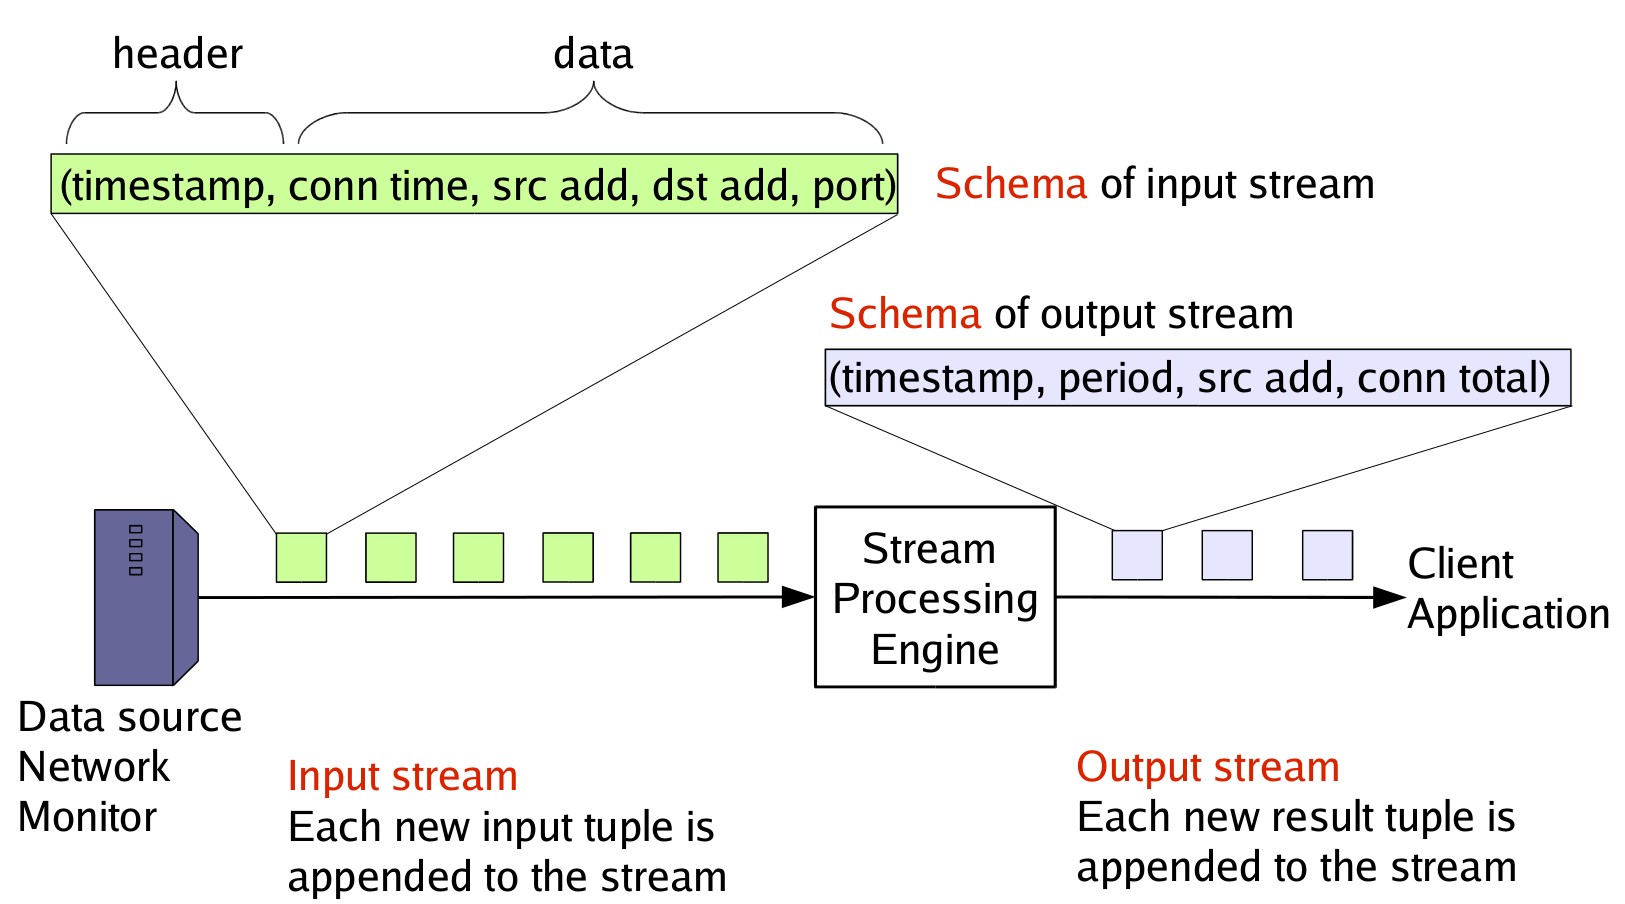
\includegraphics[width=0.8\textwidth]{images/streams_schemas.png}
	\caption[Data stream and schema]{Data stream and schema \cite{balazinska2005fault}}
	\label{fig:sps_data_stream}
\end{figure}

Data streams are produced by external entities (in relation to the SPS) called \emph{data sources}. The data produced by a data source is made available for consumption through a data pipeline, such as a socket, a file system or a more sophisticated message system. The produced data is ingested by the SPS for processing through a component called \emph{source} or \emph{edge adaptor}. This component receives the data in real-time and forwards it to the downstream operators.

An operator, according to Andrade, Gedik and Turaga \cite{andrade2014fundamentals}, is the basic functional unit of an application. An operator receives as input one or more data streams, applies some function to a single tuple or a set of tuples, and generates one or more output streams. Operators have \emph{input} and \emph{output} ports, which are logical communication interfaces that allows them to receive and emit tuples to data streams, with each one port being associated to a single data stream.

Some of the more common tasks performed by operators are:

\begin{itemize}
\item Parsing/Filtering/ETL;
\item Aggregation: collection and summarization of tuples;
\item Merging: combining of streams with different schemas;
\item Splitting: partitioning of stream into multiple ones for data/task parallelism of some logical reason;
\item Data mining/Machine Learning/Natural Language Processing: spam filtering, fraud detection, recommendation systems, clustering, sentiment analysis;
\item Others: relational algebra, artificial intelligence, computer vision, and other custom operations.
\end{itemize}

According to Gulisano et al \cite{gulisano2010streamcloud}, operators can be classified as stateless and stateful. Stateless operators only need the current tuple in order to produce any results (e.g. map, filter), while stateful operators need more than one tuple (e.g. join, aggregation). Stateful operators can be further classified as either blocking or non-blocking. A non-blocking operator is one which, although storing data about past tuples, can produce results after each new tuple processed.

A blocking operator, on the other hand, requires the whole dataset in order to produce a result, such is the case of a join or frequent itemset operator. But since a data stream is unbounded in size it is impossible for such operator to ever produce any results. To overcome this restriction tuples can be grouped in windows based on a range of time units or a number of tuples. Each window has a start ($W_s$), an end ($W_e$) and an advance parameter ($Advance$). Different configurations for these parameters may create windows of fixed or variable size, with or without overlap between windows \cite{gulisano2012streamcloud}.

Stream processing applications (SPAs) are also bound to other restrictions, such as the limited processing time and memory, as they need to produce results in a timely manner and to do so they must keep all data in memory, which is limited (and small if compared to the hard disk), and the amount of processing lean. For some applications these requirements were so important that they were willing to trade the accuracy of the results for a smaller latency (time between ingestion of a tuple and production of results).

These approximate operators are usually based on \emph{synopsis structures} \cite{aggarwal2007survey}. The main examples of synopsis structures and their practical use are:

\begin{itemize}
\item Sampling: classification, query estimation, order statistics estimation, distinct value queries;
\item Wavelets: hierarchical decomposition and summarization;
\item Clustering: knowledge discovery;
\item Sketches: distinct count, heavy hitters, quantiles, change detection;
\item Histograms: range queries, selectivity estimation.
\end{itemize}

On the other end of an application is the \emph{data sink}, which is similar to a normal operator, except for the fact that it does not produce any output streams. A data sink has the purpose of exporting the results of a SPA, either to a database or to another system, for visualization or further processing.


% Programming Model
In stream processing an application is usually composed as a flow graph with nodes as operators and directed edges as data streams and the communication follows the publish-subscribe model. There are, however, different programming models for stream processing:

\begin{itemize}
\item DAG (Directed Acyclic Graph): a directed graph without cycles.
\item Actors model: an actor is a computational entity that can respond to a message by sending messages to other actors, creating new actors and designating the behaviour for the next message it receives, all in parallel.
\item Monad: originated from functional programming, it is a structure that represents a chain of operations.
\end{itemize}

% Parallelism
The parallelism of SPAs (Figure \ref{fig:sps_parallelism}) can be expressed in three ways: \emph{pipeline}, \emph{data} or \emph{task parallelism}. The \emph{pipeline parallelism} works similarly to the way a CPU processes instructions, with instructions being analogous to operators. In order for task parallelism to work properly an application must have the right level of decomposition, in order to accomplish a good usage of computational resources.

\emph{Data parallelism} consists on the execution of the same task over different data items or Single Instruction Multiple Data (SIMD). This type of parallelism depends on the nature of the operator: \emph{stateless}, \emph{partitioned-stateful} or \emph{stateful}. Obviously, the simpler case lies in the \emph{stateless} operators, because the workload can be evenly distributed among their instances without any worries about dependencies between tuples. With \emph{partitioned-stateful} operators, however, some sort of consistency must be followed when splitting a data stream among an operator's instances. With \emph{stateful} operators simply choosing a partitioning configuration is not enough, it usually involves operators dedicated specifically for splitting, merging and re-ordering the tuples.

The most common partitioning configurations are:

\begin{itemize}
\item Shuffling: tuples are randomly and evenly distributed.
\item Group By: tuples are distributed accordingly to the value of one or more fields.
\item Broadcast: the entire data stream is replicated to all subscribers.
\item Directed: tuples are distributed directly to a selected subscriber.
\end{itemize}

\begin{figure}[!ht]
	\centering
	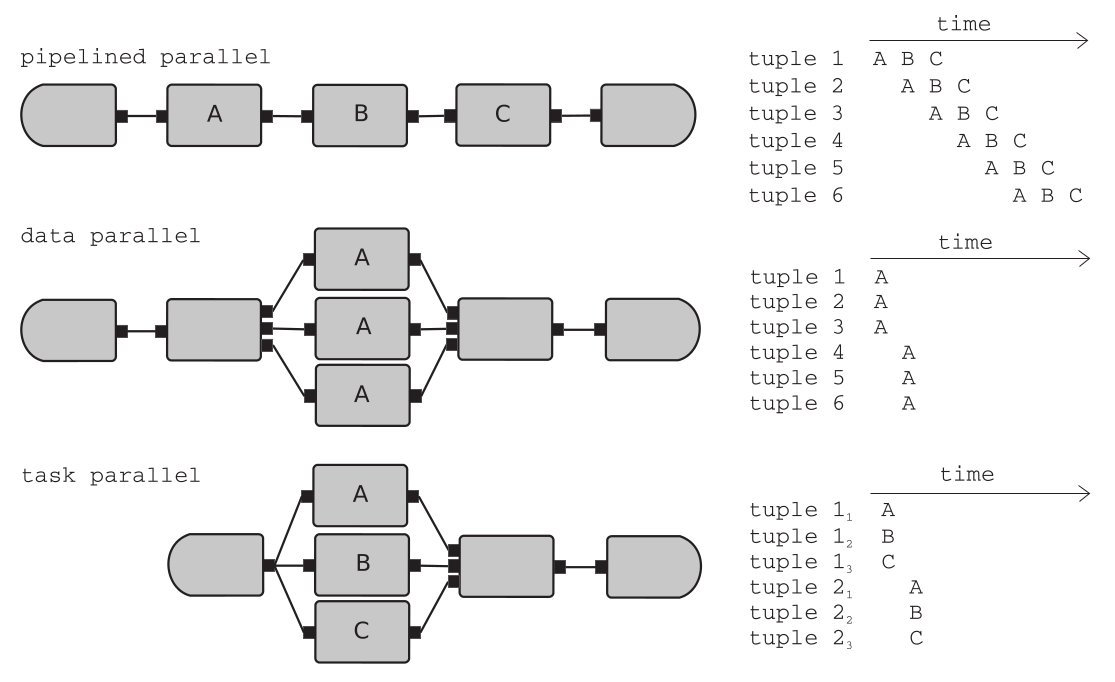
\includegraphics[width=0.8\textwidth]{images/sps_parallelism.png}
	\caption[Types of parallelism in stream processing]{Types of parallelism in stream processing \cite{andrade2014fundamentals}}
	\label{fig:sps_parallelism}
\end{figure}

At last, the \emph{task parallelism} is closely related to the nature of SPAs, as they are a composition of tasks that, in many cases, work in parallel. But even if the task parallelism is almost unavoidable in an SPA, it is paramount to ensure the balance between these tasks in order to improve the performance and avoid waste of resources, such as extra memory usage due to large queues of tuples waiting to be merged.


% processing models
Another important aspect of SPSs is the way the processing of tuples is carried out. The first approach used is the \emph{record-at-a-time}, which means that each tuple is processed by the operators individually, providing a very low latency. There are however two main downsides of this approach: lower throughput and high overhead for tracking message delivery. To overcome these shortcomings some SPSs process data streams in \emph{mini-batches} \cite{muralidharan2014fault}, which tends to increase the throughput, at the cost of an increase in latency. It also means that the system needs only to track the delivery of the batches instead of individual tuples.


\section{History}
\label{sec:esp:history}

Stream Processing is only one among a series of systems developed for processing large volumes of data in real-time and giving information to act upon in a timely manner, all of them part of what is called \emph{Information Flow Processing} (IFP). The early IFP systems helped pave the way to the modern SPSs in the market which, according to Andrade, Gedik and Turaga \cite{andrade2014fundamentals}, are: 

%\emph{active databases}, \emph{Continuous Query} (CQ) systems, \emph{publish-subscribe} systems and \emph{Complex Event Processing} (CEP) systems \cite{andrade2014fundamentals}.

\begin{itemize}
\item \textbf{Active databases} rely on ECA (Event-Condition-Action) rules in order to capture events, the surrounding conditions and the actions to be taken in case the conditions are met. Current DBMSs implement these active database features with \emph{triggers} defined using SQL.

\item \textbf{Continuous Queries} are known as \emph{standing} queries as opposed to relational database queries (\emph{snapshot} queries), because they continuously monitor incoming information, producing a stream of results. A CQ is composed of a \emph{query}, a \emph{trigger} which will activate the query, and a \emph{stop condition} which will determine when the query should stop to compute updates.

\item \textbf{Publish-subscribe} system is composed of \emph{publishers} that produce data and \emph{subscribers} that consume that data in the form of messages. The components of a pub-sub system have no knowledge of each other, and the delivery of message lies upon a \emph{broker network} composed of brokers nodes. There are two categories of pub-sub systems defined accordingly to how consumers subscribe to data.

In a \emph{topic-based} pub-sub system, consumers simply subscribe to topics and receive all data produced by publishers in those topics, a characteristic that simplifies the routing of messages within the broker network. With a \emph{content-based} pub-sub system however, the routing is much more complex, because each message must be evaluated in order to determine to which subscribers it is going to be delivered. Each publication has a set of properties and each subscription defines a set of conditions based on these properties.

\item \textbf{Complex Event Processing} systems collect, filter, aggregate, combine and correlate events originated from multiple sources in order to create more complex events and/or take action based on the detected events \cite{robins2010complex}.
\end{itemize}


% three generations - must quote Heinze (2014)

According to Heinze et al \cite{heinze2014cloud}, the history of SPSs can be broken in three generations:

In the \emph{first generation}, systems were devised to work in a single node (centralized) with applications developed using query languages derived from SQL, but continuous instead of snapshot-based, or visual languages (boxes and arrows). The use of SQL as foundation happened in some cases because these systems were using relational database engines underneath.

Among the first SPSs developed the most notable are the TelegraphCQ, developed at the University of California, Berkeley; STREAM, developed at Stanford University; and Aurora, developed by a collaboration between the Brandeis University, Brown University and MIT.

The \emph{second generation} went a step further, with systems working on very large networks, mainly for processing data from sensor networks, which means that the processing must occur in a distributed fashion.

In this period a lot of research was built on all aspects surrounding SPSs, such as job and resource management, scheduling, load balancing, high availability, monitoring, fault tolerance, QoS, visualization, stream algorithms and query languages. In comparison with the the first generation, now the systems have a much wider range of operators, as well as the ability to build custom operators. Examples from this generation are: Borealis, CEDR, System S and CAPE.

In the \emph{third generation} there is a shift towards massively-parallel systems, working on clusters instead of very large networks. These systems also favor general purpose languages instead of DSLs (Domain Specific Languages), giving the developer a wide range of possibilities for building applications. The focus is now on processing large volumes of data as fast as possible using clusters of computing nodes, usually with Cloud Computing. Examples from the third generation are: S4, Storm, Spark Streaming, Flink Streaming, Samza and Apex.

\begin{figure}[!ht]
	\centering
	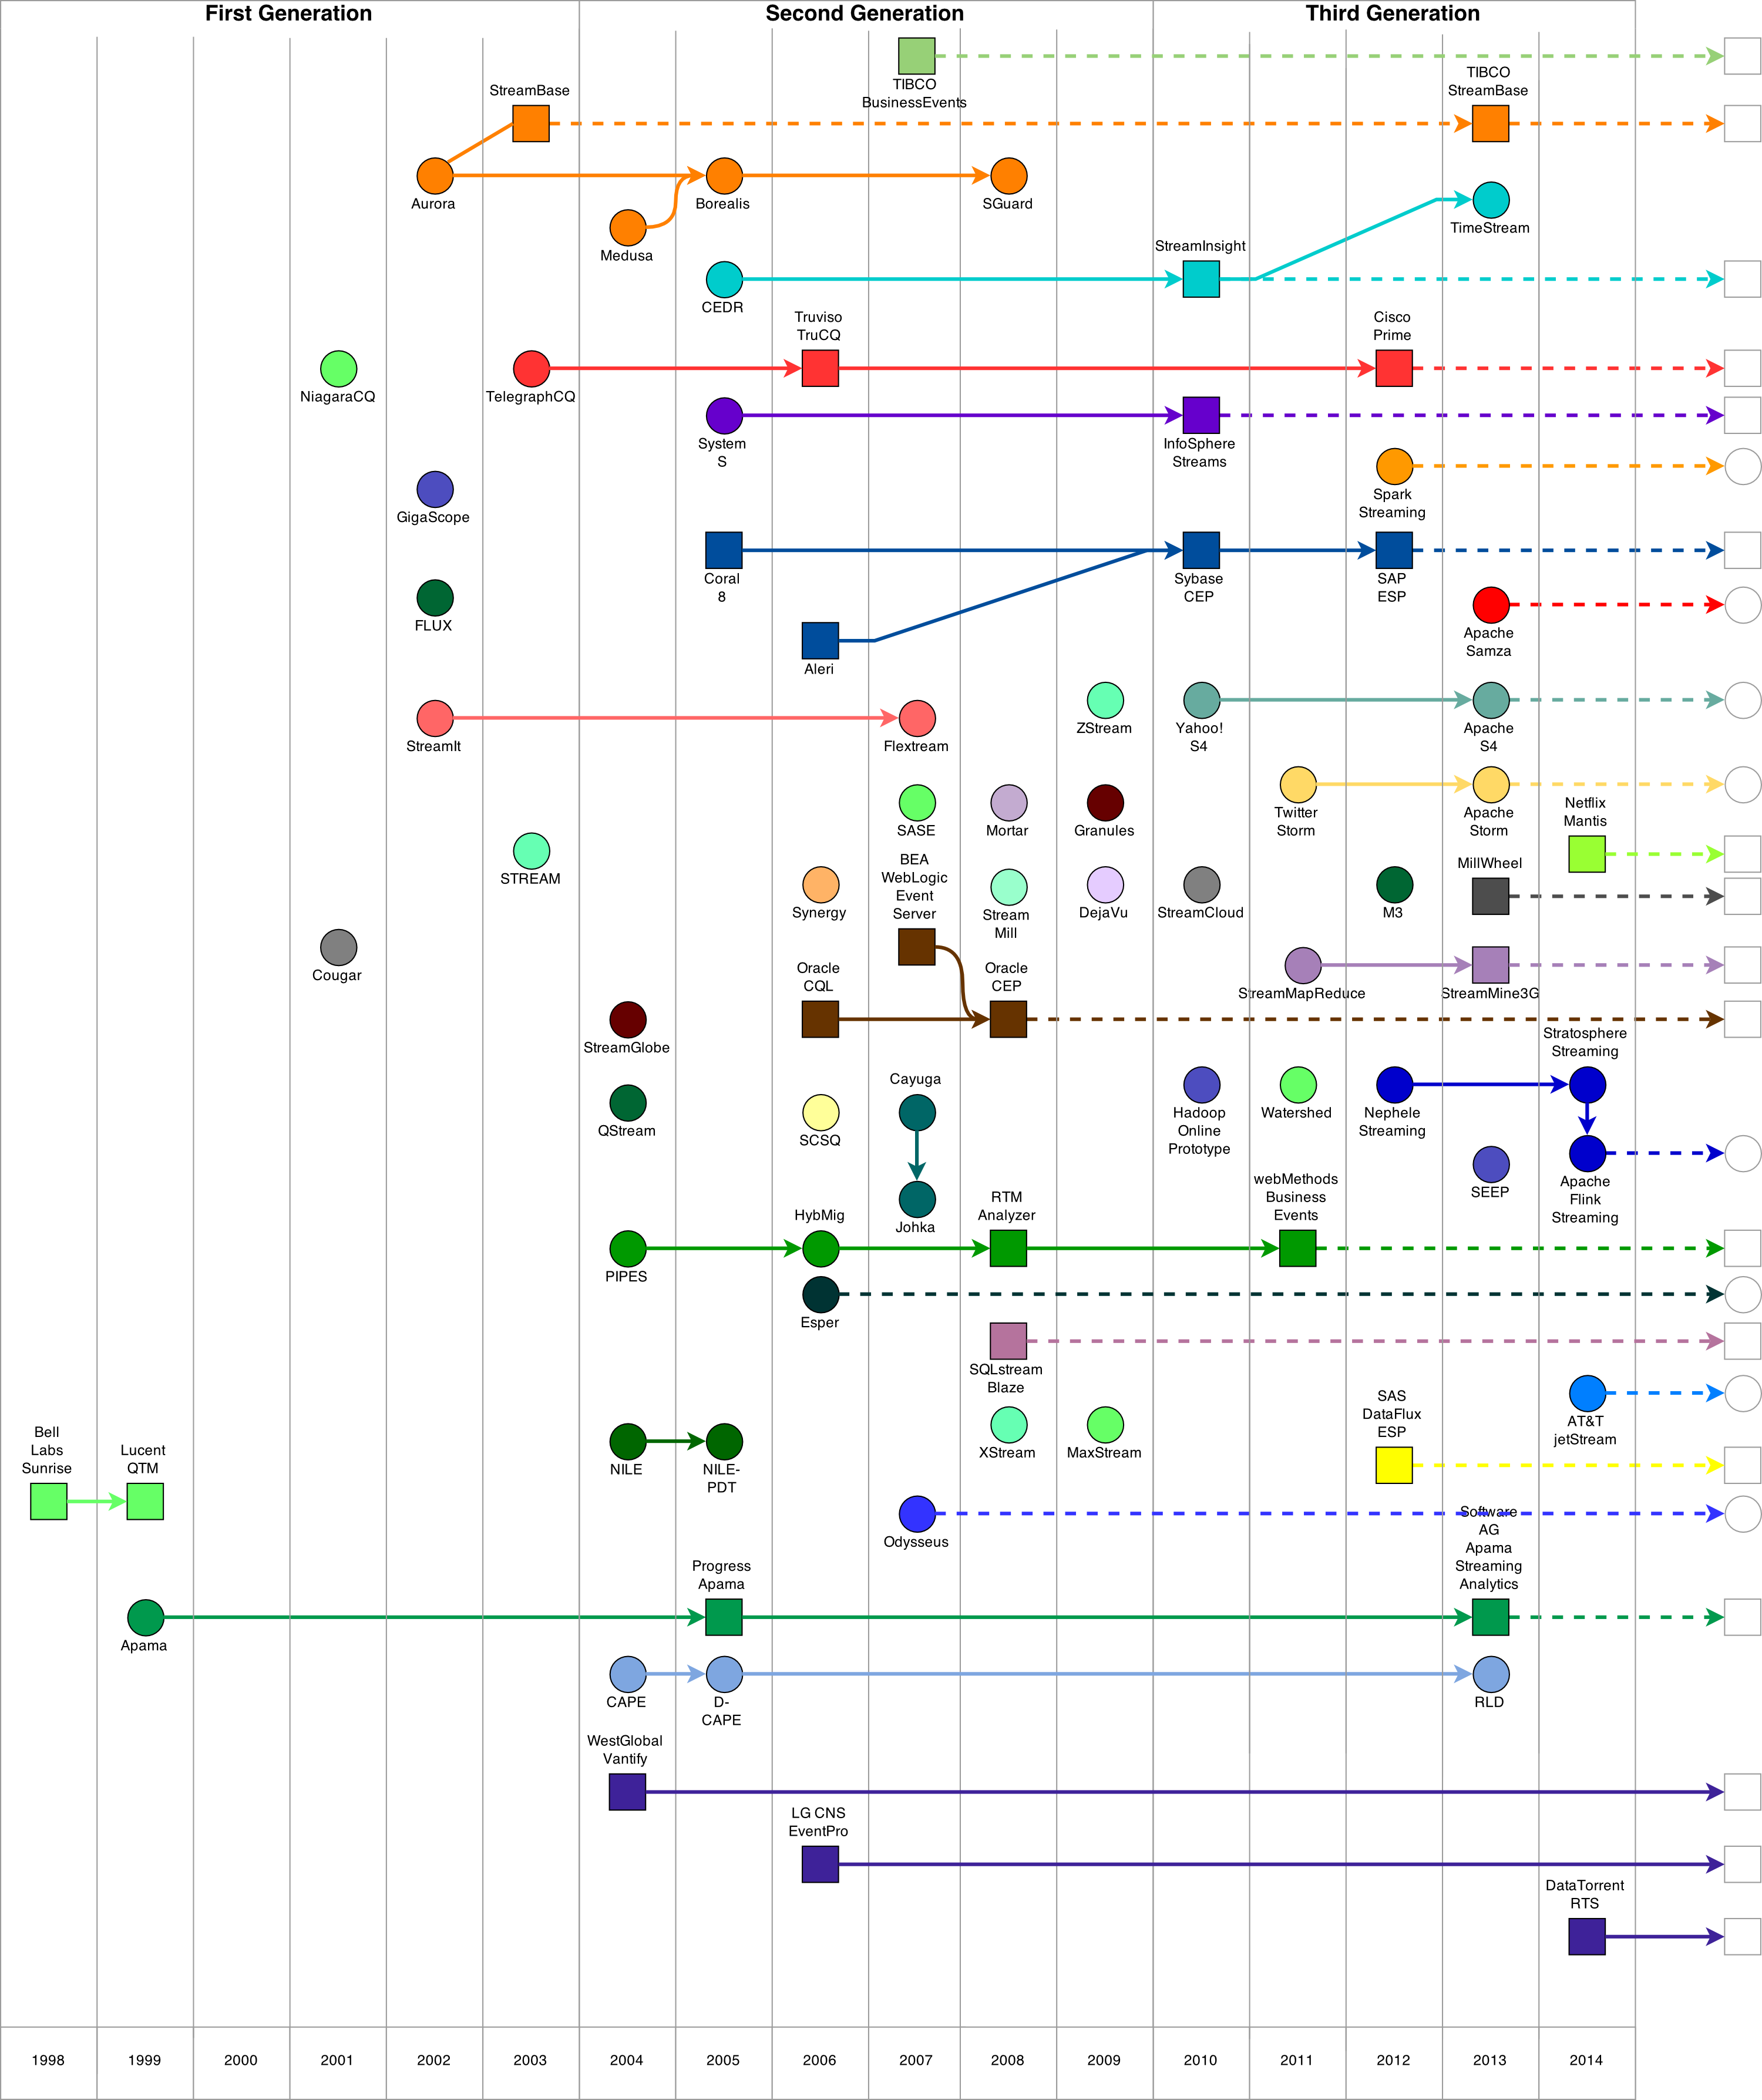
\includegraphics[width=0.8\textwidth]{images/history.pdf}
	\caption[Timeline of SPSs]{Timeline of SPSs \cite{heinze2014cloud}\cite{paulvincent2014}}
	\label{fig:sps_history}
\end{figure}


\section{Operator Placement and Load Balancing}
\label{sec:esp:scheduling_load_balancing}

Meeting QoS requirements is not an easy task as it usually involves balancing aspects that most of the time work against each other. In a environment where data can present bursts of volume, a system has to be able to cope with it, while maintaining the established QoS.

In an SPS, the operators of a query will be spread across multiple computing nodes, thus meeting the QoS requirements means finding a good operator placement and since stream loads can greatly vary along time, these systems should also employ good load balancing techniques.

%%

The processing graph is considered the logical representation of the query which will be used by the scheduler in the placement of operators. The mapping of operators to computing nodes will create the physical representation of the query, where the vertices now represent the nodes \cite{kossmann2000state, lei2012robust}.

One of the main differences in the way the scheduler works depends on the type of \textbf{load partitioning} supported by the system \cite{johnson2008query}. \textbf{Data stream partitioning} allows an operator to be placed in several nodes, distributing the load among them. Whereas in \textbf{query plan partitioning} one operator can live only in one node, with the disadvantage that if an operator consumes more resources then a machine can offer, the only solution is to upgrade the machine or apply some technique of admission control.

Following the taxonomy defined by Casavant and Kuhl \cite{casavant1988taxonomy} another important aspect of schedulers for DSPSs is the time at which the operator placement is made (\textbf{statically} or \textbf{dynamically}). Giving the variable nature of data streams most schedulers proposed in the literature approach the problem with a initial operator placement and an online load balancing, with special attention to the management of bursts.

More recently a taxonomy was proposed \cite{lakshmanan2008placement} specifically for SPSs. The authors propose six core components that describe placement algorithms:

\begin{itemize}
    \item \textbf{Architecture}: whether is an \emph{independent module} from the system, a \emph{distributed} one with each node executing an instance of it, or an \emph{hybrid} of both approaches.
    \item \textbf{Algorithm Structure}: if the algorithm has knowledge of the entire network's state it is \emph{centralized}, otherwise it is \emph{decentralized}, using only local knowledge to make decisions.
    \item \textbf{Metrics}: used in the objective functions in order to optimize the placement of operators. Commonly used metrics are the \emph{load}, \emph{latency}, \emph{bandwidth}, \emph{machine resources} and \emph{operator importance}.
    \item \textbf{Operator-Level Operations}: describes the operations supported by the operators in order to improve the performance of the operator placement algorithm, such as reusing an operator that appears in more than one query (\emph{operator reuse}) and replicating one operator to improve the performance (\emph{replication}).
    \item \textbf{Reconfiguration}: ability of the algorithm to adapt in order to cope with changes in the network, input rate or application components.
    \item \textbf{Response Strategies}: some algorithms requires the application to stop in order for a new placement to be calculated, while other algorithms can dynamically respond to changes by migrating operators or redistributing the load among the operators or, if possible, using some technique such as \emph{load shedding}.
    \item \textbf{Change Triggers}: operator migration can be triggered if certain performance threshold has been trespassed, a constraint has been violated, or by periodically checking if the gain from migrating an operator is greater that the cost of moving it.
\end{itemize}

\section{Fault Tolerance}
\label{sec:esp:fault_tolerance}

Fault tolerance in SPSs is of utmost importance due to the fact that its applications have to run for large periods of time. An SPS can suffer from node crashes and partitions, component and networks failures.

It has to guarantee that the state of the system is consistent and that all messages received are processed. In order to accomplish that some techniques can be employed. In the next paragraphs the main techniques, according to Gradvohl et al \cite{gradvohl2014comparing}, will be described.

\textbf{Replication of components}, as the name suggests consists of replicating a component of the system so that in case of a failure the replicated component can take over the failed one. The replication can happen \emph{actively}, meaning that the replicated component receives the same input as the main component, and in case of a failure the replicated component can take over immediately. The drawback is that the cost of the component is also duplicated. The other approach is the \emph{passive} replication, and in this case the replicated component is dormant, and in case of a failure all the input processed by the failed component has to be replayed to the replicated component. Depending on the size of the input to be replayed the time required for the component to reach the same state as the failed component can be intolerable. To overcome this, the technique that will be described next can be used.

\begin{figure}[!ht]
	\centering
	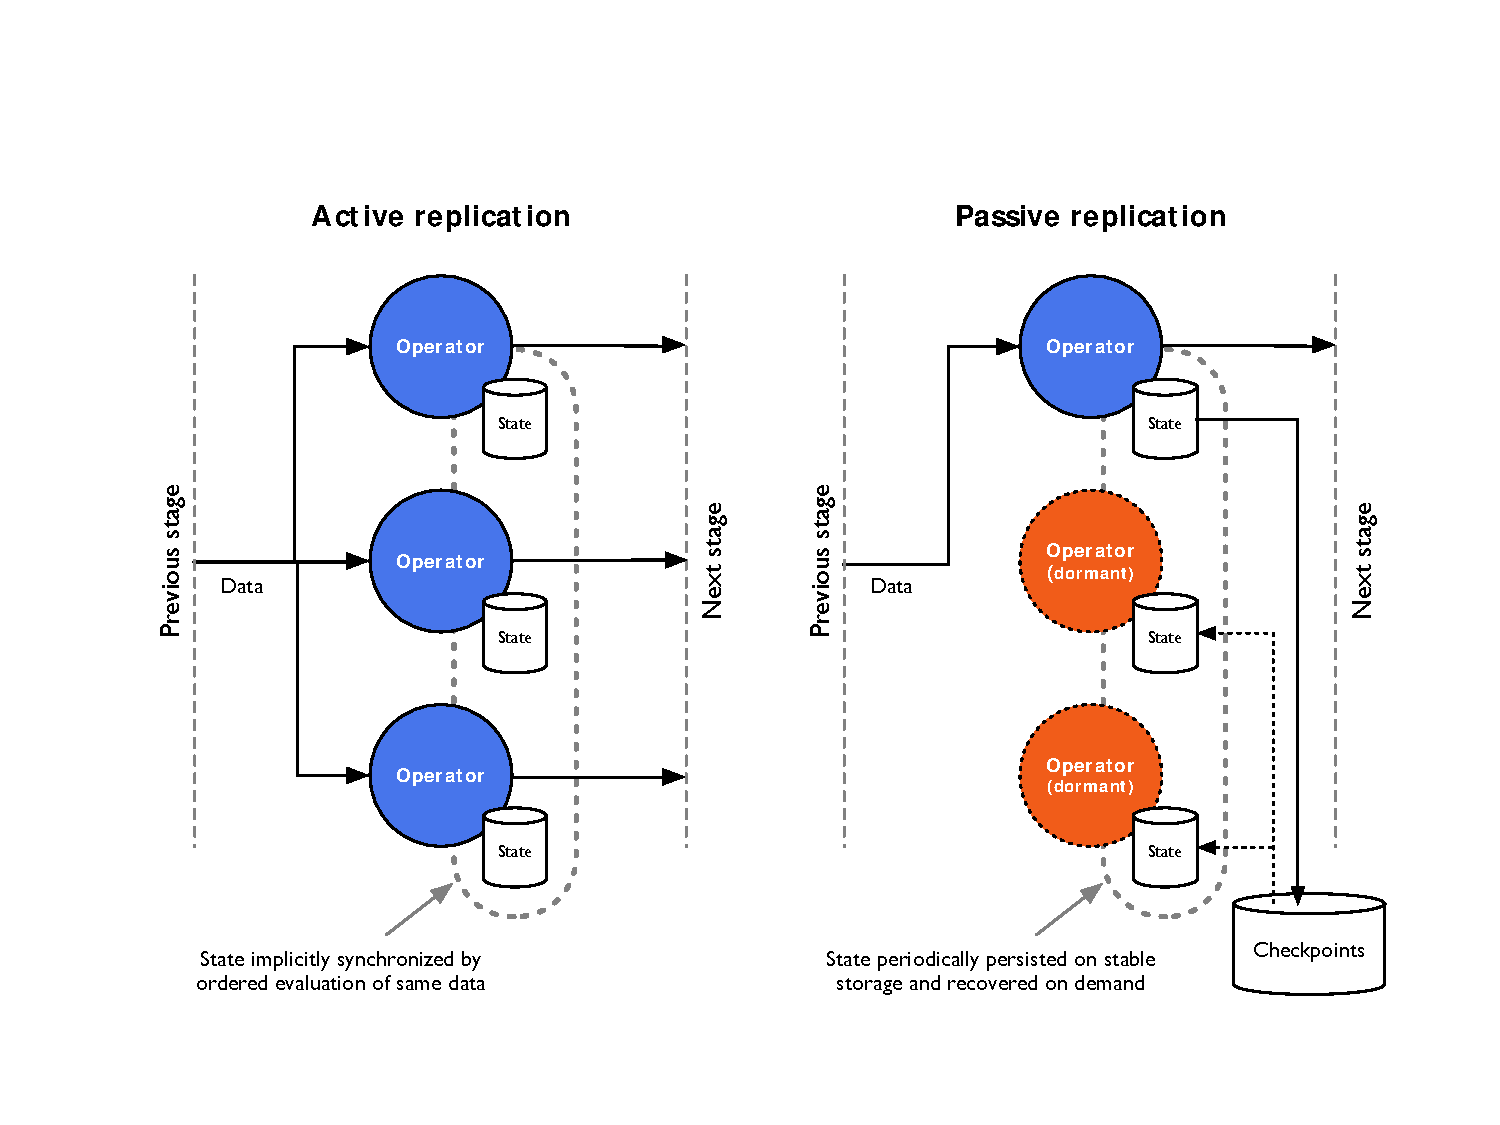
\includegraphics[width=0.8\textwidth]{images/fault_tolerance/replication.pdf}
	\caption[Replication of components]{Replication of components \cite{heinze2014cloud}}
	\label{fig:ft_replication}
\end{figure}

\textbf{Checkpointing} consists of saving the state of the system periodically to a stable storage, enabling the recovery of the state in case of a failure. Checkpoints can be \emph{uncoordinated}, with each process deciding when to make the checkpoint, which can lead to system inconsistencies; or \emph{coordinated}, where all processes agree on when to checkpoint, thus requiring the exchange of messages between them.

\begin{figure}[!ht]
	\centering
	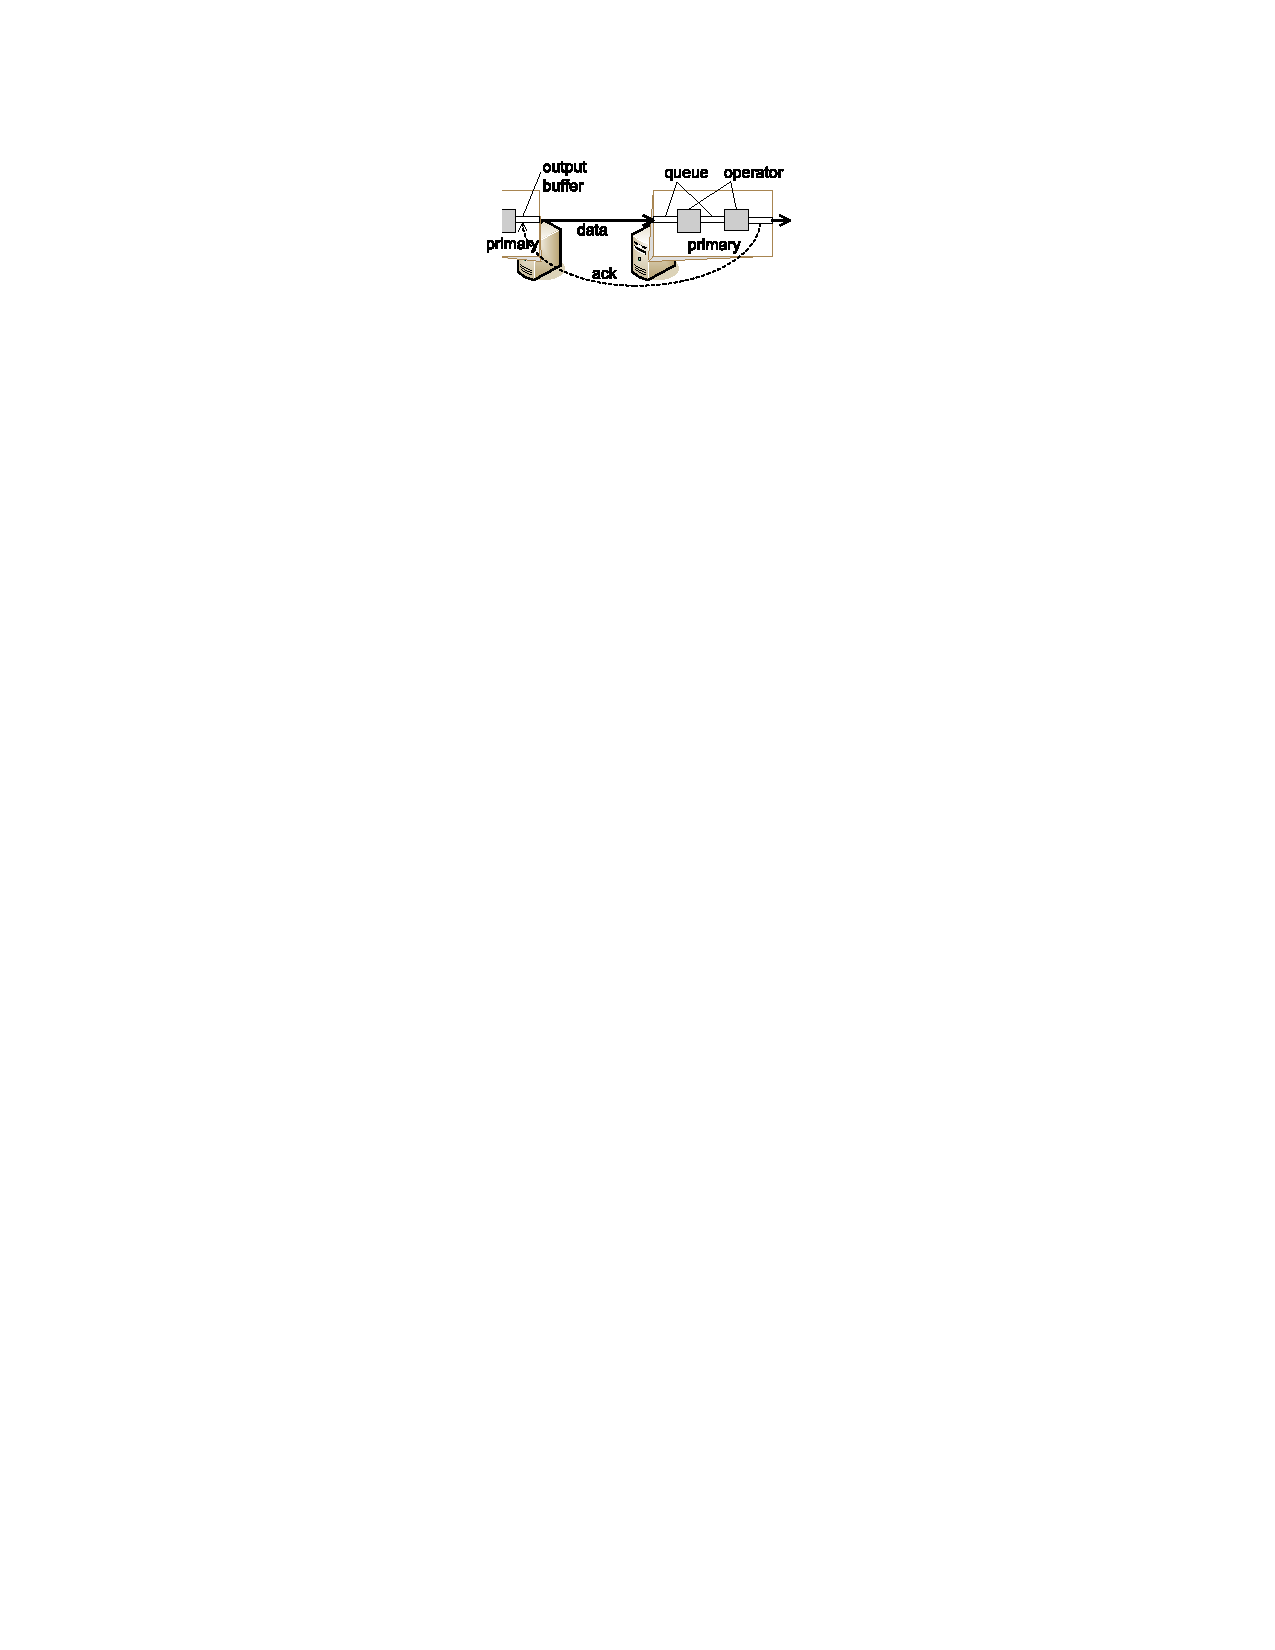
\includegraphics[width=0.6\textwidth]{images/fault_tolerance/upstream_backup.pdf}
	\caption[Upstream backup]{Upstream backup \cite{balazinska2009fault}}
	\label{fig:upstream_backup}
\end{figure}


\textbf{Upstream backup} requires a node to save the tuples it is sending to downstream nodes in a queue until the downstream nodes have processed them (\emph{ack} messages). In case of a failure the node can send the tuples again. It can become a problem if the size of the queue grows outside the main memory.

\textbf{Recovery} is classified as \emph{precise}, when all tuples not processed by the downstream nodes are sent, the failure is completely masked (except for the delay in processing); on \emph{roll-back} recovery the output may be different from that of a failure-free execution as some tuple may be duplicated; and in \emph{gap} recovery some tuples may be lost in order to reduce the recovery time.


\section{Message Systems}
\label{sec:esp:data_transport}

According to Bockermann \cite{bockermann2014survey} a \emph{queueing} or \emph{message passing} component is one of the two main functionalities of an SPS, the other being the \emph{execution engine} itself. The message system will be responsible for connecting the components of an SPS, transporting tuples from producers to consumers, ensuring that the connections are fault-tolerant and are performing well regarding throughput and latency \cite{andrade2014fundamentals}.

Systems such as S4 used to rely solely on TCP, changing later to the Netty library. Storm did something similar, changing from ZeroMQ to Netty. And while these systems rely on libraries to handle their communication, some systems prefer to use a middleware, as is the case of Apache Samza which uses Kafka as its message system. Other examples of middlewares are RabbitMQ and ActiveMQ.

% Kafka, middlewares (netty), etc.

\section{Platforms}
\label{sec:esp:platforms}

In this section the most prominent SPSs in the open source market are described. It is assumed that the basic concepts of stream processing are known (Section \ref{sec:esp:concepts}). The descriptions focuses mainly o programming and architectural characteristics. At the last section there is a qualitative comparison of the platforms, highlighting their similarities and differences.

\subsection{Storm}

Storm is an open source distributed real-time computation system. Applications are called \emph{topologies} and they are built as DAGs, with \emph{spouts} as data sources and \emph{bolts} as operators, the communication between these components happens through \emph{streams}. Each component can declare the streams, and their respective schemas, that he is going to produce, however, only bolts can subscribe to streams.

The data parallelism is provided by Storm through what is called \emph{stream grouping}. By default there are seven options:

\begin{enumerate}
\item \textbf{Shuffle grouping}: tuples are random and evenly distributed among bolt's tasks.
\item \textbf{Fields grouping}: tuples are grouped by the specified fields, meaning that tuples with the same value for the grouping field will always go to the same task.
\item \textbf{All grouping}: all tasks receive all the tuples, i.e. the stream is replicated.
\item \textbf{Global grouping}: the entire stream goes to the task with the lowest ID.
\item \textbf{None grouping}: currently it is the same as the \emph{shuffle}, but eventually it will try to put the subscriber task in the same thread as the publisher.
\item \textbf{Direct grouping}: the publisher of the tuples chooses the task to which the tuple will be sent.
\item \textbf{Local or shuffle grouping}: if the subscriber has one or more tasks in the same worker process as the publisher, the tuples will be shuffled only among them, otherwise it will act just like a normal shuffle.
\end{enumerate}

The parallelism of each component is defined at declaration, as seen in Figure \ref{fig:storm_topology_parallelism}. In Storm this is the number of \emph{executors} or threads that will be spawned for each component by a \emph{worker}, which is a process that resides in one machine of a Storm cluster and runs executors of one topology. Executors run one or more \emph{tasks}, which are the ones that perform the data processing.

\begin{figure}[!ht]
	\centering
	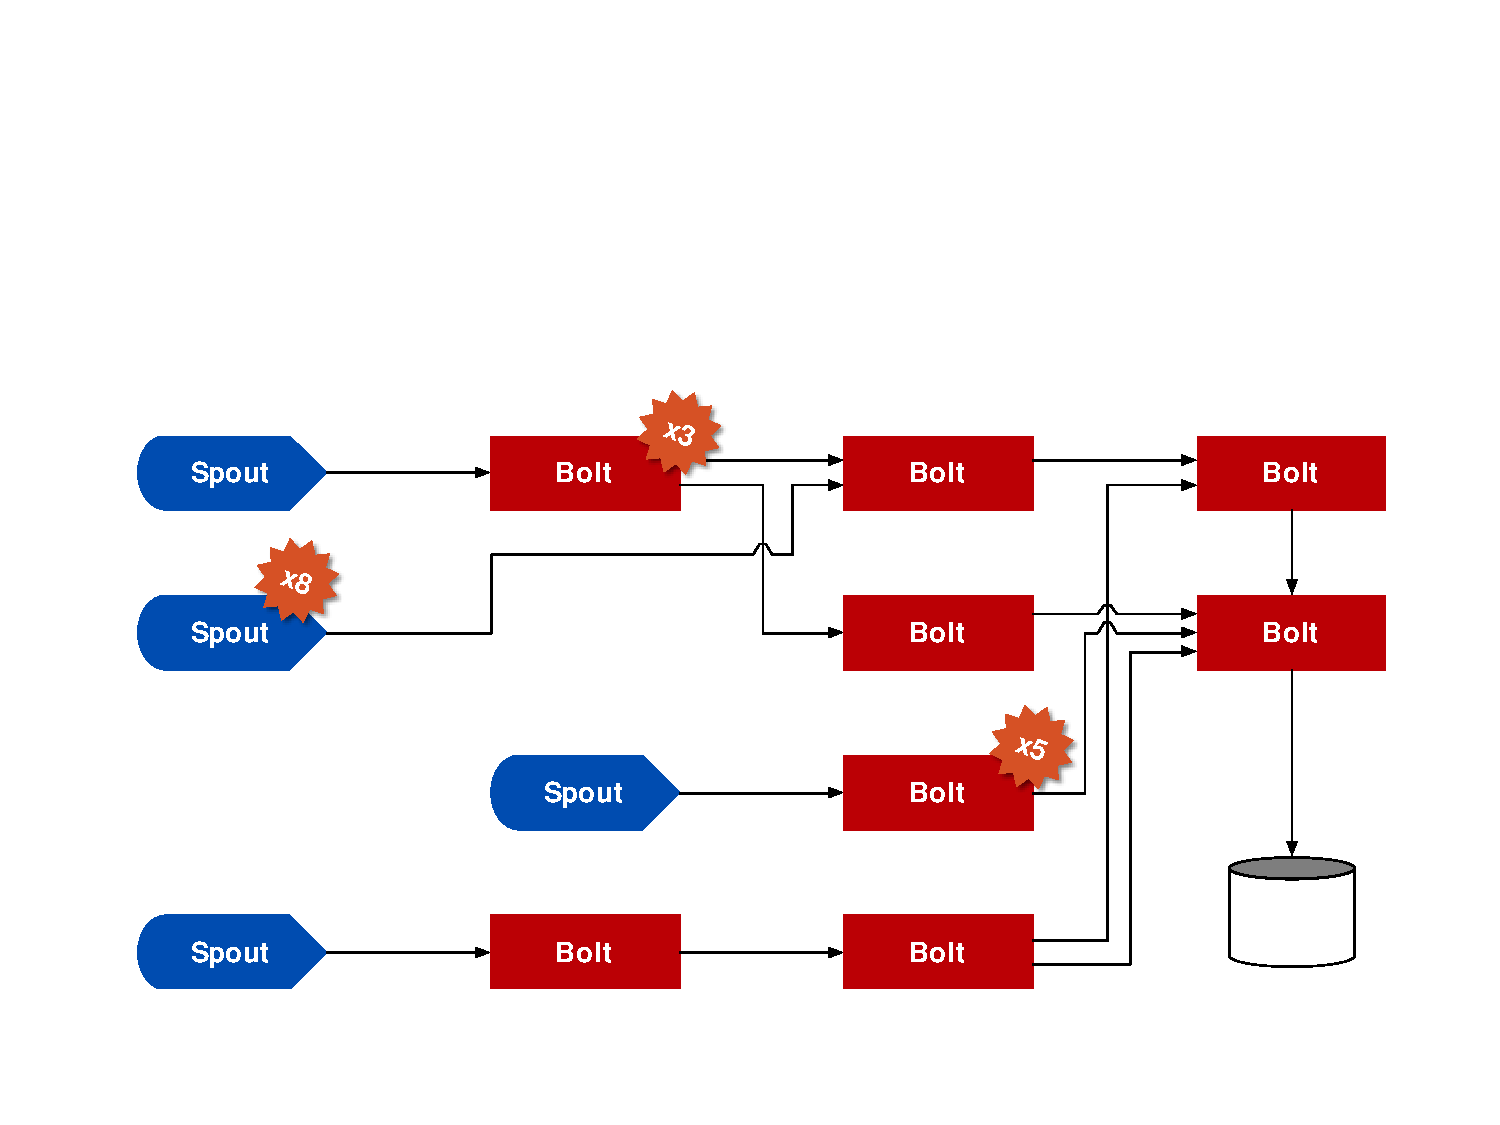
\includegraphics[width=0.6\textwidth]{images/storm/topology_parallelism.pdf}
	\caption[Storm topology components and parallelism]{Storm topology components and parallelism \cite{heinze2014cloud}}
	\label{fig:storm_topology_parallelism}
\end{figure}

In Figure \ref{fig:storm_running_topology} it is possible to see an example of a running topology with two workers, one spout configured with two executors and two tasks, a green bolt with two executors and four tasks, and a yellow bolt with six executors and six tasks.

\begin{figure}[!ht]
	\centering
	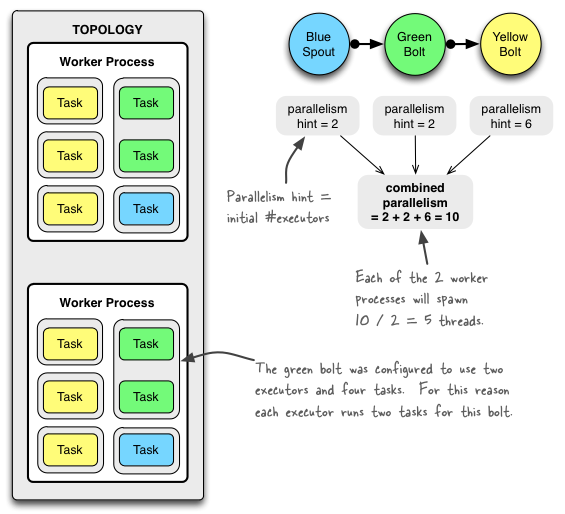
\includegraphics[width=0.6\textwidth]{images/storm/example-of-a-running-topology.png}
	\caption[Example of a running topology in Storm]{Example of a running topology in Storm \cite{storm2015docs}}
	\label{fig:storm_running_topology}
\end{figure}

A Storm cluster (Figure \ref{fig:storm_cluster}) is composed of one \emph{Nimbus} (the master) and a set of \emph{supervisors} (the workers). The Nimbus is responsible for assigning work to supervisors, as well as starting and stopping workers accordingly; managing failures; and monitoring resource usages \cite{heinze2014cloud}. Supervisors have a parameter called \emph{slots}, which is the maximum number of workers that they can execute \cite{aniello2013adaptive}. The coordination between the Nimbus and the supervisors relies on a Zookeeper cluster. Moreover, all state of the nodes is kept on Zookeeper in order to avoid data loss in case of a failure, enabling nodes to restart after a failure and continue from where they left off \cite{storm2015docs}.

\begin{figure}[!ht]
	\centering
	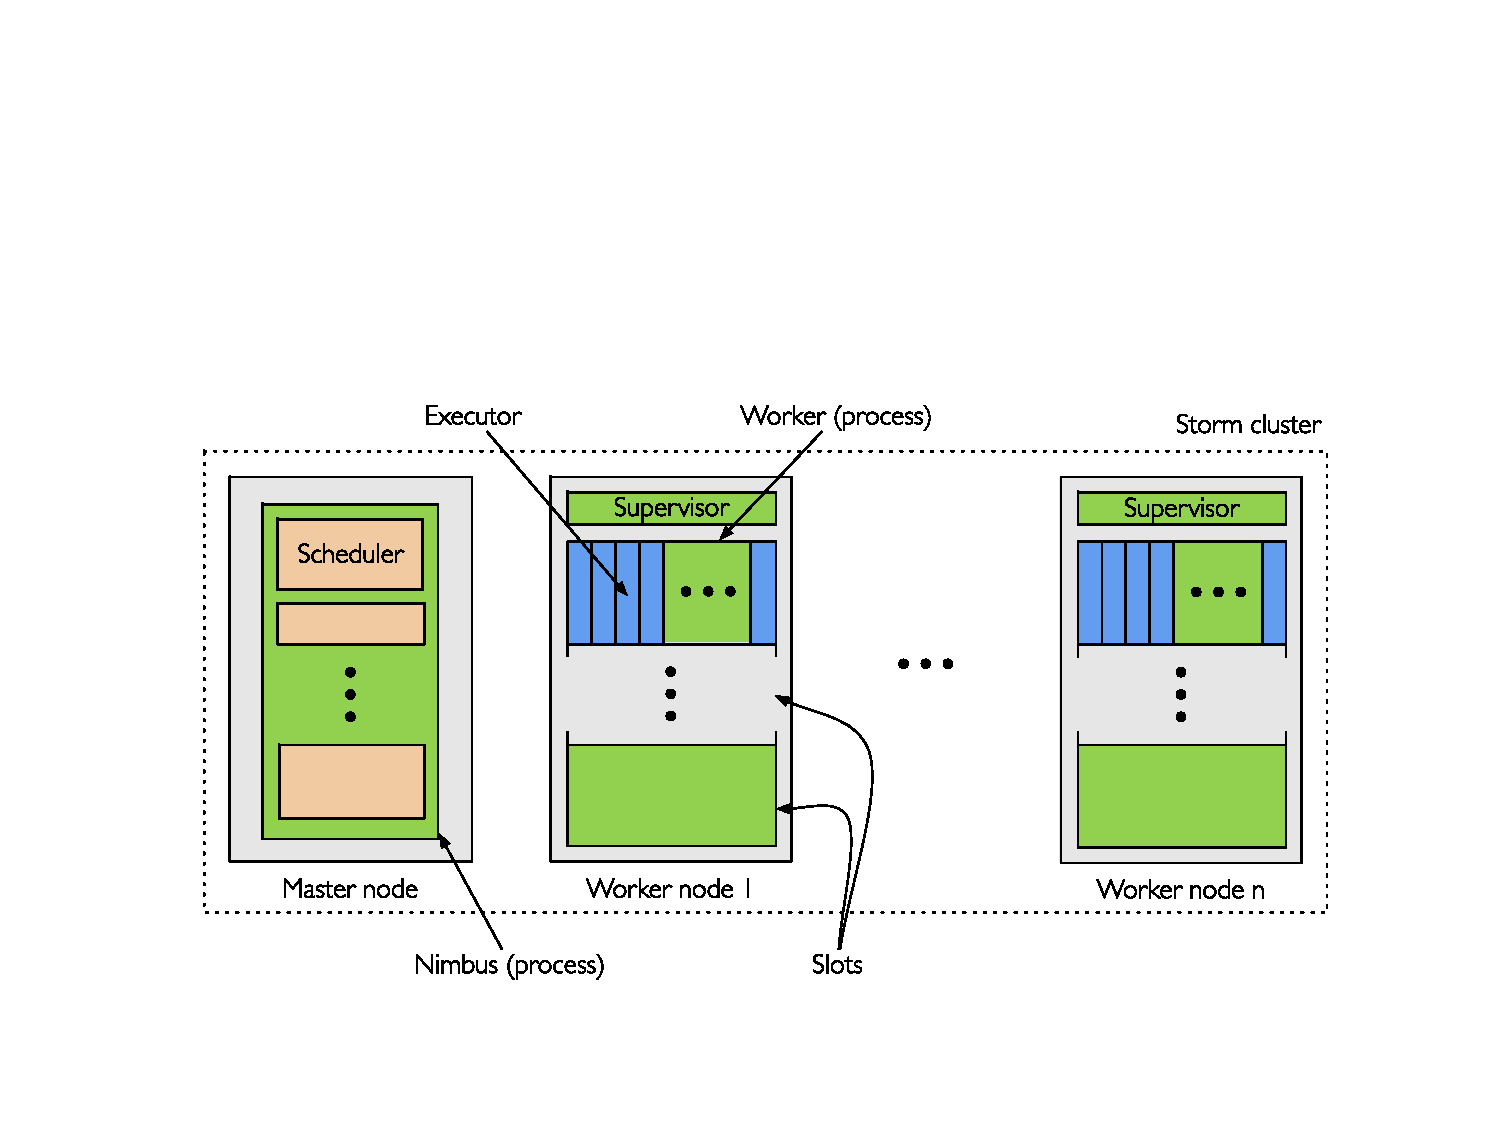
\includegraphics[width=0.8\textwidth]{images/storm/cluster.pdf}
	\caption[Storm cluster components]{Storm cluster components \cite{heinze2014cloud}}
	\label{fig:storm_cluster}
\end{figure}

When the Nimbus receives a topology it has to use a scheduler in order to assign executors to workers and workers to slots \cite{aniello2013adaptive}. The default scheduler of Storm (\emph{EvenScheduler}, Figure \ref{fig:storm_default_scheduler}) employs a round robin strategy for the assignment of executors to workers.

\begin{figure}[!ht]
	\centering
	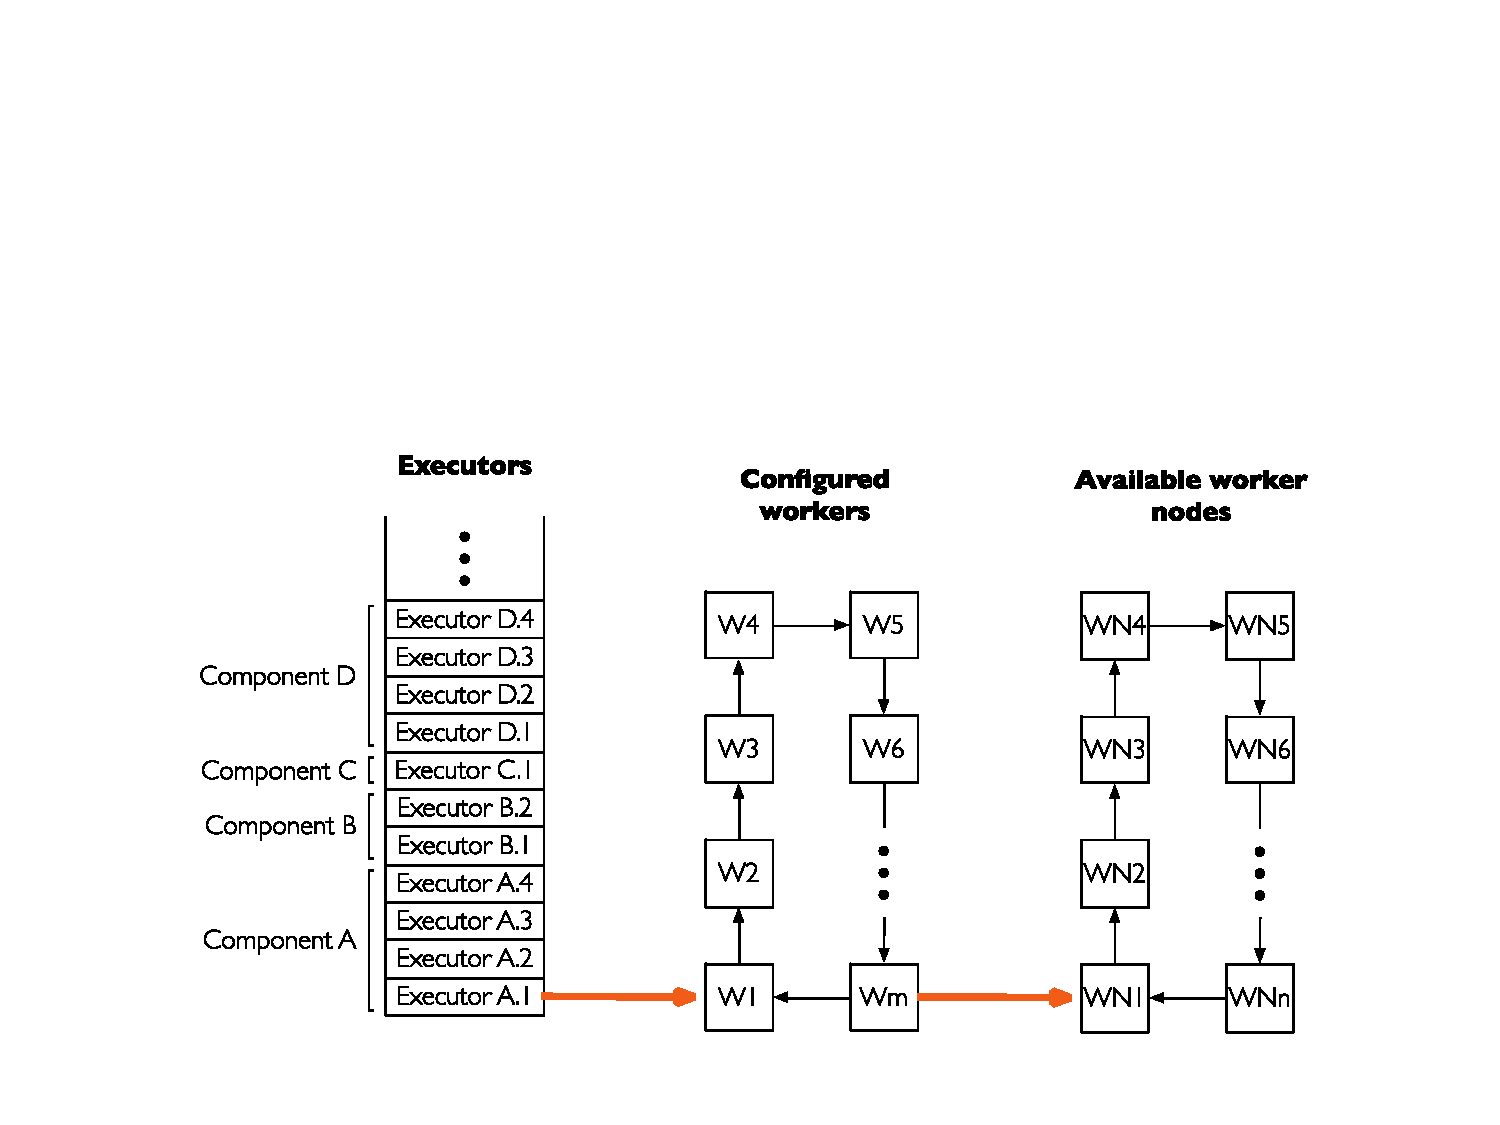
\includegraphics[width=0.6\textwidth]{images/storm/default_scheduler.pdf}
	\caption[Storm default scheduler]{Storm default scheduler \cite{heinze2014cloud}}
	\label{fig:storm_default_scheduler}
\end{figure}

Storm guarantees that all messages emitted by the spouts will be fully processed by keeping them on a queue until the confirmation that they have been processed, and in case a message has failed the spout will send it again \cite{gradvohl2014comparing}. To understand what "fully processed" means in Storm a simple example can be seen in Figure \ref{fig:storm_event_tracking}, it shows the \emph{tuple tree} which is composed of the original tuple and all tuples originated from that first tuple. After a tuple is processed in a bolt it is \emph{ack}'ed, after all tuples in the tuple tree have been ack'ed the message is considered fully processed.

\begin{figure}[!ht]
	\centering
	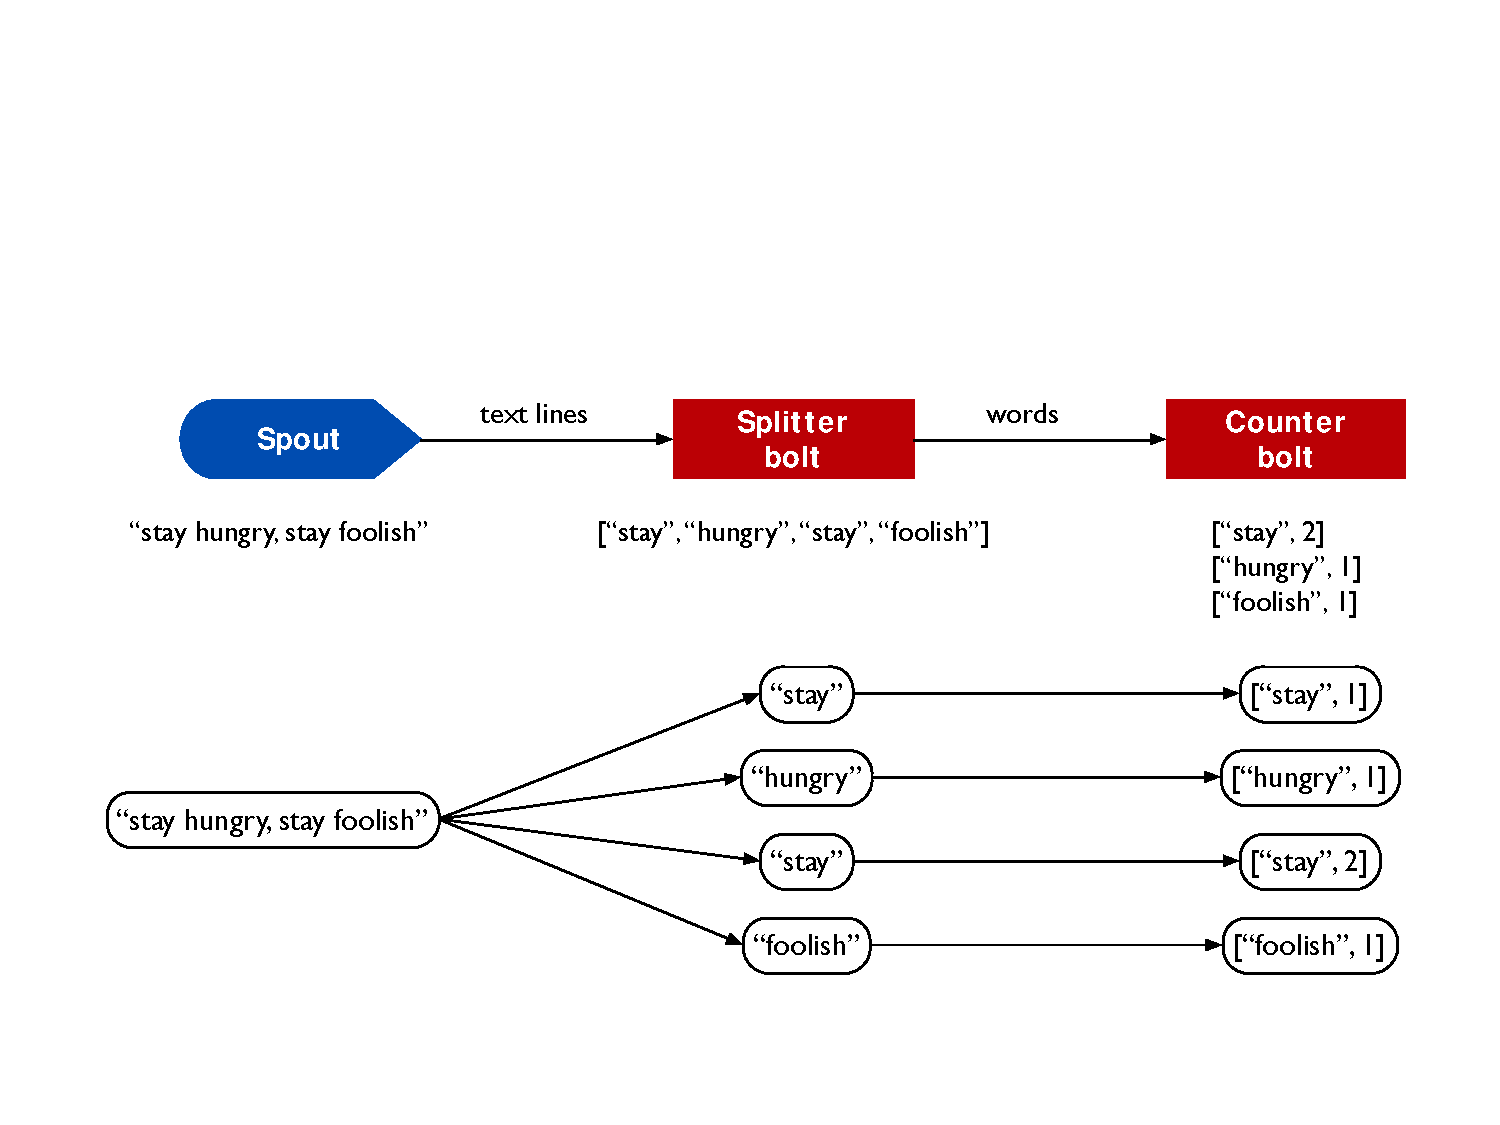
\includegraphics[width=0.6\textwidth]{images/storm/event_tracking.pdf}
	\caption[Storm event tracking]{Storm event tracking \cite{heinze2014cloud}}
	\label{fig:storm_event_tracking}
\end{figure}

\subsection{S4}

S4 is a framework for distributed stream processing based on the Actors model. Applications are built as a graph composed of \emph{processing elements} (PEs) that process events and \emph{streams} that interconnect the PEs. Events are made of a key and a set of attributes, and they are forwarded to a PE based on the value of the key, with exception of \emph{keyless} PEs.

In fact, the parallelism of S4 is based on event keys. Each key value will create a new instance of an PE, meaning that large key domains will generate a large number of PE instances. An S4 application is deployed in an \emph{S4 cluster} composed of containers called \emph{S4 nodes} (see Figure \ref{fig:s4_structure}) that execute PEs from multiple applications. These nodes are coordinated using Apache Zookeeper and the communication between nodes happens through TCP connections. One drawback of S4 is that a cluster has a fixed number of nodes, meaning that to create a cluster with more nodes it is necessary to create a new S4 cluster.

\begin{figure}[!ht]
	\centering
	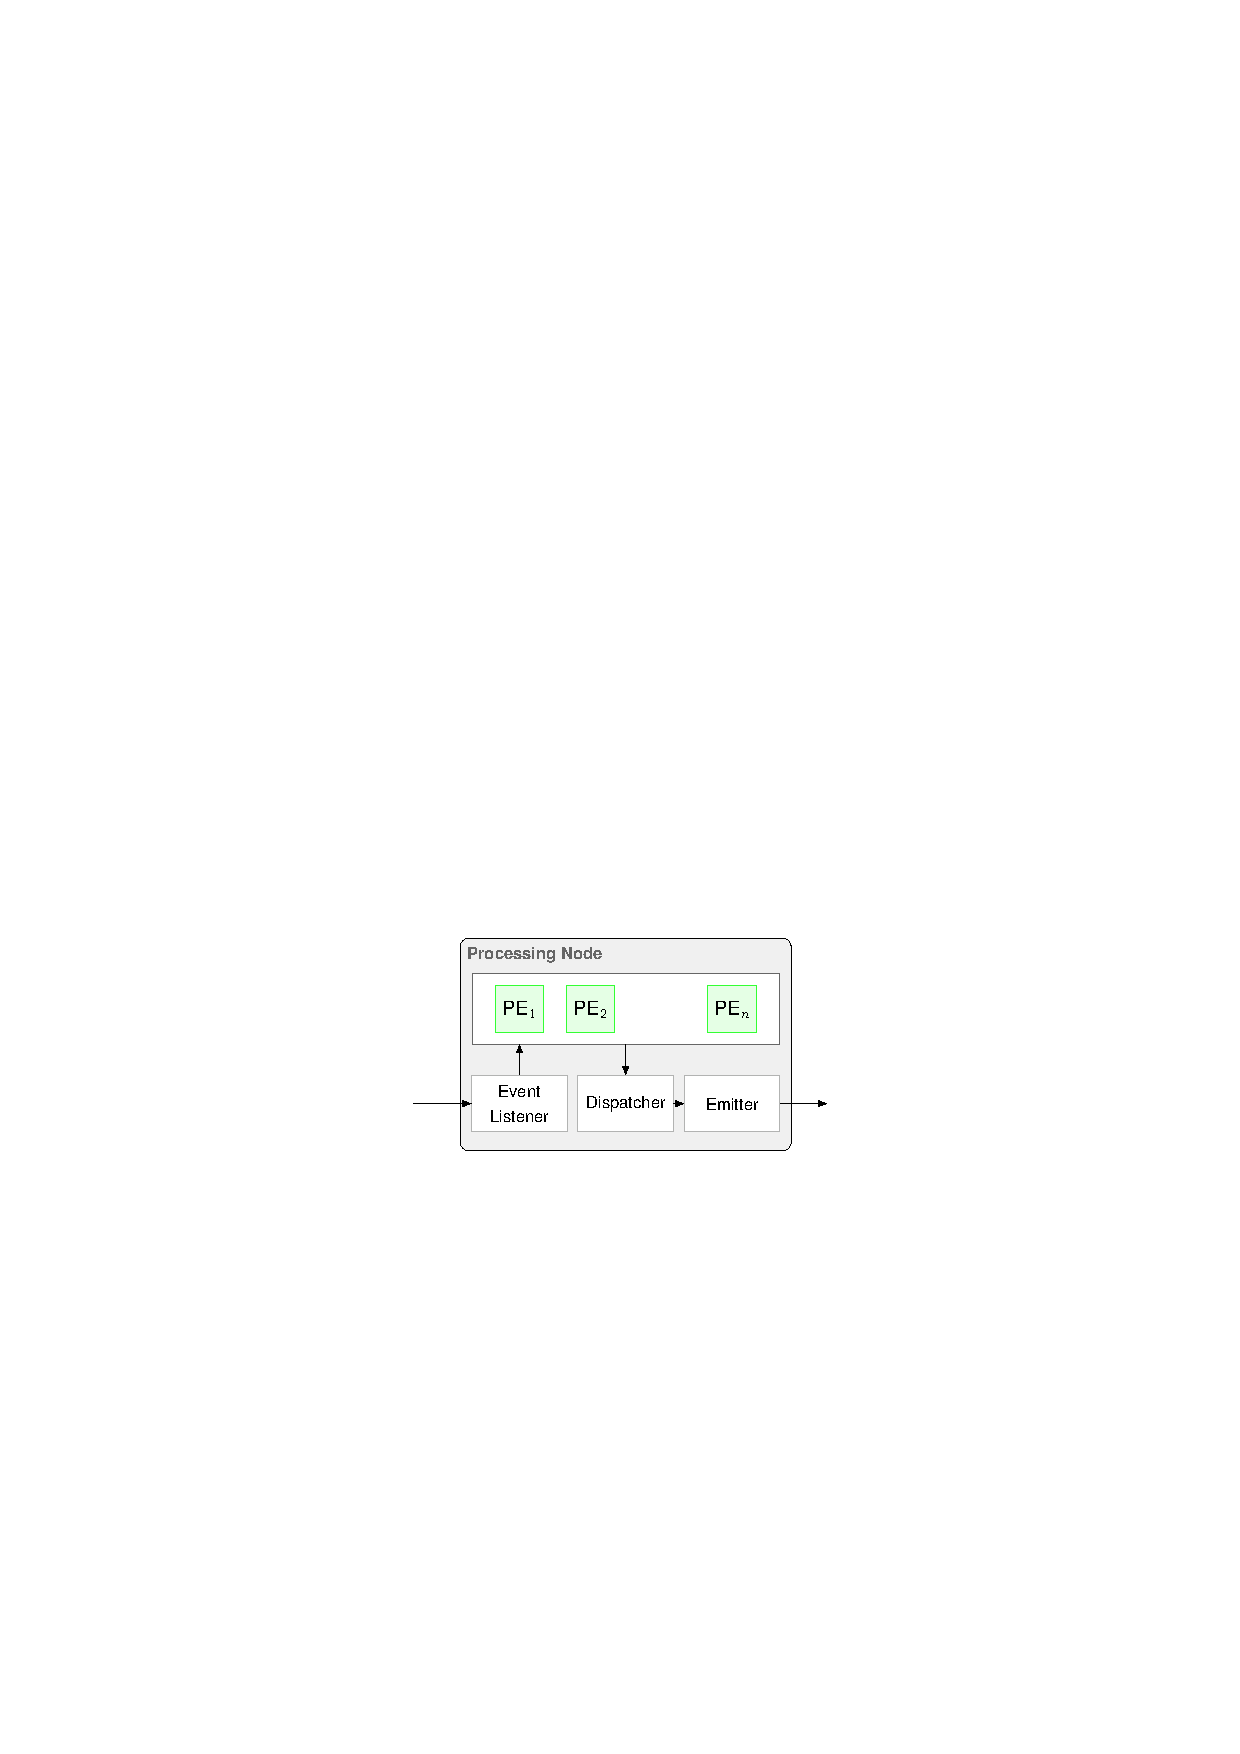
\includegraphics[width=0.6\textwidth]{images/s4/structure.pdf}
	\caption[Structure of an S4 processing node]{Structure of an S4 processing node \cite{bockermann2014survey}}
	\label{fig:s4_structure}
\end{figure}

Regarding fault tolerance, S4 detects node failures using Zookeeper and reassign tasks to other nodes \cite{bockermann2014survey}, passive stand-by processing nodes to be exact, a technique called \emph{lossy failover} \cite{kamburugamuvesurvey}. The message semantics guarantees only \emph{at-most-once} processing, which means that events may be lost as no buffering or acknowledgement of events is provided (\emph{gap recovery}).

S4 does however have a state management mechanism that periodically checkpoints the state of PEs to a backend storage. In case of a failure the reassigned task will load the last checkpointed state.

\subsection{Spark Streaming}

Spark Streaming is a \emph{stateful} distributed stream processing system, part of the Apache Spark cluster computing framework. One key difference of this platform is the way it handles data streams, with events being processed in \emph{batches} of fixed time intervals instead of a \emph{record-at-a-time} \cite{spark2015docs}.

Batches are also treated as \emph{Resilient Distributed Datasets} (RDDs), a data structure that keeps data in memory and can be recovered without the need of replication. Instead it tracks the \emph{lineage graph} of operations applied in order to build it, something possible since the computations are deterministic \cite{zaharia2013discretized}.

In Spark Streaming streams are called \emph{D-Streams} (discretized streams), sequences of immutable and partitioned RDDs, with deterministic operations applied at them to create new D-Streams.

The framework follows the \emph{monad} programming model. The API provides functionality for reading input data from outside the system in order to create the initial D-Stream. There are two types of operations that can be applied to D-Streams: \emph{transformations} and \emph{output operations}. The framework provides the basic \emph{stateless} operations commonly seen in batch processing frameworks (and functional programming languages), in addition to \emph{windowing} operations, \emph{incremental aggregations} and \emph{state tracking}.

An application is what can be called a \emph{D-Stream Graph}, analogous to the dataflow graph discussed in Section \ref{sec:esp:concepts}. At each batch interval the RDD graph is computed from the D-Stream graph, each output operation will create a Spark action which will in turn create a Spark job to compute the interval.

\begin{figure}[!ht]
	\centering
	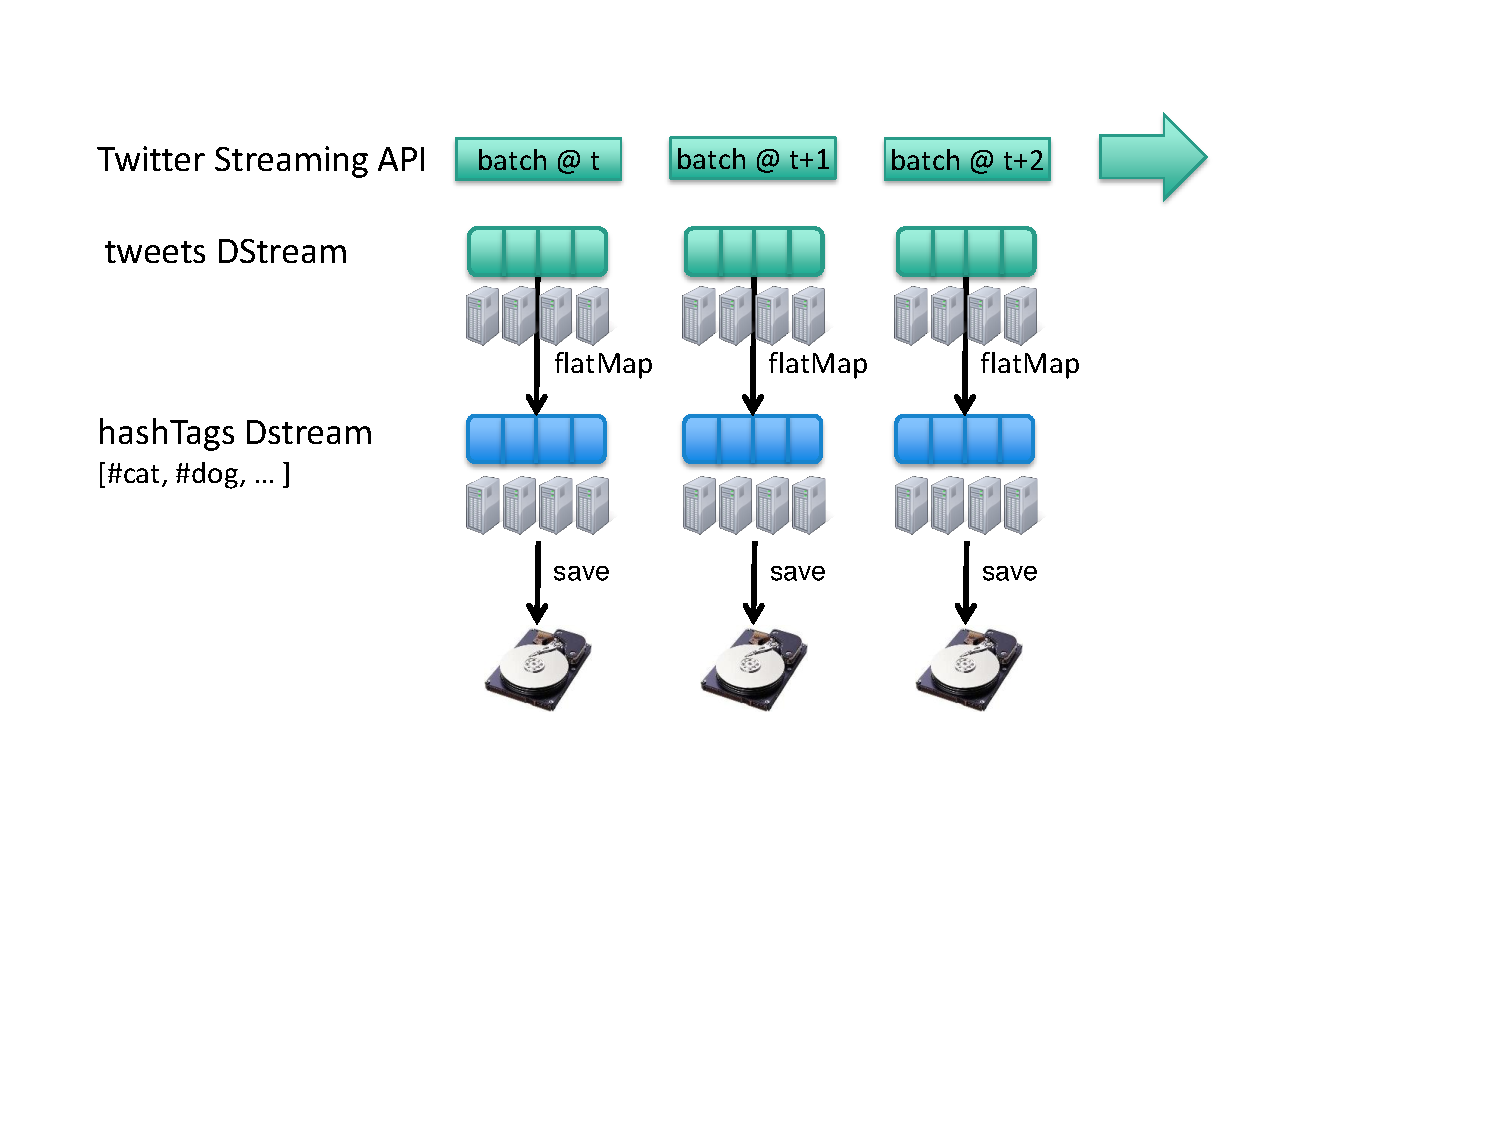
\includegraphics[width=0.6\textwidth]{images/spark/example.pdf}
	\caption[Example of application in Spark Streaming]{Example of application in Spark Streaming that reads input data from Twitter Streaming API, extract the hashtags and saves them on an external storage (e.g. HDFS).}
	\label{fig:s4_structure}
\end{figure}

Spark Streaming can recover from failures by using RDDs. The input data is replicated in memory and in case of a failure an RDD partition can be recomputed by applying the transformations that built it to the input data. It also checkpoints the state of RDDs periodically to an external storage (e.g. HDFS), and the recovery can be performed in parallel.

\begin{figure}[ht]
    \centering
    \subfigure[Components \cite{zaharia2013discretized}]{%
        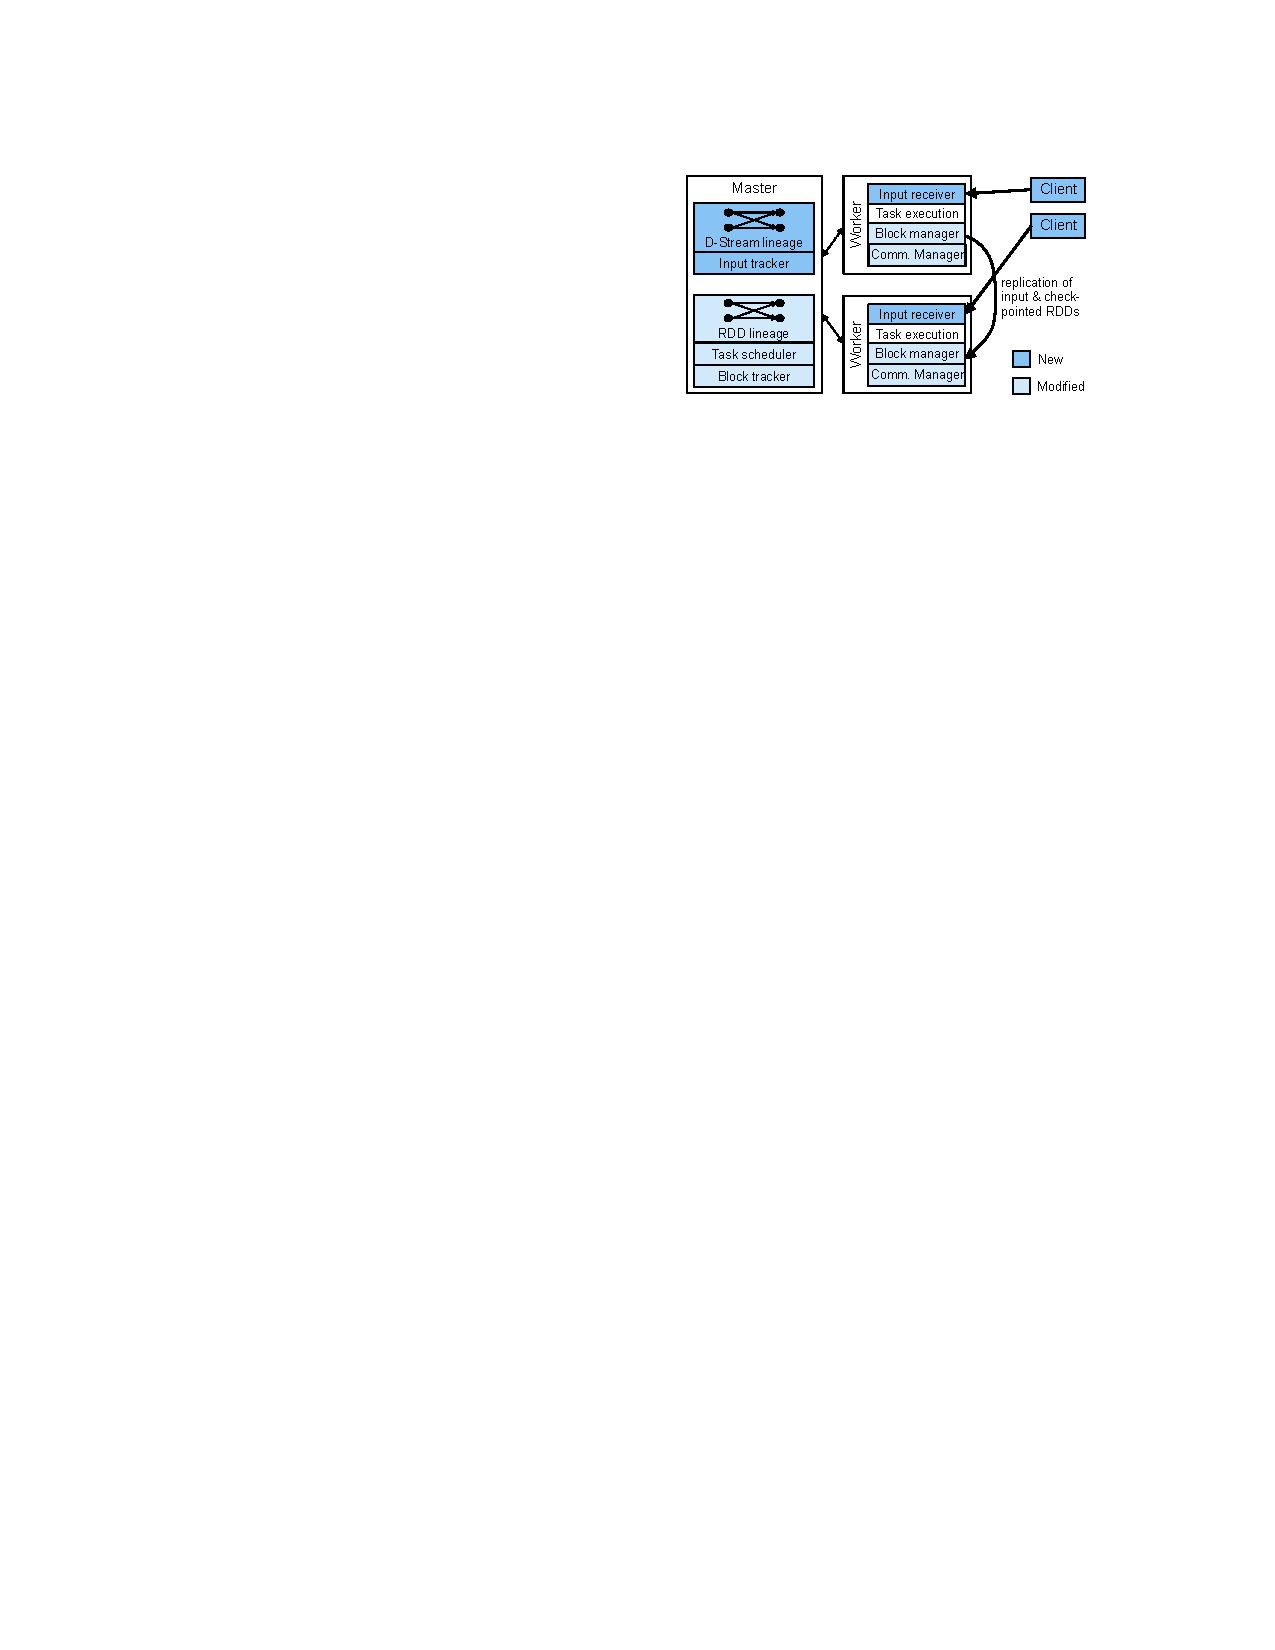
\includegraphics[width=0.4\textwidth]{images/spark/architecture.pdf}
        \label{fig:spark_architecture_components}}
    \quad
    \subfigure[Data Reception \cite{das2013spark}]{%
        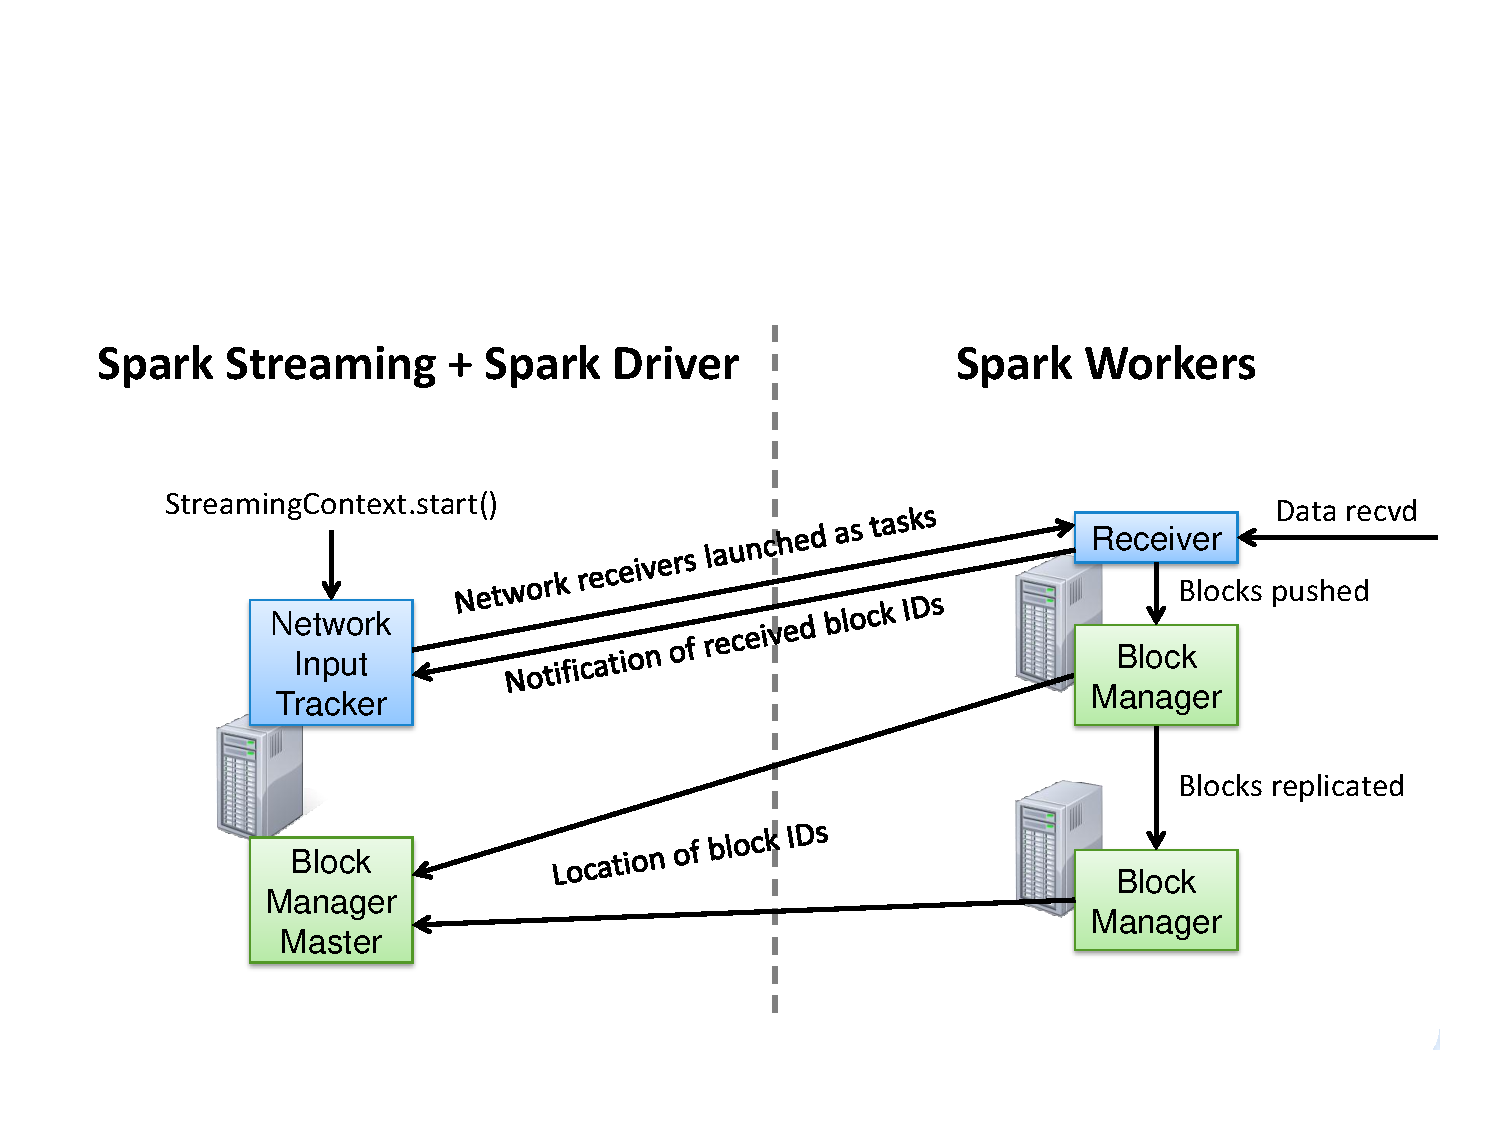
\includegraphics[width=0.4\textwidth]{images/spark/execution_model.pdf}
        \label{fig:spark_architecture_exec_model}}
    \subfigure[Job Scheduling \cite{das2013spark}]{%
        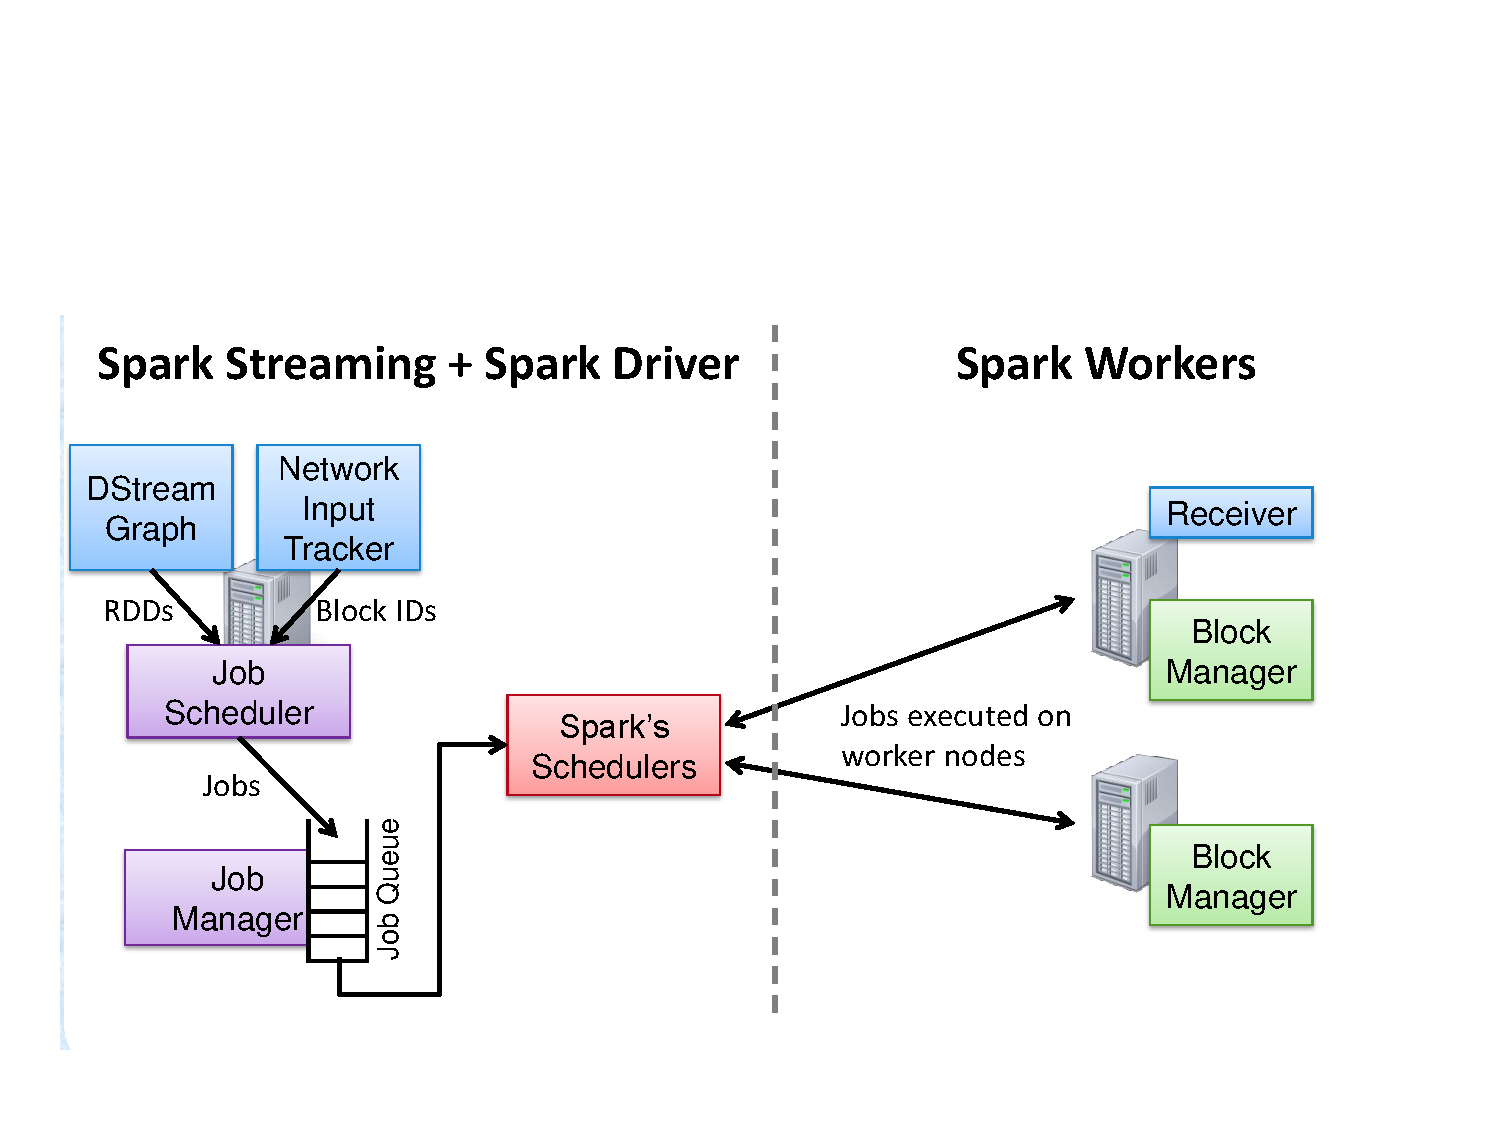
\includegraphics[width=0.4\textwidth]{images/spark/scheduling.pdf}
        \label{fig:spark_architecture_scheduling}}
    \quad
    \caption{Spark Components}
    \label{fig:spark_architecture}
\end{figure}

Its architecture (Figure \ref{fig:spark_architecture} \subref{fig:spark_architecture_components}) consists of three main components: a \textbf{master} that manages the lineage graph of D-Streams and schedules tasks to compute new RDD partitions; the \textbf{worker nodes} that receive data, store the partitions of input and computed RDDs and execute tasks; and the \textbf{client library} that sends the data into the system.

In Spark the component responsible for receiving data from the network is the \emph{Network Receiver} (Figure \ref{fig:spark_architecture} \subref{fig:spark_architecture_exec_model}), when it receives data it launches tasks in the workers in order for transfer it to them. The \emph{Receiver} then push the data blocks to the \emph{Block Manager}, the block will also be replicated and the Receiver will notify the master that the blocks have been received and send to the \emph{Block Manager Master} the location of the block IDs.

The \emph{Job Scheduler} (Figure \ref{fig:spark_architecture} \subref{fig:spark_architecture_scheduling}) periodically queries the D-Stream graph in order to create the jobs for the received data for the batch intervals. These jobs are stored in a queue by the \emph{Job Manager}, also responsible for sending them to the Spark Scheduler for execution in the worker nodes.


\subsection{Samza}

Samza is a framework for distributed stream processing built around Kafka. In Samza an operator is a \emph{job}, it can subscribe and publish to one or more streams. The parallelism is defined by the number of partitions of the Kafka's topic that the job subscribes to (if multiple topics, the one with more partitions). 

A job is then broken down into \emph{tasks}, each one responsible for consuming data from one or more partitions, that operates independently of each other \cite{ramesh2015samza}. These tasks will be executed by \emph{Task Runners}.

As a job is the equivalent of a single operator, more complex data flows can be created by submitting more jobs to Samza, connected only by their input and output streams. This particular characteristic makes it possible to change a data flow without stopping the application.

\begin{figure}[!ht]
	\centering
	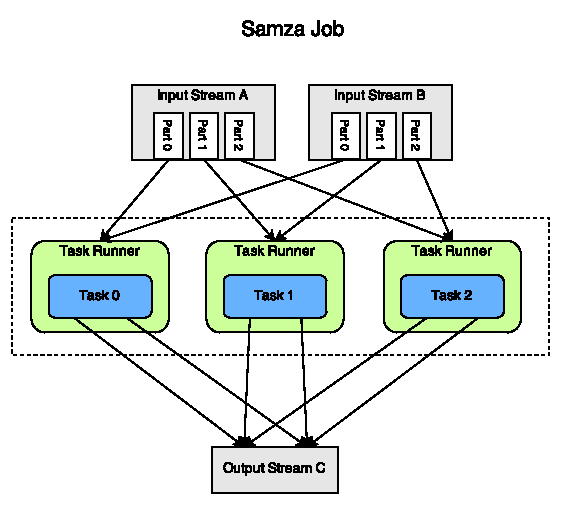
\includegraphics[width=0.6\textwidth]{images/samza/job_2.pdf}
	\caption[A Samza Job executing a user-defined task]{A Samza Job executing a user-defined task with two input streams, each with two partitions.}
	\label{fig:samza_job_execution}
\end{figure}

The architecture of Samza is divided in three layers: \emph{processing}, \emph{execution} and \emph{streaming}. While Samza is responsible for processing the data, the execution (distribution, scheduling and coordination) of tasks lies upon a \emph{cluster manager} such as Apache Mesos or Apache YARN \cite{ramesh2015samza}. Samza places the \emph{Task Runners} inside the containers of the cluster manager in order for them to be executed \cite{bockermann2014survey}.

Besides the \emph{execution} layer, the \emph{streaming} layer is also abstracted from Samza, giving the possibility to plug other systems for the transportation of messages, such as HDFS or a database.

When using Kafka as the streaming layer, Samza can guarantee \emph{at-least-once} message delivery using \emph{upstream backup} techniques. When a task fails another one takes over the topic partition, which is stored in disk, and continues consuming messages from the last offset checkpointed by the task that failed \cite{kamburugamuvesurvey}.

Another advantage of Samza lies in the fact that jobs are independent of each other, thus providing isolation in the event of a failure. And by using Kakfa it also means that an upstream job doesn't need to stop producing messages until the failed job is restarted \cite{ramesh2015samza}.

\begin{figure}[!ht]
	\centering
	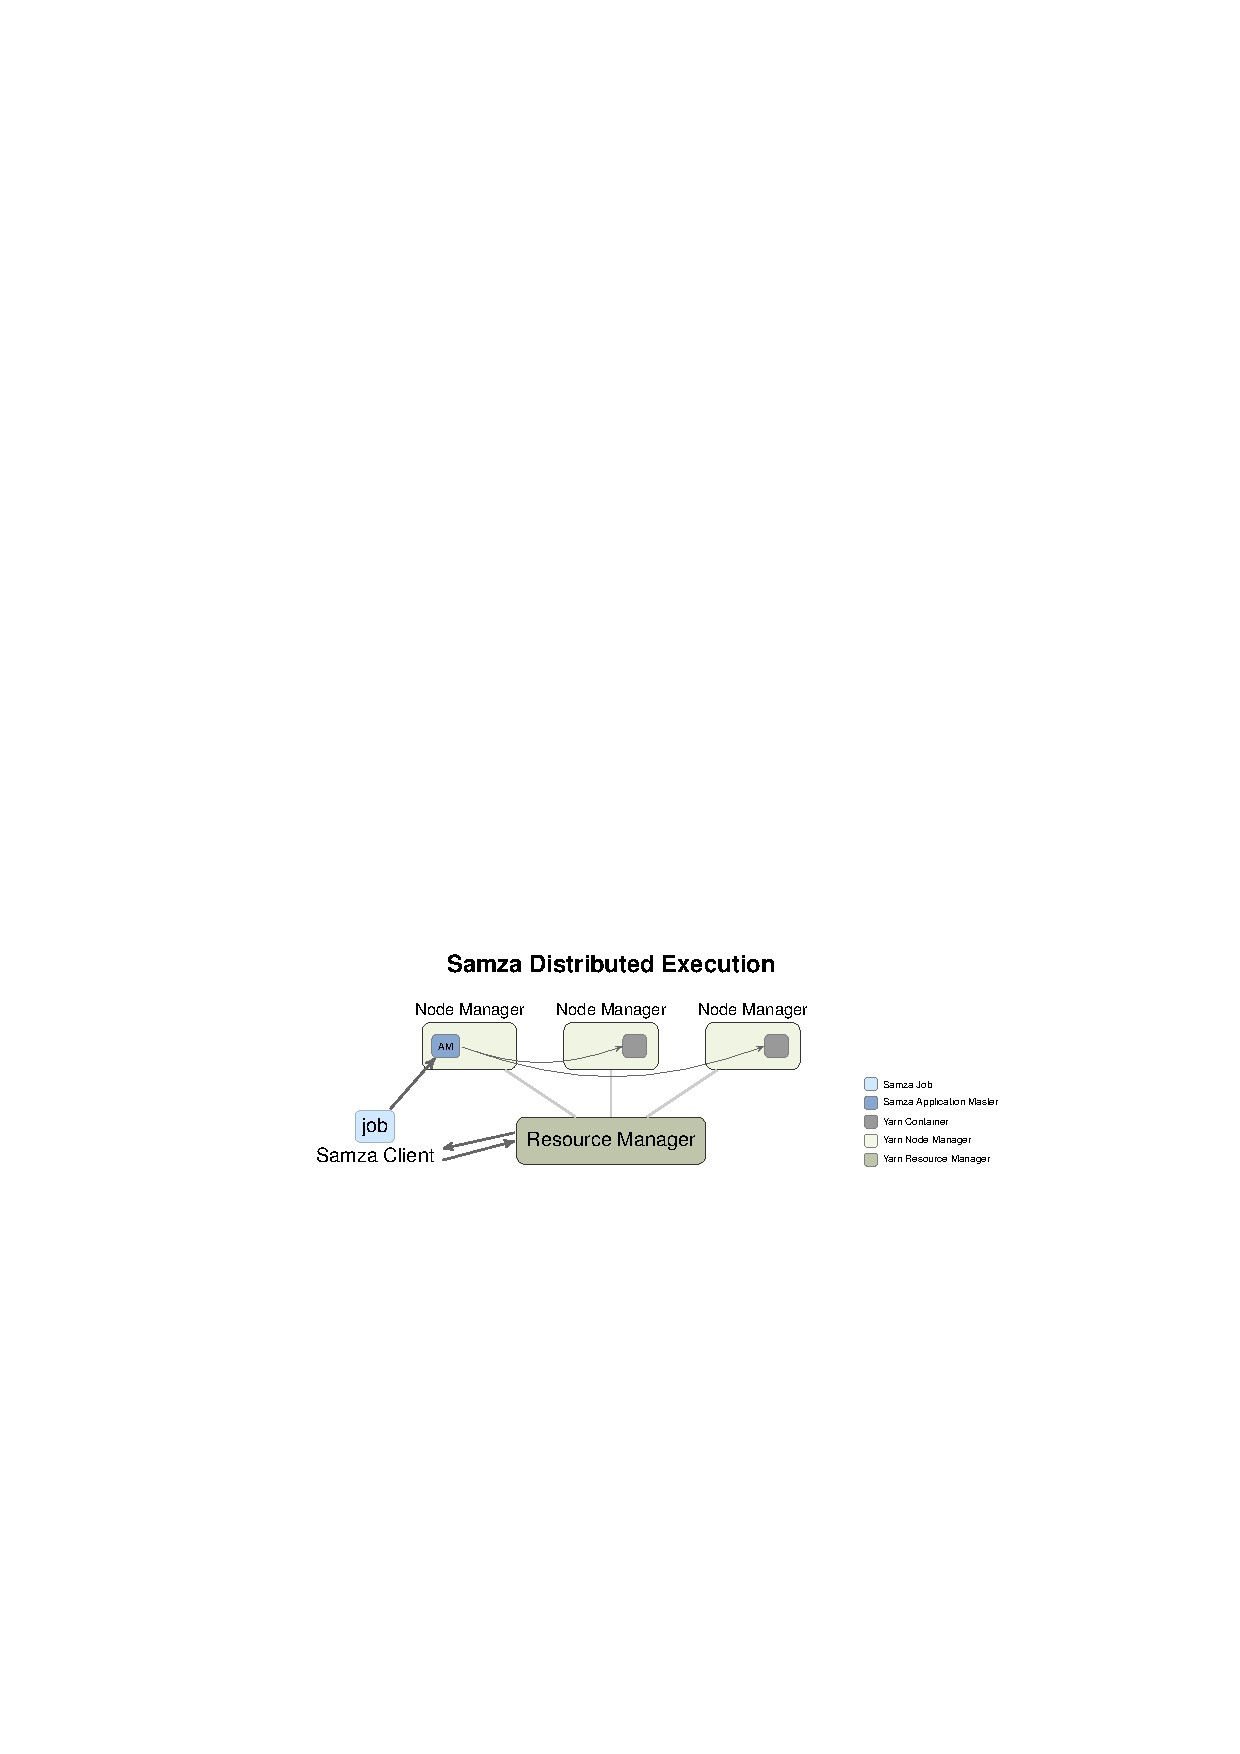
\includegraphics[width=0.6\textwidth]{images/samza/architecture.pdf}
	\caption[Architecture of the Samza job execution on Hadoop YARN]{Architecture of the Samza job execution on Hadoop YARN \cite{bockermann2014survey}}
	\label{fig:samza_architecture}
\end{figure}

Regarding state management, Samza provides its own data-store (e.g. LevelDB or RocksDB) located in the same machine as the task in order to give a better read/write performance. It also relies on Kafka for replication of the state in the form of a \emph{change-log} stream. In case of a failure the new task can consume the messages from the \emph{change-log} stream in order to restore its state.

\subsection{Comparison}

In this section the platforms described above will be compared regarding their main characteristics. These platforms were selected in particular because they all belong to the third generation of SPSs, they are focused on processing large volumes of data ("Big Data"), they are all open source, which means that the details under the hood are available for study, and they have gathered momentum over the last few years (with exception of S4, which is slowly fading away from the market).

Table \ref{table:sps_comparison} summarizes the main characteristics of these platforms. These characteristics were found in the documentation of the respective platforms and in previous works \cite{bockermann2014survey, gradvohl2014comparing, kamburugamuvesurvey} that compared some of these platforms.

Most of the characteristics used for the comparison have been described in Section \ref{sec:esp:concepts}, considering that they are some of the building blocks of SPSs. Others however, are more specific or technical and as such they will be detailed in the following paragraphs.

The \textbf{distributed cluster} characteristic refers to the support of the platform for working in multiple computers as a distributed system, something that all the platforms compared have. Directly related to the previous characteristic, the \textbf{stream partitioning} represents the data partitioning features of the platforms, something necessary in order to parallelize SPAs among nodes in a cluster. The difference is the way the partitioning is implemented, and among these platforms Storm is the one with the widest range of options.

\textbf{Rebalacing} is the capacity to rebalance the executing processes among the computing nodes in order to cope with changes in the load. Together with a \textbf{dynamic cluster}, i.e. the ability to add new nodes to a running cluster, it is possible to scale an application as it requires more resources in order to honor the application's QoS requirements.

\emph{Dynamic graph} is the ability to make changes in an application (add or remove operators) without having to restart it.

Regarding the communication characteristics, the \textbf{message system} refers to the middleware or library used to create the channels between the components of an application, whereas the \textbf{data mobility} indicates if the components control the flow rate (pull) of messages or not (push).

The \textbf{delivery guarantees} on the other hand are closely related to the \textbf{fault tolerance} mechanisms implemented by the platforms, topic approached in Section \ref{sec:esp:fault_tolerance}. The values for the available guarantees are: EO (exactly once), AMO (at most once), ALO (at least once), OO (out of order).

\begin{table}[t]
\begin{center}
	\footnotesize
	\begin{tabular}{ | p{2.5cm} | p{2cm} | p{2.5cm} | p{2.5cm} | p{2cm} | p{2cm} |}
   		\hline
		\textbf{Name}                    & Storm & Storm Trident & Spark Streaming & Samza & S4 \\\hline
		\textbf{Year}                    & 2011 & 2012 & 2013 & 2013 & 2010 \\\hline
        \textbf{Creator}                 & BackType & Apache & AMPLab, UC Berkeley & LinkedIn & Yahoo! \\\hline
        \textbf{Maintainer}              & Apache & Apache & Apache & Apache & Apache \\\hline
        \textbf{Category}                & Open Source & Open Source & Open Source & Open Source & Open Source \\\hline
        \textbf{Processing Model}        & record-at-a-time & micro-batches & micro-batches & record-at-a-time & record-at-a-time \\\hline
        \textbf{Programming Model}       & DAG & DAG & Monad & DAG & Actors \\\hline
        
        \textbf{Stream Partitioning}     & Yes & Yes & Yes & Yes & Yes \\\hline
        \textbf{Distributed Cluster}     & Yes & Yes & Yes & Yes & Yes \\\hline
        \textbf{Rebalancing}             & Yes & Yes & No \cite{tomassi2014spark} & No & Yes \\\hline
        \textbf{Dynamic Cluster}         & Yes & Yes & Yes & Yes & No \\\hline
        
        \textbf{Resource Management}     & Standalone, YARN, Mesos & Standalone, YARN, Mesos & Standalone, YARN, Mesos & YARN, Mesos & Standalone \\\hline
        \textbf{Coordination}            & Zookeeper & Zookeeper & Built-In & Built-In & Zookeeper \\\hline
        
        \textbf{Programming Language}    & Java, Any (w/ Thrift) &  & Java, Scala, Python & JVM-languages & Java \\\hline
        \textbf{Implementation Language} & Java, Clojure & Java & Scala, Java & Scala, Java & Java, Groovy \\\hline
        
        \textbf{Built-in Operators}      & No & Yes & Yes & No & No \\\hline
        \textbf{Deterministic}           & - & - & Yes & - & - \\\hline
        
        \textbf{Message System}          & Netty & Netty & Netty, Akka & Kafka & Netty \\\hline
        \textbf{Data Mobility}\cite{kamburugamuvesurvey}          & Pull & Pull &  & Pull & Push \\\hline
        \textbf{Delivery Guarantees}\cite{bockermann2014survey}    & AMO, ALO & EO, AMO, ALO & EO & EO & AMO \\\hline
        \textbf{Fault Tolerance}\cite{gradvohl2014comparing}         & Rollback recovery using upstream backup &  & Coordinated periodic checkpoint, replication, parallel recovery & Rollback recovery \cite{kamburugamuvesurvey}  & Uncoordinated periodic checkpoint \\\hline
        \textbf{Dynamic Graph}           & No & No &  & Yes & Yes \\\hline
        \textbf{Persistent State}        & No & Yes & Yes & Yes & Yes \\\hline
        
	\end{tabular}
	%\vspace{5px}
	\begin{flushleft}
	\end{flushleft}
	\caption{SPSs comparison}
	\label{table:sps_comparison}
\end{center}
\end{table}

\subsection{Other Platforms}

In the last three years a lot of platforms have been created or gained a lot of attention. Among those Flink and its streaming module is one of the most prominent. It is an open source distributed batch and stream processing platform. It's streaming engine has the record-at-a-time processing model with exactly-once delivery guarantees and support for state persistence.

Among the open-source platforms that appeared in the last few of years are: Apache Apex, a YARN-native platform that unifies batch and stream processing; Apache Beam, a programming model for building and executing batch and stream applications in a number of supported platforms (Apex, Spark, Flink and Google Cloud Dataflow); Apache Gearpump, a event/message based stream processing engine based on Akka; Apache Ignite, a streaming and continuous event processing engine with focus on scalability and fault-tolerance; hazelcast-jet, a distributed data processing engine that works on top of Hazelcast; Heron, a distributed stream processing engine created by Twitter to replace Storm, with a fully compatible API.

\section{Performance Evaluation}
\label{sec:esp:performance_evaluation}

Of interest of this work are benchmarks specifically designed for SPSs, comparisons between SPSs, performance tests of new SPSs, use cases of applications that employ an SPS and perform some experiments to evaluate it, sometimes comparing against a traditional solution; and benchmarks and frameworks from CEP systems, due to the similarities that exist between these two areas.

In the end, in Section \ref{subsec:esp:metrics}, a summary of the metrics employed by each of the related works is given, as a way to find a consensus.

\subsection{Benchmarks}
\label{subsec:esp:benchmarks}

The first benchmark designed specifically for stream processing systems that can be found in the literature is the Linear Road Benchmark \cite{arasu2004linear}, adopted by the Aurora \cite{abadi2003aurora} and STREAM \cite{arasu2004stream} systems. It simulates a toll system in a fictitious city with the purpose of calculating the toll value based on traffic jam and accident proximity, charging drivers greater values when there's more congestion as a way to discourage them from using the roads. In this simulation there are express ways composed of four lanes, with vehicles reporting their position every 30 seconds and accidents happening in random locations every 20 minutes. The purpose of the benchmark is to determinate the maximum L factor (number of express ways) that a system can process without violating the response time and precision requirements. The queries defined by the benchmark are: accident detection, traffic congestion measurement, toll calculation and historical queries. At the end of the paper a comparison between a relational DBMS and Aurora is presented, with a measured L factor of 0.5 and 2.5, respectively.

%Besides the Linear Road Benchmark, the only benchmarks found in the literature that are designed for stream processing are aimed at very specific cases, as is the case of PLR \cite{karachi2012plr} which is an extension of the Linear Road for probabilistic DSMSs, and the SRBench \cite{zhang2012srbench} that defines a set of queries for the comparison of Streaming RDF/SPARQL (strRS) engines.

Besides the Linear Road Benchmark, there are benchmarks for SPSs that are aimed at very specific cases, as is the case of PLR \cite{karachi2012plr} which is an extension of the Linear Road for probabilistic DSMSs, and the SRBench \cite{zhang2012srbench} that defines a set of queries for the comparison of Streaming RDF/SPARQL (strRS) engines.

%Another benchmark (and framework) aimed at comparing Streaming RDF (also known as Linked Stream Data or LSD) engines is the LS-Bench \cite{le2012linked}. The authors have built a framework for simulating the generation of data from social networks (SNs), running the engines and analysing the output. The benchmark is composed of twelve queries with increasing levels of complexity in order to verify how many queries an engine supports. Besides analysing the functionalities supported by an engine, the benchmark also tests the correctness of the results produced and the performance of the engine, the last one is accomplished by setting the input rate at its maximum and observing the behavior of the engine. The performance tests also evaluate the scalability of engines using the static data size and the number of simultaneous queries as factors, and the throughput as metric.

% StreamBench

The first benchmark suite for the 3rd generation of SPSs is StreamBench \cite{lu2014stream}. It proposes a set of seven applications for the workload, based on three dimensions of requirements for stream processing: \emph{data type}, \emph{workload complexity} and \emph{use of historical data}. The benchmark also defines four aspects that are going to be measured: \emph{performance}, with the input rate at its maximum with four input scales (5M, 10M, 20M and 50M); \emph{multi-recipient performance}, where the input scale is fixed but the number of nodes in the cluster that receive the input data varies (single node, half of the nodes and all nodes of the cluster); \emph{fault tolerance}, with half of the nodes as recipients, it consists on failing one non-recipient node and measuring the performance under failure and comparing to a failure free experiment; \emph{durability}, uses only one application with 10K and 1M records per minute during 2 days, and measures the percentage of available time of the framework.

The applications that compose the benchmark suite are: \emph{identity}, \emph{sample}, \emph{projection}, \emph{grep}, \emph{word count}, \emph{distinct count} and \emph{statistics}. Six of them work with text data types and one with numeric data type, four of them have only a single operator and are stateless. One shortcoming of this benchmark suite is that all applications are synthetic, leaving aside more complex operations and communication patterns that only occur with more complex data flow graphs. It's worth noting that the authors acknowledge this fact.

The datasets used by the benchmark suite are from real world scenarios and they use them as seed for data generation. The seed data should be pre-loaded in memory in order to increase the performance as the data generation speed should be superior to the data consumption. The generated data, according to the proposed architecture, is feeded into a message system, decoupling the data generation from data consumption. It is also necessary that the message system should have a serving speed superior from the consumption speed. The authors claim that even if the SPSs could achieve greater throughput without a message system, by being the common data transport for all experiments it results in a fair comparison.

As most of the works below, they chose the \textbf{average} \emph{throughput} and \emph{latency} as main metrics, and the penalties incurred from failures in this two metrics. They have done experiments to compare Storm and Spark Streaming in a cluster of 6 nodes, using Apache Kafka as the message system in a cluster of 6 nodes, with 5 of them as brokers. They fail, however, to present the standard deviation of the results measured, something essential for the comparison of systems known for their high variability in latency and throughput.


% Yahoo Streaming Benchmark \cite{yahoo2015bench}
% Ad campaign events processing application
% For Storm, Spark, Flink and Apache Apex
Another benchmark for SPSs was Yahoo Streaming Benchmark \cite{yahoo2015bench}, composed of an Ad campaign stream application and implementations for Storm, Spark, Flink and Apex systems. They analyze the throughput and 99th percentile of latency on those platforms with their default set-up configurations. Results showed that Storm had a great performance and a throughput almost as good as Flink and with some optimizations it could achieve an even better performance.


% BigDataBench \cite{wang2014bigdatabench}
% BigDataBench has five applications for the evaluation of streaming systems: grep, search, rolling top words, k-means and collaborative filtering (for e-commerce).
A later work on benchmarking Big Data systems is BigDataBench \cite{wang2014bigdatabench}, with a wide range of applications from multiple areas. It also has a subset of five micro-benchmarks specific for streaming systems: \textit{grep}, \textit{search}, \textit{rolling top words}, \textit{k-means} and \textit{collaborative filtering} (for e-commerce).

It provides the specification of all benchmark applications as well as the data inputs, but it is not a framework in the sense that it does not provide an API that can be extended for building new benchmarks. The micro-benchmarks have been implemented for JStorm and Spark.

% micro-benchmark, which platforms? has framework?


% StreamBench \cite{wang2016stream}
% StreamBench defines an extensible framework for SPS evaluation, but the applications need to be rewritten for each new platform that is going to be tested. Furthermore, the benchmark only defines three applications: AdvClick, for clickstream analysis with correlation between ads and clicks on those ads; WordCount; and K-Means, applied to a stream of points with a pre-defined set of centroids. Those three applications are evaluated on Storm, Spark and Flink, using latency and throughput as metrics.
% covers only micro-benchmarks, not real world and complex applications, inputs are also not realistic

Another work specific for SPSs is StreamBench \cite{wang2016stream} (not the same as \cite{lu2014stream}), an extensible framework for the evaluation of these systems. The benchmark defines three micro-benchmarks: \textbf{AdvClick}, for clickstream analysis with correlation between ads and clicks on those ads; \textbf{WordCount}; and \textbf{K-Means}, applied to a stream of points with a pre-defined set of centroids.

The benchmark provides implementations of those applications for Storm, Spark and Flink, using the latency and throughput as evaluation metrics. One downside of the framework is the fact that applications need to be implemented for each platform separately. In addition, these applications do not represent real world and complex applications, and they don't use realistic inputs.


% \cite{shukla2017riotbench}
% RIoTBench

A different approach is taken by RIoTBench \cite{shukla2017riotbench}, they focus on IoT (Internet of Things) applications, defining 27 tasks that can be combined to create micro-benchmarks (they define four of such). They have evaluated the benchmark against Storm regarding the throughput, latency, resource usage and a new metric called \textit{jitter}, which tracks the variation between the expected and actual output throughput.


% HiBench \cite{huang2010hibench}
% Defines four micro-benchmarks: wordcount, fixed window, identity and repartition.
% For Storm, Spark and Flink

Another benchmark for Big Data systems is HiBench \cite{huang2010hibench}, originally it defined a set of synthetic, micro-benchmarks and real world applications for MapReduce (batch processing), specifically Hadoop. They used the benchmark to characterize Hadoop in terms of speed, throughput, bandwidth of HDFS, resource utilization and data access patterns.

Only recently they have added support for streaming platforms, defining four micro-benchmarks: \textit{wordcount}, \textit{fixed window}, \textit{identity} and \textit{repartition}. Those applications have been implemented for Storm, Spark and Flink.


\subsection{SPS Comparisons}

In a study conducted in 2011 \cite{dayarathna2011performance} the scalability of Apache S4 and System S is compared using three applications (CDR, VWAP and trending topics) plus a micro-benchmark. They measure the throughput with 1, 2, 4, 6, 8 and 12 nodes. In all scenarios System S is superior, but the authors don't disclose if the throughput is the average, the maximum or minimum, or some percentile.

In a latter work by the same authors \cite{dayarathna2013performance}, they evaluate the performance of Apache S4, System S and Esper using the same applications as in their previous work analysis, beyond the throughput, the resource usage of these systems. The authors took care of modifying the applications in order to give a fair comparison between the systems. The throughput was measured in two ways: for Apache S4 and Esper they measured the time required to process a certain number of tuples, while in System S the throughput was computed over the time to process the whole dataset. The experiments were repeated three times for each combination of factors, and the average was used to calculate the throughput. The CPU, memory and network usages are retrieved using Nmon and Oprofiler.

Although the last work is recent, it left out Storm, which is one of the most popular SPS. At that time other systems, such as Spark Streaming, Samza and Dempsy were just in its infancy, but it means that there is no comparison between these systems in the literature, nor even in white papers or technical reports.

\subsection{SPS Performance Tests}

In the Spark Streaming platform \cite{zaharia2012discretized} they measure the maximum throughput achievable of the system with 1s and 2s of maximum latency for different cluster sizes. They also introduce node failures and measure the processing time for each job, before and after the failure.

In an evaluation of the performance of Apache S4 \cite{chauhan2012performance} a single application is used to observe its scalability, resource usage and fault tolerance. For the scalability analysis they use as factors the number of nodes in the cluster (1 to 3), data size (10 and 100 megabytes), input rate (500 and 1000 events/sec), and number of keys. The metrics are the total number of events processed (50k times number of keys) and the number of events lost. They do not use runtime as a metric because an under provisioned setup would lead to high tuple loss and small runtimes, giving the false impression that using one node is better than two or more. The resource usage is depicted for each node of the cluster with the CPU and memory usage, while the network usage is summarized for the whole cluster and measured in packets per second. The experiments that evaluate the fault tolerance of Apache S4 were conducted by killing one (in a 2-node and 3-node cluster) and two (in a 3-node cluster) nodes leading, as expected, to a reduction in throughput, overwhelming the remaining nodes and thus leading to higher tuple losses.

For MillWheel \cite{akidau2013millwheel}, a distributed and fault tolerant SPS developed at Google, the main metric used to evaluate it is the latency. Regarding its scalability, they look at the median, 95th and 99th percentiles. Results show that while the latency median remains almost unchanged, the tail gets longer.

Another distributed SPS called TimeStream \cite{qian2013timestream} is evaluated regarding its scalability, fault tolerance, consistency and adaptability to load dynamics. TimeStream packs events into batches for transportation, by varying the batch size they measure the maximum throughput and latency with a distinct count application. They pick five batch sizes and measure the throughput and latency with different number of computing nodes and compare it with Apache Storm. In a sentiment analysis application they use a dataset of 1.2 billion tweets, feeding the system at a rate of 600 tweets/s in average, with a peak of 2,000 tweets/s. To evaluate the fault tolerance of TimeStream the authors use the same two applications. With the distinct count they only inject a failure in one of the computing nodes and observe the recovery time for different window sizes and checkpointing intervals. For the sentiment analysis application they inject failures by selecting operators that form a chain in the DAG and killing one, three or the whole chain of operators and measuring the recovery time for each operator.

Fernandez et al \cite{castro2013integrating} implement a scalable SPS that exposes operator's internal state for checkpointing and backup purposes. For their experiment they use dedicated VM instances (with large RAM memory available) to emit the data streams and receive the results. Their system is able to scale as a result of an increasing input rate. The latencies observed were very skewed for the Linear Road Benchmark, as a result, the authors chose to use the 99th and 95th percentiles, besides the median. The authors also observe the time required for an operator to recover after the willful failure of the VM hosting the operator.

In the evaluation of Watershed \cite{de2011watershed}, a distributed SPS, a composed application for analysis of tweets is employed. The first experiment received data at a fixed rate of 10 tweets/s with the number of instances of one operator (stopwords remover) varying from 1 to 24. In this experiment only the throughput is measured over a runtime of 2 minutes. In a second experiment, 10M tweets are pushed to the system through a single instance of the collector operator (a spout), while the other operators of the application have the number of instances ranging from 1 to 7. This time they measure the execution time and calculate the speedup, but they don't repeat their experiments.

The largest experiment in terms of computing infrastructure for a SPS was done by \cite{gulisano2012streamcloud}. They used a cluster of 100 nodes to evaluate the scalability and elasticity of StreamCloud, the distributed SPS the authors had proposed. Their evaluation focus on the system's ability to harness the computing power available to process an increasing number of tuples. This ability is translated into the metrics of throughput and CPU usage. The authors also evaluate the throughput and CPU usage for fixed number of nodes, breaking down the metrics per operator. All the experiments were run three times, and the measurements were taken in the steady phase of the running time, which lasted at least 10 minutes.

These works were important in the selection of metrics and methodologies for the benchmark suite. There are some similarities among them, mainly regarding latency and throughput, although the way they have chosen to look to these metrics differs, some analyse the average while others prefer percentiles. This lack of consensus regarding the performance comparison of SPSs is one of the issues that is solved in our work.

Moreover, their experiments only use a few applications, greatly restricting the conclusions that can be drawn from them.


\subsection{Use Cases}

In a trend detection application using Storm \cite{chardonnens2013big}, the experiments were conducted using a cluster of six nodes. One of them was used solely for feeding data into Kafka. Kafka resided in two nodes, while Storm and Cassandra were running in four nodes. The authors analyzed the time required for processing 2TB of data from Twitter and Bitly with one up to three Storm supervisors.

Smit, Simmons and Litoiu \cite{smit2013distributed} propose and implement an architecture for real-time monitoring of cloud resources using Storm for processing streams of metrics, OpenTSDB for storing time-series results and Ganglia for monitoring the performance of the SPS. They compare the average latency of their solution, called MISURE, with Amazon CloudWatch. The average latency is measured over 100 samples, and it shows that MISURE has a latency of less than a second, while CloudWatch ranges between 90 and 300 seconds. The throughput of MISURE is displayed over a 15 minutes window (with 30 samples, 6 experiment runs and 5 samples per time interval) for 4, 8 and 32 computing cores. Over the whole running time (~450 minutes) increasing the number of cores by a factor of 8 incurred an increase in throughput by a factor of 6.85.


\subsection{Benchmarks and Frameworks for CEP Systems}

Heinze et al \cite{heinzeelastic} evaluates a query allocator on top of a distributed CEP engine. They measure the average system utilization with a fixed data rate, and varying data rates (bounded to a fixed range). They also measure the latency of the system along the time, but not directly, instead they use a metric called latency ratio, which is the ratio between the initial latency measured for the first ten seconds and the current latency.

In a correlated subject, Le-Phuoc et al \cite{le2012linked, le2013elastic} proposes a framework for the evaluation of LSD engines (Linked Stream Data, e.g. RDF stream data model). Their work includes a methodology for data generation, system testing and analysis of results. The tests defined by the framework fall into one of the three categories: functionality, correctness and performance tests. Functionalities are covered through queries of increasing complexity, and the results assert if the functionality is supported by the engine or not. The correctness tests evaluates the output of a query for all engines given the same input and configuration. In cases of mismatch between the outputs of different engines, a function for calculating the percentage of mismatch is employed. In the performance tests the main metric is throughput, but in the case of LSD engines, as the input rate increases the system may drop some tuples (load shedding), which could lead to wrong results. To circumvent this problem, the authors proposed the comparable maximum execution throughput.

Similar to the work described above, \cite{scharrenbach2013seven} gives a few insights into how to benchmark SFP (Semantic Flow Processing, i.e. LSD engines) systems. Of interest to this work is the three KPIs they have defined, they are: the response time, measured by the average, xth percentile or the maximum; maximum input throughput per unit of time; and other metrics including recall (reprocessing a lost tuple), precision and error rate.

%%

In 2007, Bizarro \cite{bizarro2007bicep} proposed the BiCEP project, a benchmark for CEP engines. The paper identified the categories of applications for CEP engines based on publications from a few conferences. It also defined a set of metrics: \emph{response time}; \emph{scalability}, broken down into \textbf{scale-up} (increase system and load), \textbf{speed-up} (increase system, maintain load) and \textbf{load-up} (maintain system, increase load); \emph{adaptivity}, which observes the behaviour of the engine in the face of changes in input rate, bursts in event arrival, system overloads and instability; \emph{computation sharing}, that evaluates the ability of the engine to have multiple queries running concurrently; \emph{precision} and \emph{recall}.

In continuation to the BiCEP project, Mendes, Bizarro and Marques \cite{mendes2008framework} developed a framework for the performance evaluation of CEP systems called FINCoS. The framework is language-agnostic, in the sense that it can be used with any CEP product; and workload-agnostic, enabling the use of any dataset and queries to evaluate a set of engines. The architecture of the framework is composed of drivers that simulate streams of events, sinks that are going to receive the output from the CEP engine, the controller used by the user to configure the environment (number of drivers and sinks, rate of events, number of machines), the adapters that translate the input and output between the CEP engine and the standard format, and the validators that check the output results as well as performance metrics (e.g. response time).

In a subsequent paper, the same authors put in practice their FINCoS framework \cite{mendes2009performance} using a set of micro-benchmarks to compare the performance of three CEP engines (Esper and other two commercial engines). Their benchmarks focus on simple operations (windowing, transformation, filtering, sorting, grouping, merging, join, pattern detection) using as factors the content of the dataset, window configurations, event rate, and number of queries (not all factors are used for a single benchmark). Just like the work by Gulisano et al \cite{gulisano2012streamcloud}, they also wait for the engine to warm-up before starting to measure the performance, for at least ten minutes, depending on the application. Experiments were repeated two times with the average being used. Most benchmarks use the throughput as their metric. In two cases were the size of the window is a factor they also measure the memory consumption with different input rates, window sizes and number of queries.

In another set of experiments their aim was to observe the engine's performance in the face of a burst. Like in the other experiments, the execution consisted of a warm-up period of one minute in which the input rate was increased to $\lambda$ such that the CPU utilization were around 75\%; in a steady phase of five minutes the rate was kept at the $\lambda$ rate; then during 10 seconds the injection rate was increased to $1.5\lambda$; and finally in a recovery phase the original input rate of $\lambda$ was restored. To characterize the performance of the engine the following metrics were introduced: maximum peak latency, the maximum latency during or immediately after the peak load; peak latency degradation ratio, the ratio between the 99th percentiles of the latency in the peak phase and in the steady phase; recovery time, which is the amount of time necessary for the engine to return to the latency level of the steady phase after a peak; and post-peak latency variation ratio, which is the ratio between the average latency after recovery and the steady phase.

%%

More recently, Wahl and Hollunder \cite{wahl2012performance} proposed an environment for the comparison of CEP engines, focusing on the interchangeability of engines, reproducibility and comparability of the test scenarios and automation of test execution and measurement. They defined three test scenarios: \emph{latency test}, which creates four events that are emitted to the CEP engine to create a complex event, and once this result event is received the latency is calculated; \emph{pollution test}, based on a defined CEP rule, events that fall into the rule are generated as well as events that don't, the rate of events is constant, but the number of irrelevant events is increased and the latency, CPU load and memory usage are monitored; and the \emph{load test} that increases the number of event emitters and observes the same parameters as the previous test.

%%

The most recent work on CEP benchmarking is CEPBen \cite{li2014cepben}, which is both a benchmark as well as a framework. One key difference of this work is that the smallest unit of data is not an event, but a batch of events. In practice there are three factors that can be changed in the workload: the number of batches, i.e. the size of the dataset; the size of the batch; and the interval between batches, i.e. the input rate. As most benchmarks, the CEPBen also uses as metrics the \emph{throughput}, subdivided into \emph{input} and \emph{output} throughput, and the \emph{response time}, i.e. (end-to-end) latency.

The authors of CEPBen define, instead of full-fledged applications, three groups of tests based on functionalities that are the building blocks of event processing: \emph{filtering}, \emph{transformation} and \emph{event pattern detection}. The factors that weigh in the experiments are, besides the workload, the number of query statements, as more statements means more operations that need to be performed for each event; the amount of historical events needed by the query, as it means more memory needs to be used to store these events; and of course, the hardware where the CEP engine is running.

The framework developed for running the benchmarks is very similar to previous works described here, with components for data generation and adaptation, event consumers that receive the results, and the components for monitoring, storing and analysing the engine's metrics. At the end of the paper they present a performance study using their benchmark with the Esper CEP engine.

\subsection{Metrics}
\label{subsec:esp:metrics}

The Table \ref{table:related_work_metrics} summarizes the metrics used by the works cited in the sections above. The metric that appears the most is scalability, followed by throughput and latency. The runtime is not so popular, mainly because SPAs in the real world usually don't have a limited execution time. The tuple loss and recovery time metrics are used in works that study the tolerance of SPSs to faults.

\begin{table*}[t]
\begin{center}
	\tiny
	\centering
	\begin{tabular}{ | l | c | c | c | >{\centering\arraybackslash}p{0.5cm} | c | >{\centering\arraybackslash}p{0.7cm} | >{\centering\arraybackslash}p{0.7cm} | >{\centering\arraybackslash}p{1.5cm} |}
   		\hline
        \textbf{Work} & \textbf{Scalability} & \textbf{Latency} & \textbf{Throughput} & \textbf{Tuple Loss} & \textbf{Runtime} & \textbf{Resource Usage} & \textbf{Recovery Time} & \textbf{Other} \\\hline
   		
		\cite{dayarathna2011performance} & \textbullet & & \textbullet & & & & & \\\hline
		\cite{dayarathna2013performance} & & & \textbullet & & & \textbullet & & \\\hline
		\cite{zaharia2012discretized} & \textbullet & & \textbullet & & \textbullet & & & \\\hline
		\cite{chauhan2012performance} & \textbullet & & \textbullet & \textbullet & & \textbullet & & \\\hline
		\cite{akidau2013millwheel} & \textbullet & \textbullet & & & & & & \\\hline
		\cite{qian2013timestream} & \textbullet & \textbullet & \textbullet & & & & \textbullet & \\\hline
		\cite{castro2013integrating} & & \textbullet & & & & & \textbullet & \\\hline
		\cite{de2011watershed} & & & \textbullet & & \textbullet & & & \\\hline
		\cite{gulisano2012streamcloud} & \textbullet & & \textbullet & & & \textbullet & & \\\hline
		\cite{chardonnens2013big} & & & & & \textbullet & & & \\\hline
		\cite{smit2013distributed} & \textbullet & \textbullet & \textbullet & & & & & \\\hline
		\cite{heinzeelastic} & & \textbullet & & & & & & \\\hline
		\cite{wahl2012performance} & & \textbullet & & & & \textbullet & & \\\hline
		\cite{le2012linked} & \textbullet & & \textbullet & & & & & \\\hline
		\cite{li2014cepben} & & \textbullet & \textbullet & & & & & \\\hline
		\cite{scharrenbach2013seven} & & \textbullet & \textbullet & & & & & recall, precision, error rate\\\hline
		\cite{bizarro2007bicep} & \textbullet & \textbullet & & & & & & adaptivity, precision, recall, computation sharing \\\hline
		\cite{lu2014stream} & \textbullet & \textbullet & \textbullet & & & & & \\\hline
		
		% new papers
		\cite{yahoo2015bench} &  & \textbullet & \textbullet & & & & & \\\hline
		\cite{wang2014bigdatabench} &  &  & \textbullet & & & & & \\\hline
		\cite{wang2016stream} &  & \textbullet & \textbullet & & & & & \\\hline
		\cite{shukla2017riotbench} &  & \textbullet & \textbullet & & & \textbullet & & jitter\\\hline
		\cite{huang2010hibench} &  &  & \textbullet & & \textbullet & \textbullet & & \\\hline
		
	\end{tabular}
	\vspace{5px}
	\caption{Related work metrics}
	\label{table:related_work_metrics}
\end{center}
\end{table*}

\subsection{Evaluation of the Existing Benchmarks}
\label{subsec:esp:evaluation_existing_benchmarks}

Of the benchmarks designed specifically for SPSs, described on Section \ref{subsec:esp:benchmarks}, they either focus on a single real-world application or they use a set of synthetic/micro-benchmark applications.

None of these works does a workload characterization of the applications that are part of the benchmark. This is essential in order to differentiate the applications that compose the benchmark and ensure that each application has a different set of behaviours.

These works also don't evaluate the relevance of those applications in the stream processing area. Having a diverse set of applications from multiple areas is important for the evaluation of the best platform for a type of application.

Another shortcoming of these works is that, for those that propose a framework for benchmarking, the applications need to implemented on each platform, as opposed to the architecture proposed on this work that aims at a single API for application development (and engines for each platform).

\section{Workload Characterization}
\label{sec:esp:workload_characterization}

According to Bienia et al \cite{bienia2008parsec} the relevance of a benchmark suite depends on the applications selected, as they need to represent the most significant use cases as well as a broad and diverse range of behaviours.

The characterization of applications therefore plays a key role in the selection of the workloads of a benchmark suite. In a paper by Balaprakash et al \cite{balaprakash2013exascale}, three techniques are employed in the characterization of applications: performance measurement, instrumentation and source code analysis. They use them to determine the instruction mix and memory access patterns for a set of scientific applications and extrapolate the results for exascale workloads per statistical models. Application characteristics can also be obtained from traces of production environments \cite{khan2012workload}.

%The behavior of applications for SPSs is usually explored in scheduling algorithms, as they estimate the cost of an application and build an execution plan, seeking the best use of resources while guaranteeing the QoS of the application. Bai and Zaniolo \cite{bai2008minimizing} and Babcock et al \cite{babcock2003chain} focus mainly in the memory usage of applications.

%Wei et al \cite{wei2006prediction} is more concerned with the prediction of the workload based on the cost of operators, described by the number of input tuples, the selectivity of the operator (input/output ratio), the time to process one tuple and the time to send the output. The selectivity of operators was also used by Babcock et al \cite{babcock2003chain} as a parameter for the generation of query plans.

%%

The first step in the workload characterization of SPAs is to determine which aspects should be observed, taking into account that they must be relevant regarding its influence in the performance of a SPS.

In the literature these aspects are usually explored in scheduling algorithms, as they estimate the cost of an application and build an execution plan, seeking the best use of resources while guaranteeing the QoS of the application.

In a paper by Bai and Zaniolo \cite{bai2008minimizing} the authors propose an scheduling algorithm that is able to reduce the latency and memory consumption with results very close to the optimal. The importance of memory usage was already acknowledged by the early schedulers for DSMSs, e.g. Chain scheduler \cite{babcock2003chain}. Thus, the memory usage is one important aspect of an application that has to take part in the characterization criteria.

Wei et al \cite{wei2006prediction} presents a QoS management scheme that analyses applications, predicts application workloads and adjusts the QoS levels to increase the system utility. As part of their work, they analyse the cost of operators, in particular the \emph{selection} and \emph{join} operators. Generalizing their analyses to expand any operator, the aspects observed in an operator to estimate its cost are: the input size in number of tuples, $n$; the selectivity of the operator, $s = size(output)/size(input)$, which can be the average for a filter(-like) operator \cite{babcock2004operator}; the time to do the operation, $C_{o}$; and the time to send the output tuple, $C_{i}$, which could be zero depending on the message system.

Ideally, one of the aspects that characterize a stream processing application is the input rate, as some applications may have more steady input rates while others present a bursty nature. Instead, we decided to use the input rate as a factor in the experiments, submitting all the applications to the same rates, both steady and bursty.

Regarding the input size, as we are dealing with a data stream, which is unbounded by nature, there's no reason to use it to characterize applications. The selectivity of the operator, on the other hand, is very important, as it set volume of traffic for the downstream operators. With $s > 1$, for example, the operator will be increasing the volume of tuples sent to the downstream operators. The selectivity of operators was also used in the Chain scheduler \cite{babcock2003chain} as parameter for generating query plans.

% selectivity is related to network
% use kim1998characterization for the characterization
% you can measure the number of tuples sent by an interval of time, it is frequency
% volume: average bytes per sent event
% temporal: message generation rate (frequency)
% spatial: distribution of destination of messages

% complexity, time to process one tuple

Besides the aspects that directly influence the performance of an SPS, there are other aspects that characterize an application and should be considered as they distinguish one application from another. These aspects are more concerned in describing the different features displayed by these applications, much in the same way that \cite{balaprakash2013exascale} used the operation-type composition of the applications.

In stream processing there are two basic aspects that characterize an application: the operator type and the communication pattern. The types of operators are those from the relational algebra, such as \emph{selection}, \emph{projection}, \emph{join} and \emph{aggregation}. For more complex operators, like the frequent itemset, a composition o relational algebra operators would have to be employed, in this case an \emph{aggregation} with \emph{group by}.

As for the communication patterns, in an SPS an operator can basically send\footnote{At the description of the application it is the subscriber who actually chooses the communication pattern, but at runtime the pattern is usually employed at the publisher.} a tuple to all subscribers (\emph{broadcast}), to a random subscriber (\emph{shuffle}), always to the same subscriber based on values of the tuple (\emph{group by}) or to a specific subscriber (see Section \ref{sec:esp:concepts}).

This is a very high-level characterization of the communication pattern, one that can be realized through source code analysis. But there is a more detailed characterization, obtained by means of instrumentation, that describes the \emph{temporal}, \emph{spatial} and \emph{volume} attributes of the communication \cite{kim1998characterization}, obtained by the observation of the distributions of message generation rates, message destinations, and message sizes and average number of messages, respectively.

\section{Final Considerations}

In this chapter we introduced the basic requirements and concepts of Event-Stream Processing, a brief history of Stream Processing Systems, the main techniques for operator placement, load balancing and fault tolerance and an introduction to the main SPSs.

And at section \ref{sec:esp:performance_evaluation} we have given an overview of other works that propose benchmarks for SPSs or similar systems, as well as works that do comparisons and performance tests of these systems, as well as use cases with SPSs. In the end we summarize the metrics used by those works in order to select the most relevant for the evaluation of SPSs.

The concepts and research approached on the sections above, together with the research introduced on section \ref{sec:esp:workload_characterization} about workload characterization were a key for the construction of the benchmark suite, depicted on the next chapter.

% -----------------------------------------------------------------------------
\chapter{Model}
\label{chapter:model}

This chapter describes the methodology defined for the benchmark, including a set of main metrics to be measured as well as some auxiliary metrics, the set of applications that compose the benchmark suite with an overview of each one of those applications, followed by a workload characterization of them.

In the end we describe the datasets selected for each one of those application as well as a suggestion for the configurations, based on the workload characterization.

\section{Methodology}
\label{sec:methodology}

% Input:
%   - rate (speed)
%
% Metrics:
%   - measurement
%   - transportation (statsd or network)
%
% Output:
%   - check accuracy (sampling)
%   - calculate latency
%
% Evaluations (aspects):
%   - performance (max input rate)
%   - scalability
%     - grow input size
%     - grow no. of nodes
%     - grow no. of instances per operator
%   - fault tolerance

The main goal of the benchmark suite is to provide a common reference for the evaluation of SPSs. As such, all measurements should be taken independently of the system at evaluation. If possible, metrics collected by the system itself should be disabled to avoid unnecessary overhead.

Measuring the throughput requires one counter per operator instance and another variable to store the current timestamp in the desired resolution, when the next timestamp is reached the counter is reset. The latency on the other hand requires one timestamp at the event arrival or creation and another at the end of the DAG path, in order to calculate the latency and report it together with the arrival timestamp. For the lost tuples there are two counters per operator instance, one for the number of input events and another for the output events, the number of lost tuples is calculated at the end of the processing.

% REVISION

For each experiment a finite dataset will be defined. The system will be feeded through a message queue system, such as Kafka and RabbitMQ, the same architecture adopted by other works \cite{chardonnens2013big, lim2013execution, wang2013cluster, sawant2013big}. The end of the experiment will be detected by the lack of activity at all operators for a specified period of time after the queue has been emptied.

All the experiments will be conducted within a cluster. As one of the main metrics for the evaluation of distributed ESP systems will be the latency, it is expected that the clocks of the computing nodes are synchronized, with differences of less than one millisecond. As using the same machine for both the stream input and the output is infeasible, we have to rely on protocols such as the NTP. Both Chandramouli et al \cite{chandramouli2011accurate} and Balazinska et al \cite{balazinska2008fault} assume that NTP is sufficiently good for measuring the latency of events.

Previous works haven't used many repetitions for the experiments, and some haven't even repeated their experiments (3x \cite{dayarathna2013performance}, 2x \cite{mendes2009performance} and 1x \cite{de2011watershed}). As our metrics have already been defined with high variability in mind, a small number of repetitions together with a large dataset may give enough confidence for the results.

\subsection{Metrics}

Based on a research of several papers that perform performance comparisons between ESP systems, we listed the metrics they used (see Table \ref{table:related_work_metrics}) and selected those that we found relevant to measure the performance of ESP systems. In the next paragraphs we describe these metrics and the reasons why they were selected.

\textbf{Latency}. Latency is the time a message takes to traverse the DAG path. To measure the latency of a single event it is necessary to store a timestamp with the time the event enters the system. Along the way an event may be transformed in multiple events (\emph{operator selectivity}), so it is important to give those new events the timestamp of their first ancestor, as suggested by \cite{chandramouli2011accurate}. At the end of the path another timestamp is stored in the event, and the difference between them will give the latency of the event.

Previous works \cite{dayarathna2011performance, akidau2013millwheel, castro2013integrating} observed the skewness of the latency, which renders the average useless, and gives place to the percentiles. Our own experiments also observed very high variations in latency. As such, our recommendation is for the use of the 95th and 99th percentiles for the display and analysis of latencies.

\textbf{Throughput}. Generally speaking, the throughput can be measured as the $\frac{no. events}{runtime}$. In a production environment an SPA wouldn't have a runtime as it ingests data continually. In an experiment, however, the input would be finite and as such there would be a runtime. Still, the given formula hides the variation in the throughput, which is by no means steady.

As opposed to the latency, the majority of related works measure the average or maximum throughput of an SPS. The reality is that some systems favor throughput over latency, while others may favor latency, or seek a middle ground. But to get a better picture of the relationship of the throughput with the latency, it is necessary to analyse the throughput over time slots instead of the whole runtime and put it side by side with the latency.

The throughput is measured at each operator by counting the number of processed tuples per time unit. In order to compare the throughput of different systems we use, in addition to the average, the 5th percentile, the latter also used in the measurement of network performance \cite{litjens2010potential, landstrom2011deployment}, which is interested in the lower end of throughput. SPSs regarding this aspect have similar requirements, making the 5th percentile a good throughput metric for it.

\textbf{Scalability}. The scalability will be evaluated by increasing the number of computing nodes as well as the number of instances for each operator, and analyzing the behaviour of the other metrics in face of these changes. As the amount of combinations possible for the number of instances of each operator is overwhelming, we will rely on the workload characteristics of each application to define a base value for each operator, with a multiplier value as factor. Ideally, the total number of instances for the operators should be such that there is one instance per node up to the same number of cores in a node, as the best speedup is usually achieved at one process per processing core \cite{ravi2009performance, chai2007understanding}.

\textbf{Tuple Loss}. Measuring the number of lost tuples is important to ensure that the system is behaving correctly. Some systems may count the lost tuples as part of the throughput, leading to wrong conclusions. Other systems have fault tolerance mechanisms that prevent tuple losses, which in turn will incur into \emph{recovery time}. This metric can be calculated by storing at each operator the number of tuples received and emitted. At the end of the execution an operator should have received all tuples emitted by the upstream operators, otherwise there was loss of tuples.

\textbf{Resource Usage}. The resources to be observed are CPU, memory and network. As most SPSs keep all data in memory, monitoring its usage is essential in order to verify which system does a better job at memory management. Similarly, the network usage can tell which system has a better operator placement algorithm. The resource usage should be analysed together with the other performance metrics, as we seek a system that doesn't waste resources at the same time that it delivers a good performance.

\subsection{Data Input}

Stream processing systems can receive data from virtually anything supported by their programming language (JVM languages for most of them). In a stream processing architecture there is usually \cite{chardonnens2013big, lim2013execution, wang2013cluster, sawant2013big} an intermediate tier between the data stream producers and the SPS (e.g. message broker, ESB, MOM) that aggregates messages and delivers them to consumer systems. This intermediate layer should balance between low-latency and high-throughput, while guaranteeing message delivery and fault tolerance.

There are examples of applications using RabbitMQ \cite{yang2013big, bumgardner2014scalable}, Kafka \cite{chardonnens2013big, lim2013execution, wang2013cluster} and ActiveMQ \cite{appel2012eventlets, krawczyk2011basic} as their intermediate tier. The alternatives are broad, with implementations for JMS, AMQP, DDS, STOMP, XMPP, MQTT and OpenWire.

While transitioning to a real-time activity data pipeline, LinkedIn \cite{goodhope2012building} found a few shortcomings in traditional message systems such as the focus on low-latency instead of high-volume, the rich set of delivery guarantees (per-message), the poor performance as the queues increase in size. Some of those systems also implement the push model, which can be a problem because the consumer may not have control over the rate of arrival of messages, as opposed to the pull model.

To overcome it they have built Kafka \cite{kreps2011kafka}, a pub/sub message system organized in topics that are partitioned across brokers in a cluster. Topic partitions are organized as logs, that are nothing more than a set of segment files of the same size. New messages are appended to the last segment file and they are flushed only after a certain number of messages or amount of time has elapsed. Instead of acknowledging the reception of each message, Kafka only keeps track of the consumer offset in the topic partition, information that can be updated lazily by the consumer. If the consumer fails before acknowledging its position, it will only have to consume a few messages again.

In a performance comparison between ActiveMQ, RabbitMQ and Kafka \cite{kreps2011kafka}, the latter one was able to achieve 400,000 messages/s while the first two message brokers were below 50,000 messages/s for the producer. For the consumer, Kafka is able to consume 22,000 messages/s on average, 4 times that of the other two systems.

While choosing a message system to aggregate distributed streams of logs that amount for more than 2.75TB/day, the Wikimedia Foundation evaluated \cite{Wikimedia:2014} several alternatives, and ultimately decided to go with Apache Kafka.

Ultimately, we have decided to trade strict message delivery guarantees for more performance. It means that in our tests Kafka will be providing the input streams for the applications of the benchmark suite. However, this does not prevent others from using the benchmark suite with a different message system, as one of the goals of the proposed framework is to decouple the application not only from the SPS, but also from the input source.


\section{Application Selection}
\label{sec:application-selection}

As stated in Section \ref{sec:esp:workload_characterization}, the relevance of a benchmark suite lies in the applications that compose it. In order to select a set of applications that cover a wide and relevant range of use cases, we first needed to determine the main areas where SPSs are employed.

We searched for papers that described new SPSs, performance comparisons between two or more SPSs and uses cases of an SPS in an specific area of application. Out of 37 papers published in the last seven years, the main areas of application of SPSs were: \emph{social networks}, \emph{sensor networks}, \emph{telecommunication}, \emph{finance}, \emph{network monitoring}, \emph{traffic monitoring}, and \emph{advertising}. Eight papers also made use of \emph{synthetic} applications, such as \emph{wordcount}, \emph{sort} and \emph{grep}. The share of representation of each area in the searched papers can be seen in Figure \ref{fig:app_selection_areas}.

Along with the areas of application listed above, perhaps a more important criteria for the selection of the applications is the computing techniques employed in the applications. We identified the following techniques from the papers evaluated: \emph{natural language processing}, \emph{recommendation systems}, \emph{text processing}, \emph{classification}, \emph{computer vision}, \emph{anomaly detection}, \emph{clustering}, \emph{complex event detection}, \emph{prediction}, \emph{ranking}, \emph{mathematics}, \emph{graph processing}...

Table \ref{table:papers_analysis} shows the list of papers evaluated with the respective areas that the applications fall into and the techniques used to develop them. In the cases where more than one application is used, the areas and techniques are numbered to differentiate them.


%With a list of possible applications drawn from these areas, it was necessary to choose which ones were more relevant for the benchmark suite, discarding those with very similar behavior. Task that was accomplished through workload characterization.

%\begin{table}[t]
\begin{center}
	\footnotesize
	\begin{longtable}{ | p{8cm} | c | p{3cm} | p{2.5cm} |}
   		\hline
		\textbf{Paper} & \textbf{Year} & \textbf{Areas} & \textbf{Techniques} \\\hline
		
		SPADE: the system s declarative stream processing engine \cite{gedik2008spade} & 2008 & Finance, Sensor Network & Mathematics \\\hline
		Scale-up strategies for processing high-rate data streams in System S \cite{andrade2009scale} & 2009 & Finance & \\\hline
		Stream data processing: a quality of service perspective \cite{chakravarthy2009stream} & 2009 & Network Monitoring & \\\hline
		
		Adaptive multimedia mining on distributed stream processing systems \cite{turaga2010adaptive} & 2010 & Synthetic & Computer Vision \\\hline
		From a stream of relational queries to distributed stream processing \cite{zou2010stream} & 2010 & Traffic Monitoring, Social Network & Graph Processing \\\hline
		S4: Distributed stream computing platform \cite{neumeyer2010s4} & 2010 & Advertising & Reinforcement Learning \\\hline
		The HiBench Benchmark Suite: Characterization of the MapReduce-Based Data Analysis \cite{huang2010hibench} & 2010 & Synthetic & \\\hline
		
		A performance study on operator-based stream processing systems \cite{dayarathna2011performance} & 2011 & Finance (1), Social Network (2), Telecom (3), Synthetic (4) & Ranking (2), Mathematics (1, 3) \\\hline
		Adaptive rate stream processing for smart grid applications on clouds \cite{simmhan2011adaptive} & 2011 & Sensor Network & \\\hline
		Design and evaluation of a real-time url spam filtering service \cite{thomas2011design} & 2011 & Social Network & Classification \\\hline
		Processing smart meter data streams in the cloud \cite{lohrmann2011processing} & 2011 & Sensor Network & \\\hline
		Scaling the Mobile Millennium system in the cloud \cite{hunter2011scaling} & 2011 & Traffic Monitoring & \\\hline
		StreamRec: a real-time recommender system \cite{chandramouli2011streamrec} & 2011 & Social Network & Recommendation Systems \\\hline
		Watershed: A high performance distributed stream processing system \cite{de2011watershed} & 2011 & Social Network & Natural Language Processing \\\hline
		Design and implementation of a scalable and qos-aware stream processing framework: the quasit prototype \cite{bellavista2012design} & 2012 & Synthetic & Computer Vision \\\hline
		Discretized streams: an efficient and fault-tolerant model for stream processing on large clusters \cite{zaharia2012discretized} & 2012 & Synthetic & Text Processing, Mathematics \\\hline
		Performance Evaluation of Yahoo! S4: A First Look \cite{chauhan2012performance} & 2012 & Synthetic & - \\\hline
		Processing 6 billion CDRs/day: from research to production \cite{bouillet2012processing} & 2012 & Telecom & \\\hline
		Streamcloud: An elastic and scalable data streaming system \cite{gulisano2012streamcloud} & 2012 & Telecom, Synthetic & Mathematics \\\hline
		A performance analysis of system s, s4, and esper via two level benchmarking \cite{dayarathna2013performance} & 2013 & Finance, Telecom, Social Network, Synthetic & \\\hline
		Adaptive Online Scheduling in Storm \cite{aniello2013adaptive} & 2013 & Sensor Network & \\\hline
		Aggregate profile clustering for telco analytics \cite{abbasouglu2013aggregate} & 2013 & Telecom & Clustering \\\hline
		Big data analytics on high Velocity streams: A case study \cite{chardonnens2013big} & 2013 & Social Network & \\\hline
		Distributed, application-level monitoring for heterogeneous clouds using stream processing \cite{smit2013distributed} & 2013 & Network Monitoring & \\\hline
		Integrating scale out and fault tolerance in stream processing using operator state management \cite{CastroFernandez:2013:ISO:2463676.2465282} & 2013 & Sensor Network & \\\hline
		MillWheel: Fault-Tolerant Stream Processing at Internet Scale \cite{akidau2013millwheel} & 2013 & Synthetic & - \\\hline
		NIM: Scalable Distributed Stream Process System on Mobile Network Data \cite{pan2013nim} & 2013 & Telecom & \\\hline
		Pollux: Towards scalable distributed real-time search on microblogs \cite{lin2013pollux} & 2013 & Social Network & \\\hline
		Scalable, continuous tracking of tag co-occurrences between short sets using (almost) disjoint tag partitions \cite{alvanaki2013scalable} & 2013 & Social Network & \\\hline
		Scaling out the performance of service monitoring applications with BlockMon \cite{simoncelli2013scaling} & 2013 & Telecom, Social Network & \\\hline
		Stream-Based Recommendation for Enterprise Social Media Streams \cite{lunze2013stream} & 2013 & Social Network & \\\hline
		TeRec: a temporal recommender system over tweet stream \cite{chen2013terec} & 2013 & Social Network & \\\hline
		Timestream: Reliable stream computation in the cloud \cite{qian2013timestream} & 2013 & Network Monitoring (1), Social Network (2), Synthetic (3) & Mathematics (1), Natural Language Processing (2), Ranking (3) \\\hline
		Evaluation of Real-Time Traffic Applications Based on Data Stream Mining \cite{geisler2014evaluation} & 2014 & Traffic Monitoring & \\\hline
		Heterogeneous Stream Processing and Crowdsourcing for Urban Traffic Management \cite{artikis2014heterogeneous} & 2014 & Traffic Monitoring & \\\hline
		Of Streams and Storms \cite{nabi2014streams} & 2014 & Social Network & \\\hline
		On the application of Big Data in future large scale intelligent Smart City installations \cite{girtelschmid2014application} & 2014 & Sensor Network & \\\hline
		Scalable stateful stream processing for smart grids \cite{fernandez2014scalable} & 2014 & Sensor Network & \\\hline
		
		BigDataBench: a Big Data Benchmark Suite from Internet Services \cite{wang2014bigdatabench} & 2014 & Social Network, E-Commerce, Search Engine & \\\hline
		
		Benchmarking Streaming Computation Engines at Yahoo! \cite{yahoo2015bench} & 2015 & Advertising & \\\hline
		
		Stream Processing Systems Benchmark: StreamBench \cite{wang2016stream} & 2016 & Advertising, Synthetic & Machine Learning \\\hline
		
		RIoTBench: A Real-time IoT Benchmark for Distributed Stream Processing Platforms \cite{shukla2017riotbench} & 2017 & Sensor Network & \\\hline
		
	
	\caption{Papers analysed for selection of applications}
	\label{table:papers_analysis}
	\end{longtable}
\end{center}
%\end{table}

Apart from the other areas of applications, \textbf{synthetic} applications fall into this category because they are either too simple (at most two operators), don't produce any valuable information or have no use in real world applications.

% pie chart with number of papers per area
\begin{figure}[H]
	\centering
	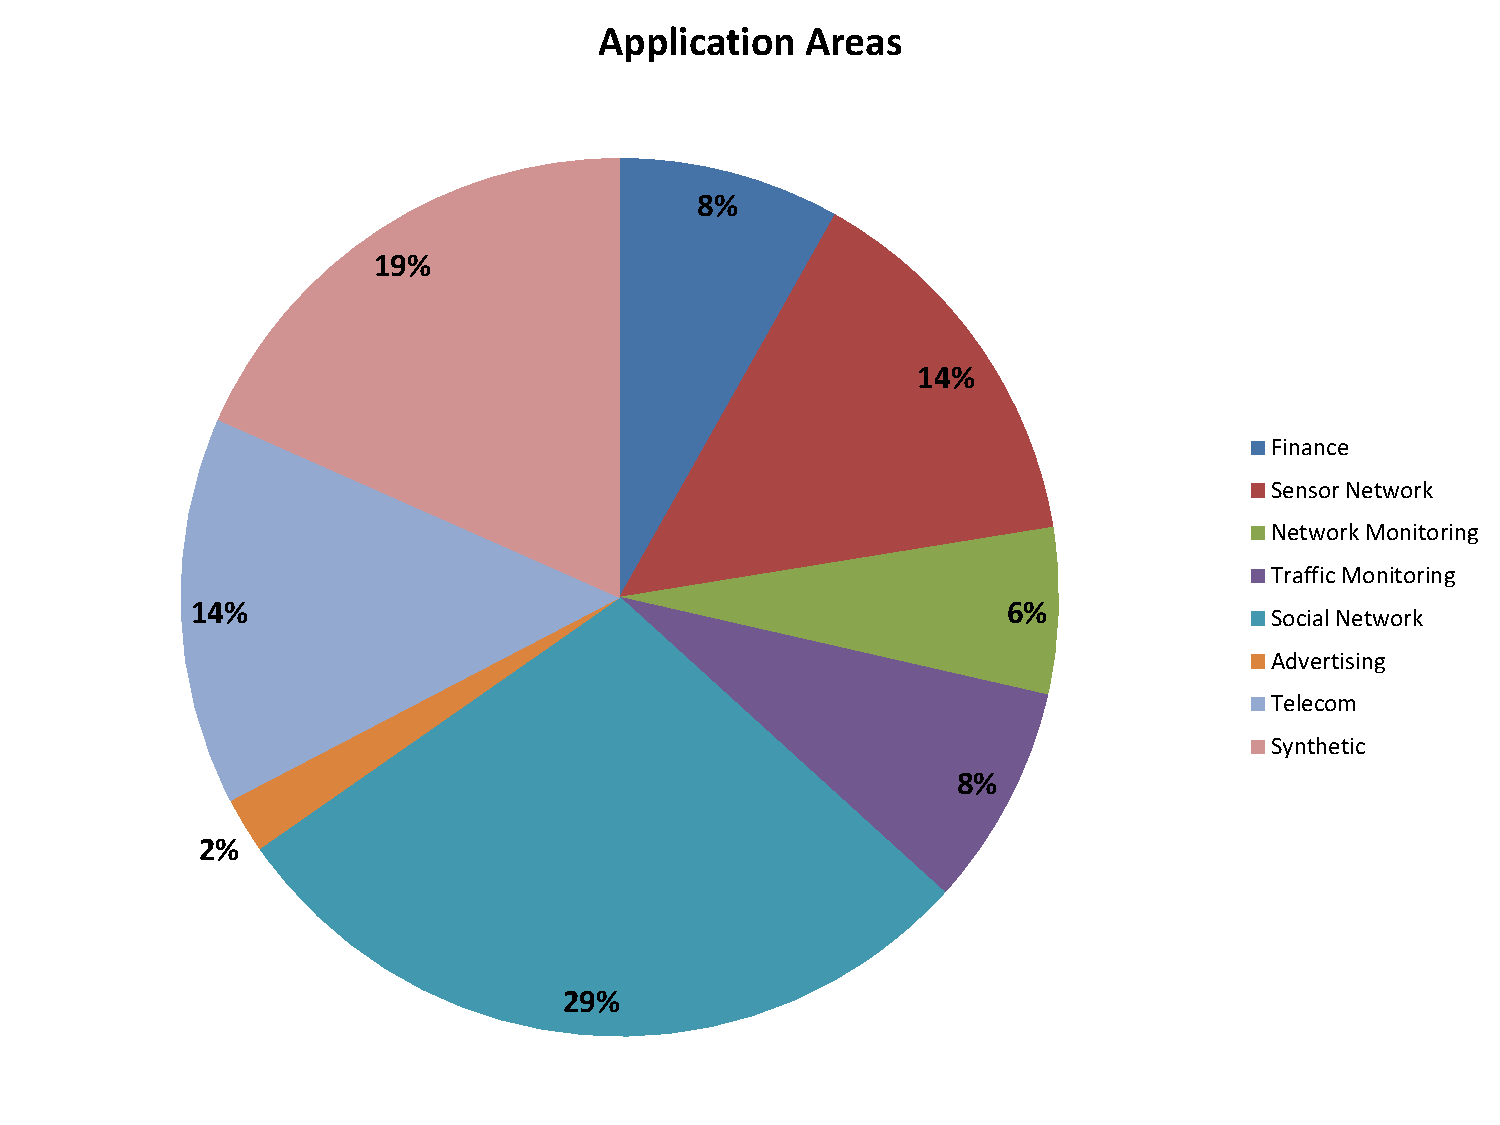
\includegraphics[width=0.8\textwidth]{images/ApplicationSelection.pdf}
	\caption{Relevance of application areas in the searched papers.}
	\label{fig:app_selection_areas}
\end{figure}

Figure \ref{fig:app_selection_areas} shows the representation of each application area in the researched papers.



\section{Applications}
\label{sec:applications}

In this section is list all applications that compose the benchmark suite as well as a description of each one of them and a chart displaying the data flow of the application with streams, operators and sinks.

\subsection{Word Count (WC)}

Receives a stream of sentences, splits them into words and count the number of occurrences of each word using an associative array (Figure \ref{fig:app_wordcount}). Based on the value of the word the tuple is sent to one instance of the \emph{Word Count} operator, ensuring that the same word goes always to the same instance in order to keep the consistency of the counters. Dayarathna, Takeno and Suzumura \cite{dayarathna2011performance} use a similar application to count hashtags from Twitter.

\begin{figure}[!ht]
	\centering
	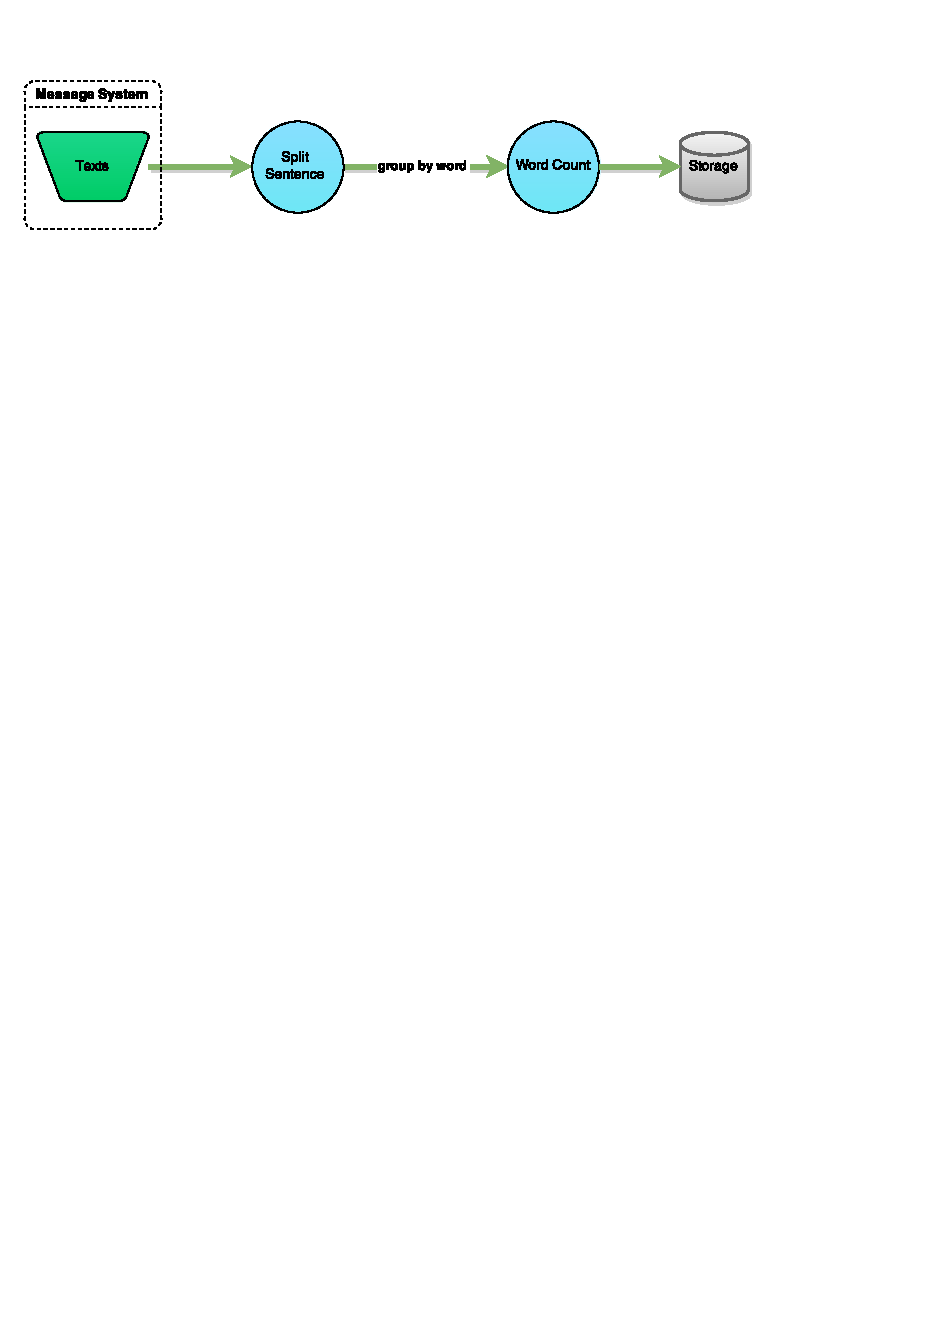
\includegraphics[width=0.8\textwidth]{images/apps/WordCount.pdf}
	\caption{Data flow of the Word Count application}
	\label{fig:app_wordcount}
\end{figure}

\subsection{Log Processing (LP)}

The \emph{Log Processing} application receives as input logs of HTTP web servers. These logs are usually in the \emph{Common Log Format} and need to be parsed in order to extract the relevant data fields, such as the \emph{timestamp}, \emph{request verb}, \emph{resource name}, \emph{IP address} of the user and \emph{status code}.

With the events parsed, the stream is duplicated to three operators. The \emph{Volume Count} operator counts the number of visits per minute, with each event received representing a single visit. The \emph{Status Counter} operator stores the number of occurrences of each \emph{status code} in an associative array. And the \emph{Geography} operator get the location of the user using its IP address by using an IP location database, such as the MaxMind GeoIP, and emits a new event with the name of the country and city of the user, if found.

The subsequent operator, \emph{GeoStats}, receives the location information and updates the counter per country and city, emitting the new values.

\begin{figure}[!ht]
	\centering
	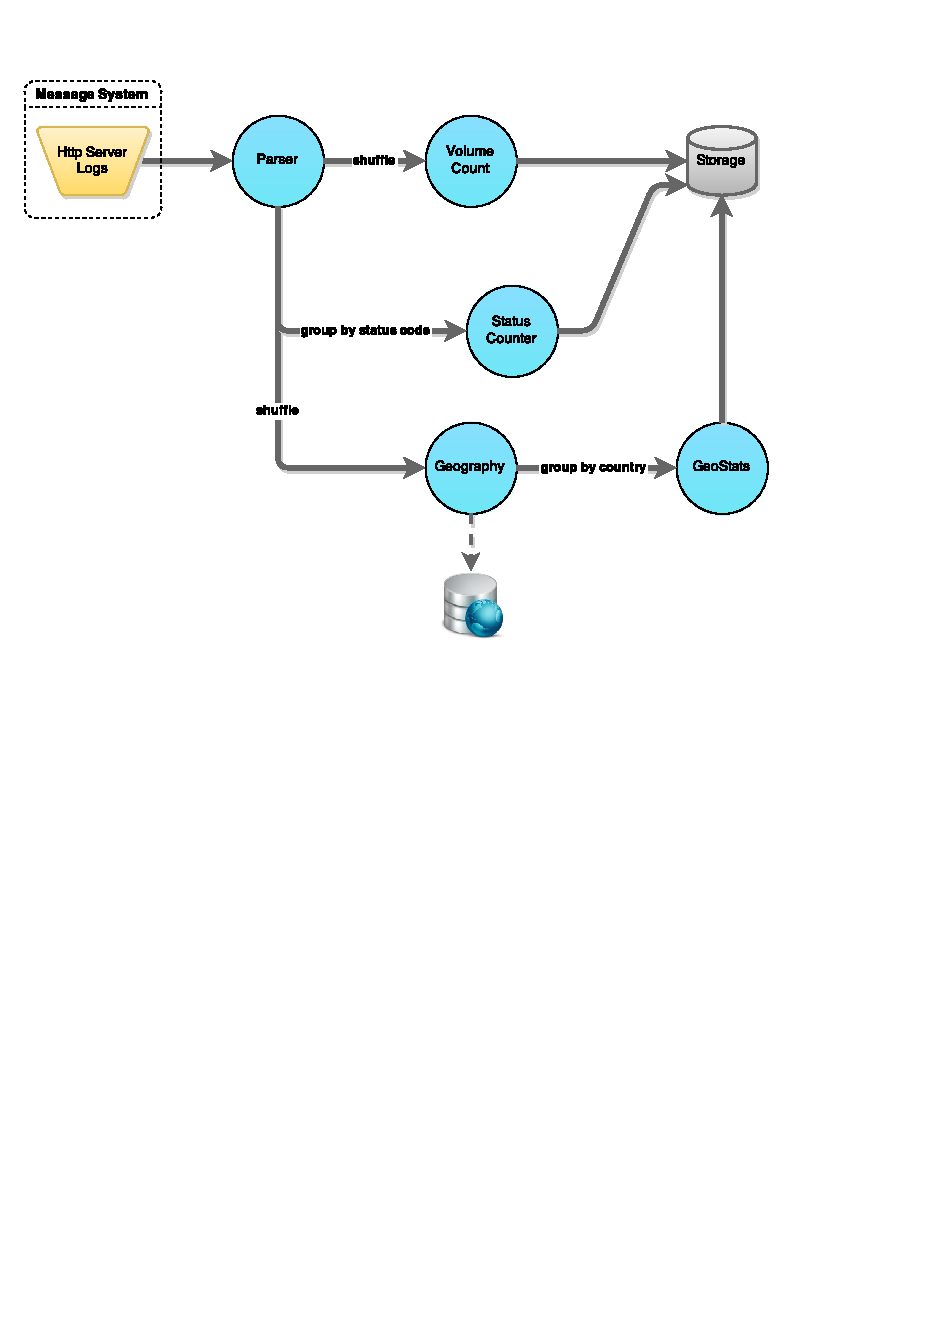
\includegraphics[width=0.8\textwidth]{images/apps/LogProcessing.pdf}
	\caption{Data flow of the Log Processing application}
	\label{fig:app_log_processing}
\end{figure}

\subsection{Traffic Monitoring (TM)}

The \emph{Traffic Monitoring} application receives events in real-time emitted from vehicles, containing its IDentification, location (latitude and longitude from a GPS), direction, current speed, and timestamp.

\begin{figure}[!ht]
	\centering
	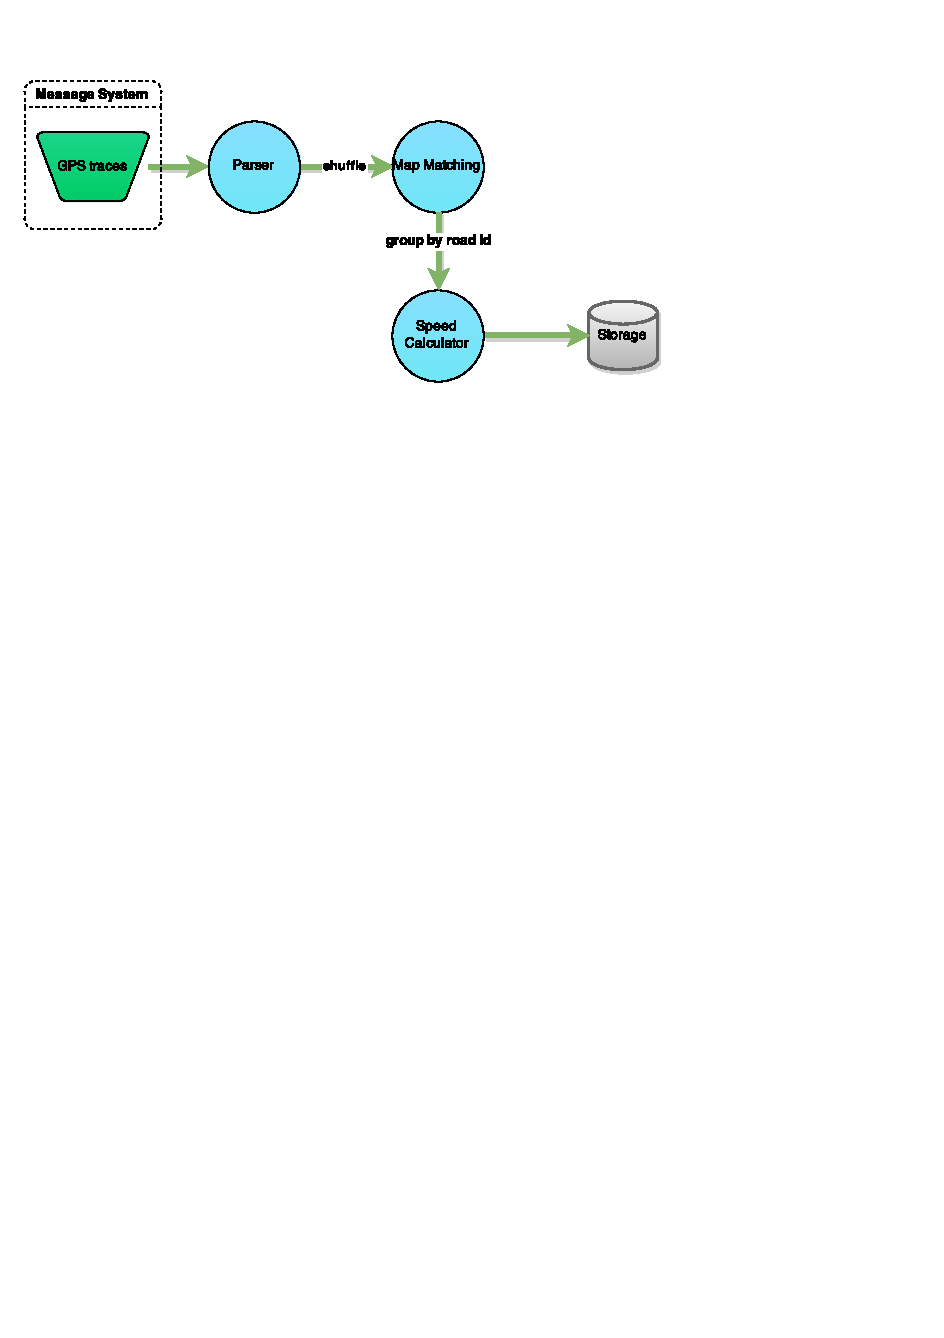
\includegraphics[width=0.8\textwidth]{images/apps/TrafficMonitoring.pdf}
	\caption{Data flow of the Traffic Monitoring application}
	\label{fig:app_traffic_monitoring}
\end{figure}

The \emph{Map Matching} operator is responsible for receiving these events and identifying the road that vehicle is riding. To do so, this operator is initialized with a \emph{bounding box} that corresponds to the borders of the city being monitored, enabling the component to eliminate the events that occurred outside of the city limits. It also loads at initialization a \emph{shapefile} with all roads of the city, and with that it can lookup the road that the vehicle is is by using its current location.

After finding the road, the component appends the road ID to the event and forwards it to the \emph{Speed Calculator} operator. This component calculates the average speed of the vehicles for each road, creating a new event with the timestamp, ID of the road, average speed and number of vehicles on the road.


\subsection{Machine Outlier (MO)}

Receives resource usage readings from computer in a network, calculates the Euclidean distance of a reading from the cluster center of a set of readings in a given time period and applies the BFPRT algorithm to detect abnormal readings \cite{yoon2007approach}.

\begin{figure}[!ht]
	\centering
	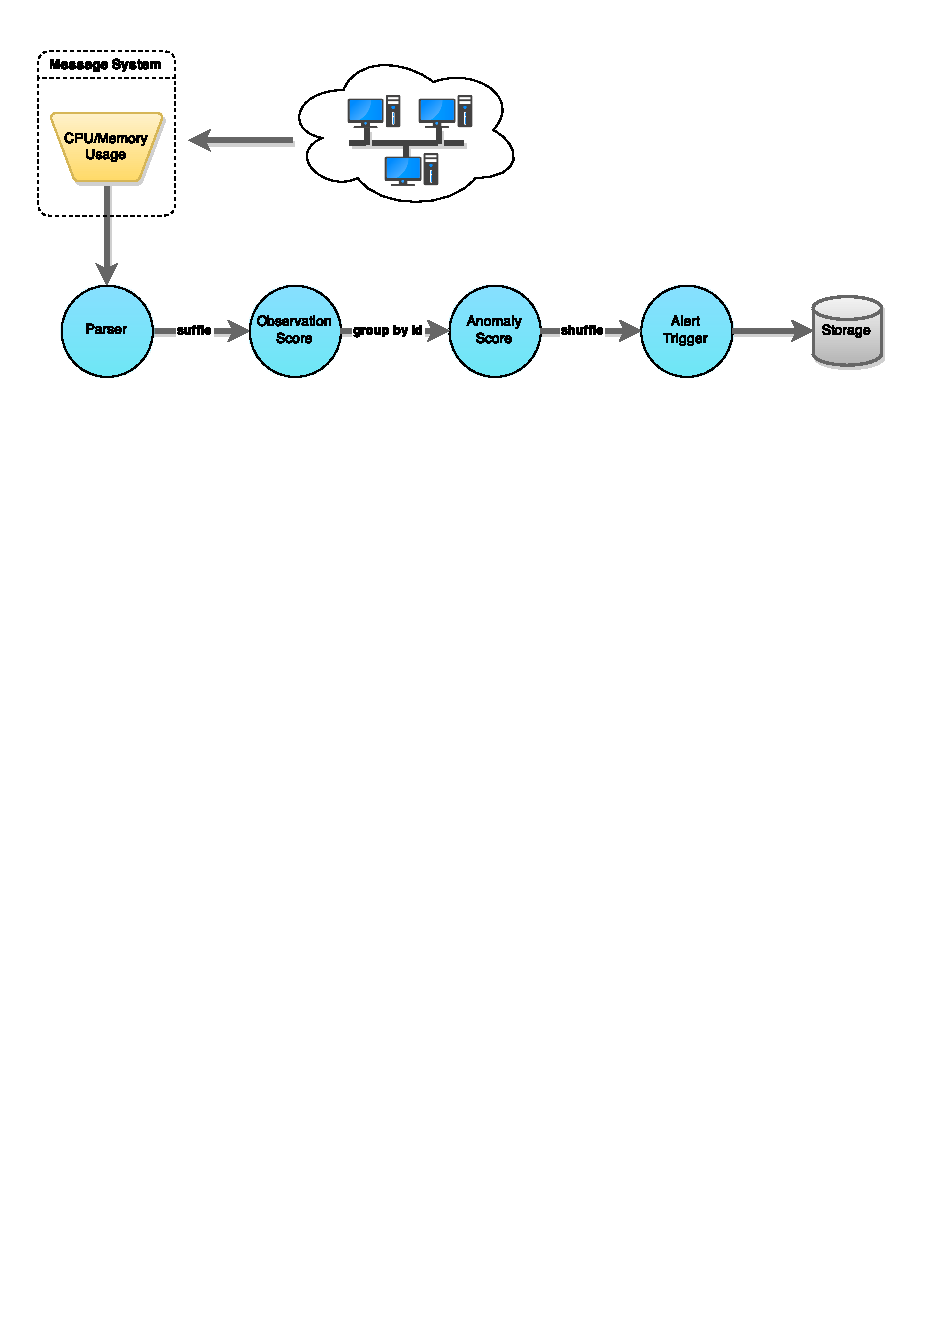
\includegraphics[width=0.8\textwidth]{images/apps/MachineOutlier.pdf}
	\caption{Data flow of the Machine Outlier application}
	\label{fig:app_machine_outlier}
\end{figure}

\subsection{Sentiment Analysis (SA)}

The \emph{Sentiment Analysis} application uses a simple NLP technique for calculating the sentiment of sentences, consisting of counting positive and negative words and using the difference to indicate the polarity of the sentence.

The application receives a stream of \emph{tweets} in the JSON format, each \emph{tweet} corresponds to an event that has to be parsed in order to extract the relevant fields, in this case the \emph{ID} of the tweet, the \emph{language} and the \emph{message}.

\begin{figure}[!ht]
	\centering
	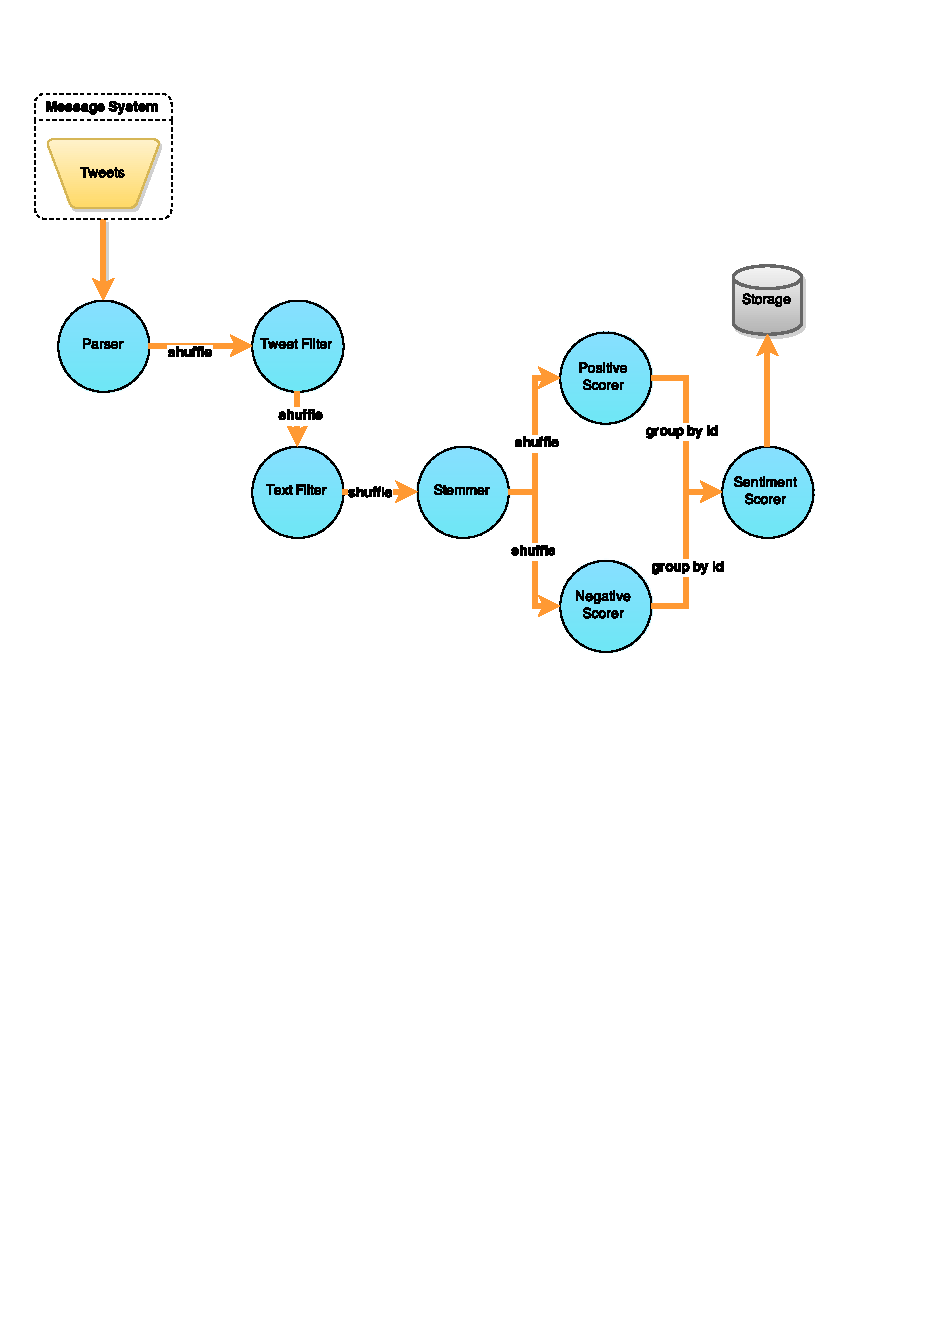
\includegraphics[width=0.8\textwidth]{images/apps/TwitterSentiment2.pdf}
	\caption{Data flow of the Sentiment Analysis application}
	\label{fig:app_sentiment_analysis}
\end{figure}

After being parsed, the tweets are filtered, removing those that have been written in a language that is not supported by the application. By default only the English language is supported, to extend the support the operators that load the negative/positive list of words would have to switch lists between languages for each new event.

Next, the tweets go through the \emph{Stemmer}, which removes \emph{stop words} from the message, which are words that usually don't carry sentiment, and thus are irrelevant for the next steps in the application.

With the tweets filtered and cleaned, the stream is duplicated to two operators that will count the number of occurrences of positive and negative words. Using the ID of the tweet these two streams will be joined, creating a new event with both the positive and the negative counters. The next operator will then calculate sentiment of the tweet, which will be positive if the number of occurrences of positive words is greater than the negative ones, or negative otherwise.

% need to create new data flow

\subsection{Spam Filter (SF)}

The \emph{Spam Filter} application uses Naive Bayes \cite{androutsopoulos2000evaluation} to analyse if email messages are spam (or ham). As opposed to other applications that required an offline training phase, in this case there is a training stream that enables the application to be trained in real-time. In a performance test however, the training and analysis should be evaluated separately.

Alternatively, the application also supports offline training, which means that the probabilities of words are pre-loaded in the \emph{Word Probability} operator. In this case the events emitted by the \emph{Tokenizer} don't need to be grouped by \emph{word}, but shuffled since all instances of the \emph{Word Probability} operator will have the probabilities of all words.

The advantage of this approach is that the recovery of an operator after a failure is very quick since it only needs to load the file containing the probabilities, instead of having the be trained again. The only downside is that instances of this operator will consume more memory since they will load the probabilities for all words.

\begin{figure}[!ht]
	\centering
	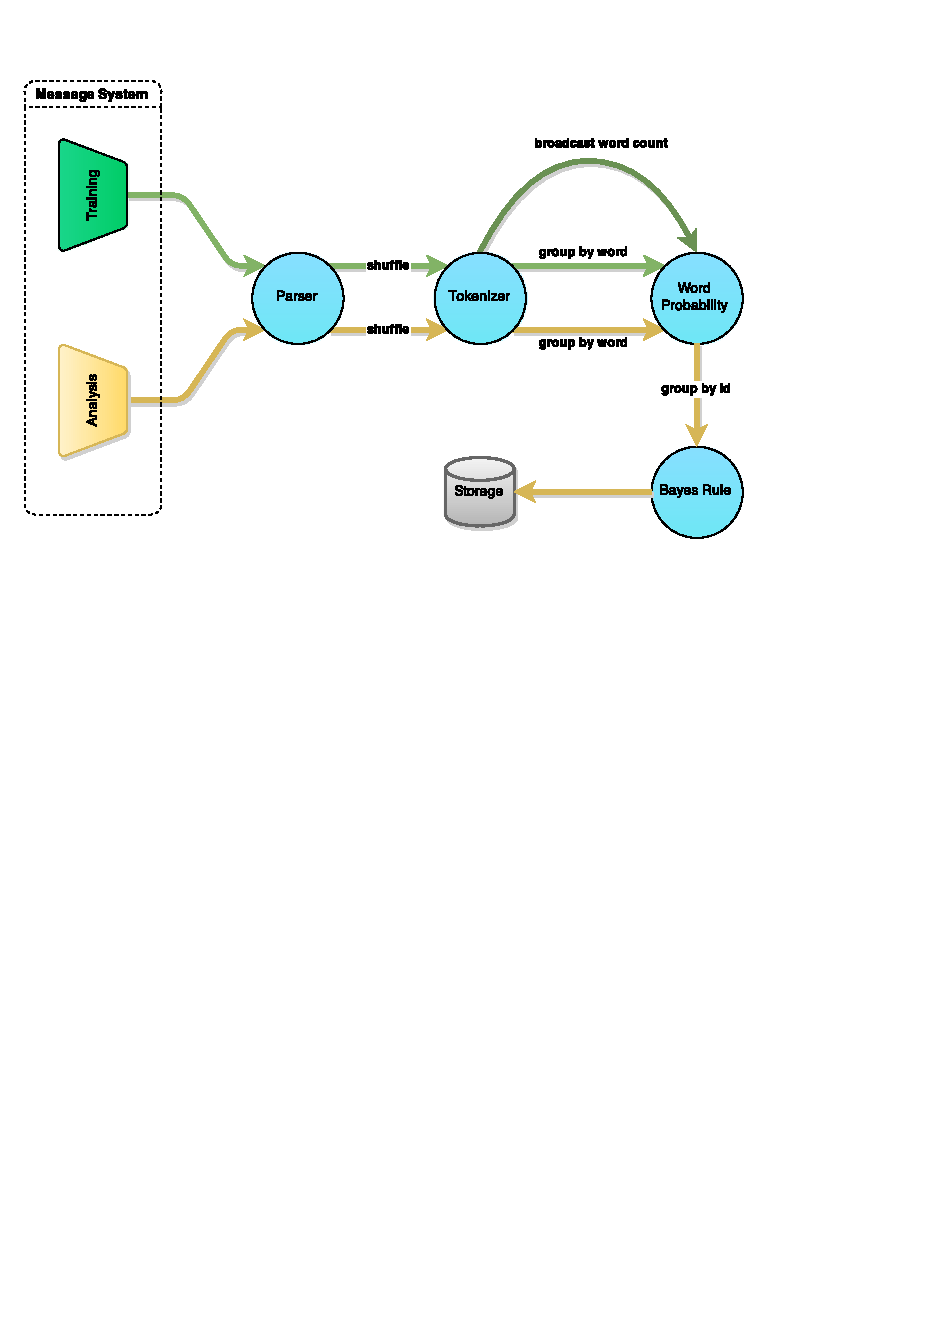
\includegraphics[width=0.8\textwidth]{images/apps/SpamFilter.pdf}
	\caption{Data flow of the Spam Filter application}
	\label{fig:app_spam_filter}
\end{figure}

\subsection{Trending Topics (TT)}

Extracts topics from a stream of \textit{tweets}, count the occurrences for each topic in a window of events (limited size) and emits only the popular topics (i.e. the trending topics).

The occurrences of topics is tracked by a sliding window which is advanced in a fixed interval of time. The use of a sliding window reduces the memory usage since only recent events are stored, it also makes since because the application is interested in detecting only new trends. To increase scalability an \emph{Intermediate Ranking} operator is used to rank a subset of topics, and in a fixed interval of time these intermediate rankings are sent to the \emph{Total Ranking} operator, which will merge the intermediate rankings and emit the final ranking of topics, i.e. the trending topics.

An example of such application is the TwitterMonitor \cite{mathioudakis2010twittermonitor}, a system that detects trends in real-time from Twitter. This application is also used to compare the performance of a traffic monitoring and analysis tool called BlockMon \cite{simoncelli2013scaling} with Storm and Apache S4.

\begin{figure}[!ht]
	\centering
	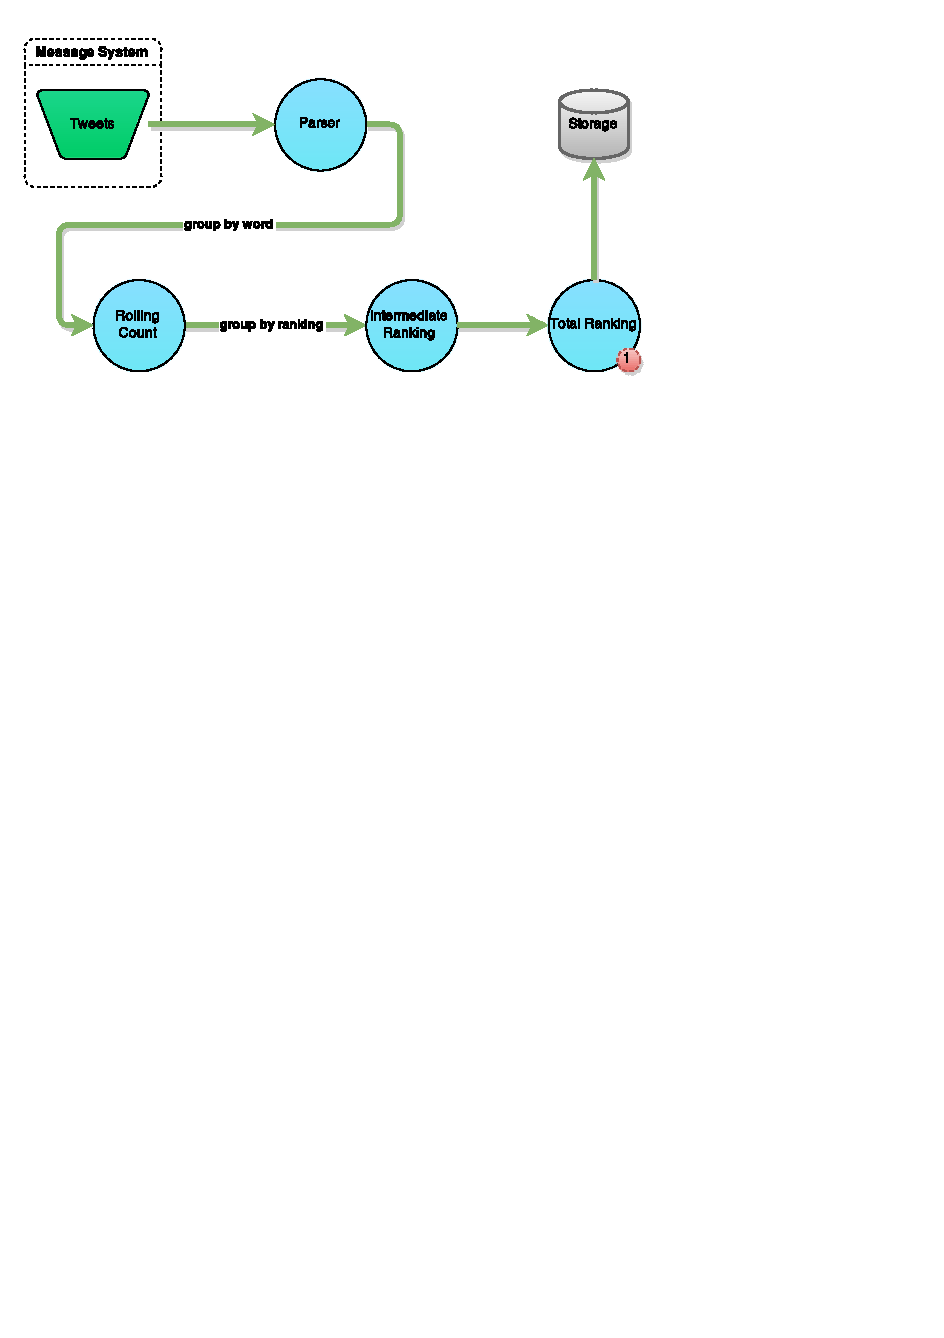
\includegraphics[width=0.8\textwidth]{images/apps/TrendingTopics.pdf}
	\caption{Data flow of the Trending Topics application}
	\label{fig:app_trending_topics}
\end{figure}

\subsection{Click Analytics (CA)}

Receives a clickstream from users accessing a website as input. These input events are logs from the web server, usually in the \emph{Common Log Format}, which means they have to be parsed in order to extract the relevant data fields. The most common fields are the \emph{timestamp}, \emph{URL}, \emph{IP address} of the user, ID of the user (the IP address is used if the ID is not available).

After the \emph{Parser} operator the stream is splitted into two, with events being replicated to both of them. In the \emph{RepeatVisit} operator, events are grouped based on the URL and ID of the user because these two fields are used as key in an associative array to verify if the user has already visited the URL or not. The downstream operator, \emph{VisitStats} then counts the total number of visits and the unique visits (first time user visits an URL).

On the other stream events are randomly distributed among the instances of the \emph{Geography} operator. This operator, on initialization, creates a connection to a database IP locations, such as the MaxMind GeoIP database. Upon receiving an event, the operator query the database with the user IP address and receives as a result the location of the user. The operator then extracts from the location the name of the city and country and forwards it as a new event to the \emph{GeoStats} operator.

The \emph{GeoStats} operator stores one object for each country in an associative array, this object has a counter of visits per country and an associative array with counters per city. After each event the operator updates the counters for the country and city and emits the new values.

\begin{figure}[!ht]
	\centering
	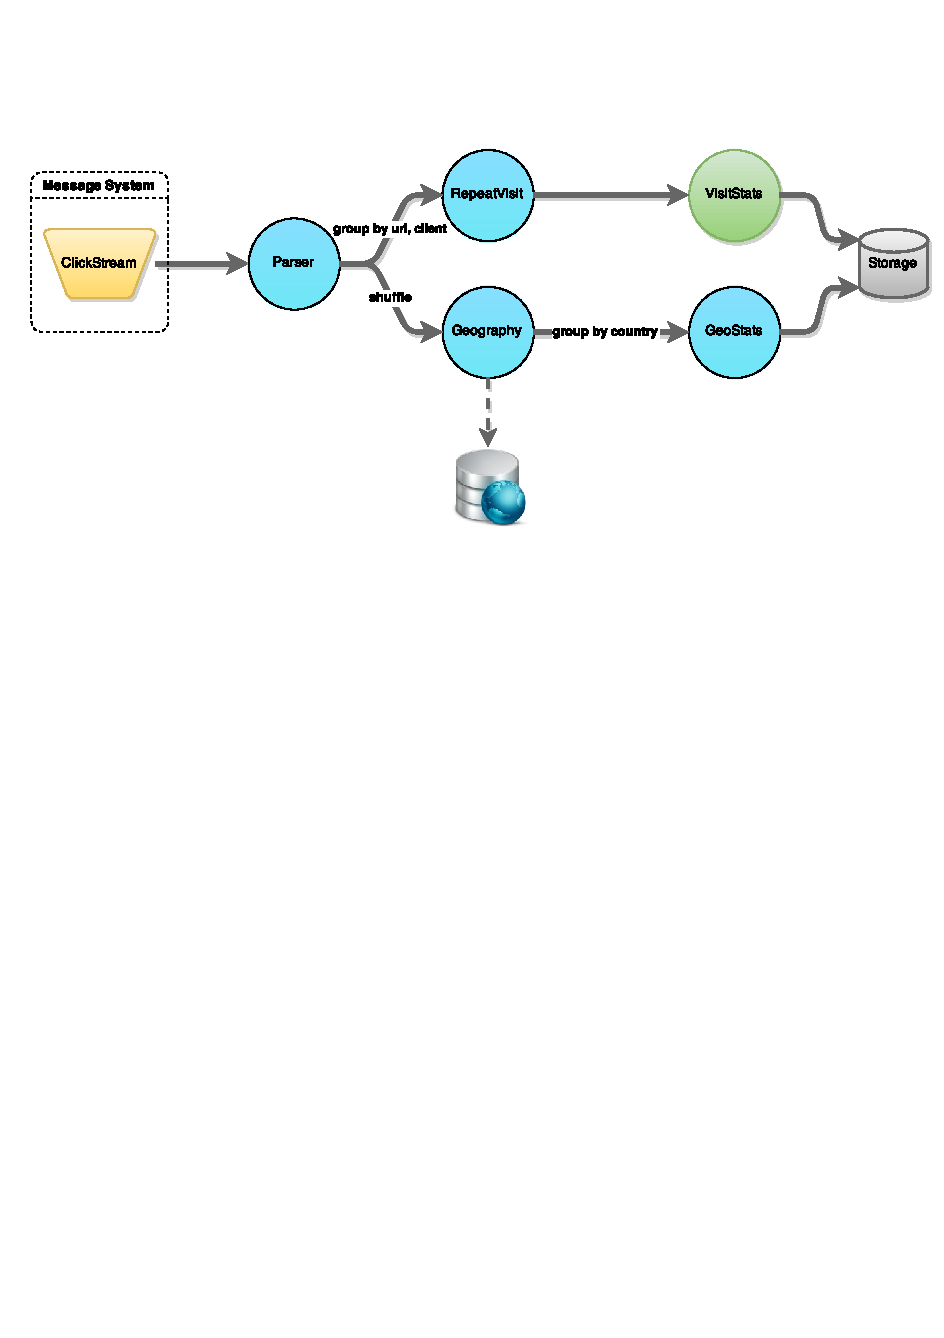
\includegraphics[width=0.8\textwidth]{images/apps/ClickAnalytics.pdf}
	\caption{Data flow of the Click Analytics application}
	\label{fig:app_click_analytics}
\end{figure}

\subsection{Fraud Detection (FD)}

Uses a Markov model \cite{srivastava2008credit}, created in an offline phase, to calculate the probability of a credit card transaction being a fraud.

\begin{figure}[!ht]
	\centering
	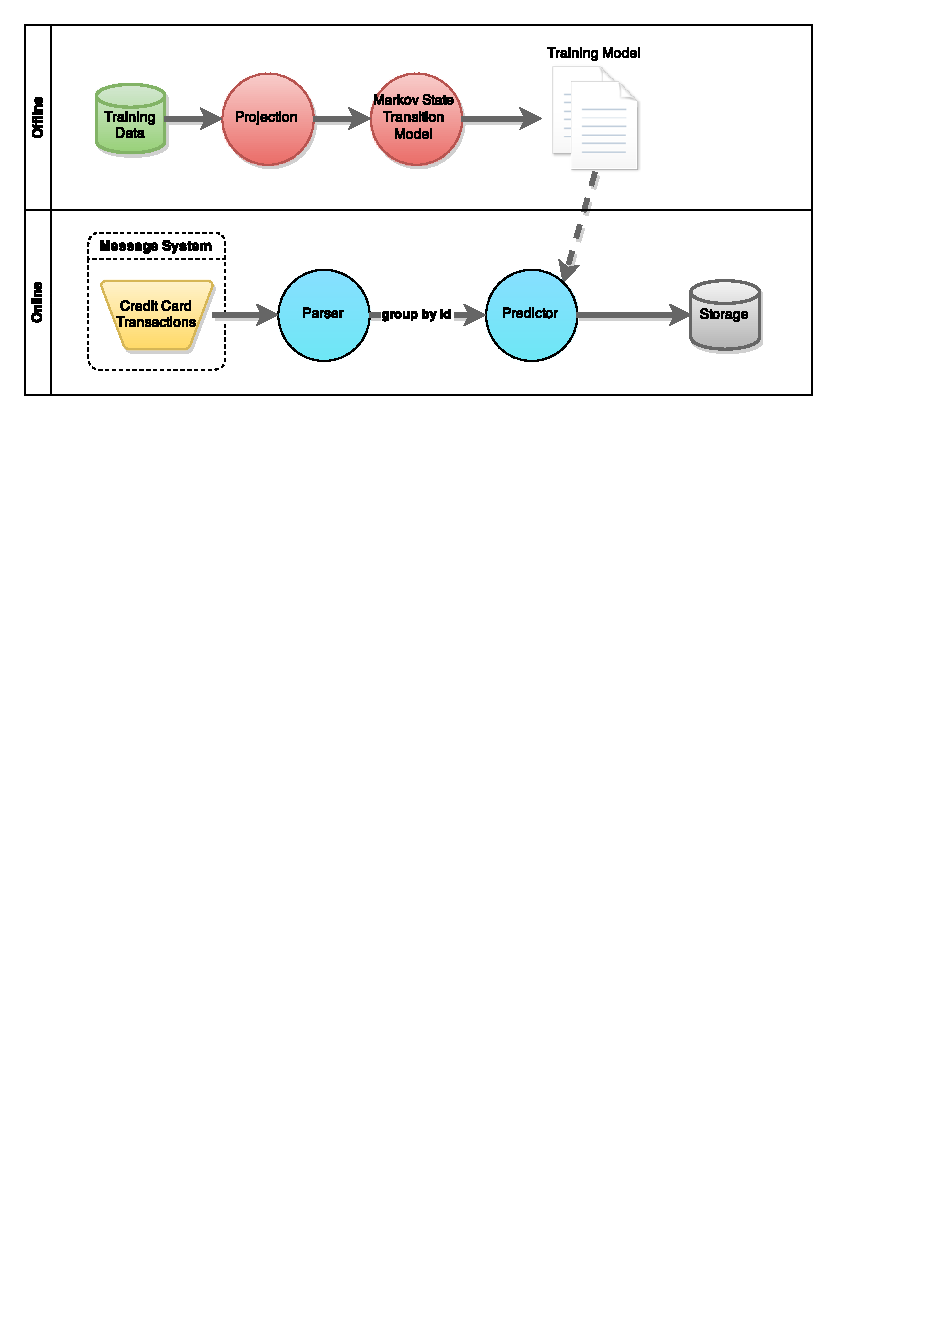
\includegraphics[width=0.8\textwidth]{images/apps/FraudDetection.pdf}
	\caption{Data flow of the Fraud Detection application}
	\label{fig:app_fraud_detection}
\end{figure}

\subsection{Spike Detection (SD)}

The \emph{Spike Detection} application receives a stream of readings from sensors in order to monitor spikes in their values. The \emph{Moving Average} operator receives these events grouped by the ID of the device since it is going to store the last $N$ values received for each device, with $N$ being the size of the window. When a new event is received, the operator adds the new value to the list of values of the device and emits a new event with the ID of the device, the current value ($V_{curr}$) and the moving average ($V_{avg}$) of values.

The operator downstream (\emph{Spike Detection}) receives these events randomly and based on a threshold ($t$) value specified at initialization it checks if the current event is a spike or not, using Formula \ref{eq:spike_detect}.

\begin{equation}\label{eq:spike_detect}
    isSpike=
    \begin{cases}
      true, & \text{if}\ abs( V_{curr} - V_{avg} ) > t \times V_{avg} \\
      false, & \text{otherwise}
    \end{cases}
\end{equation}

\begin{figure}[!ht]
	\centering
	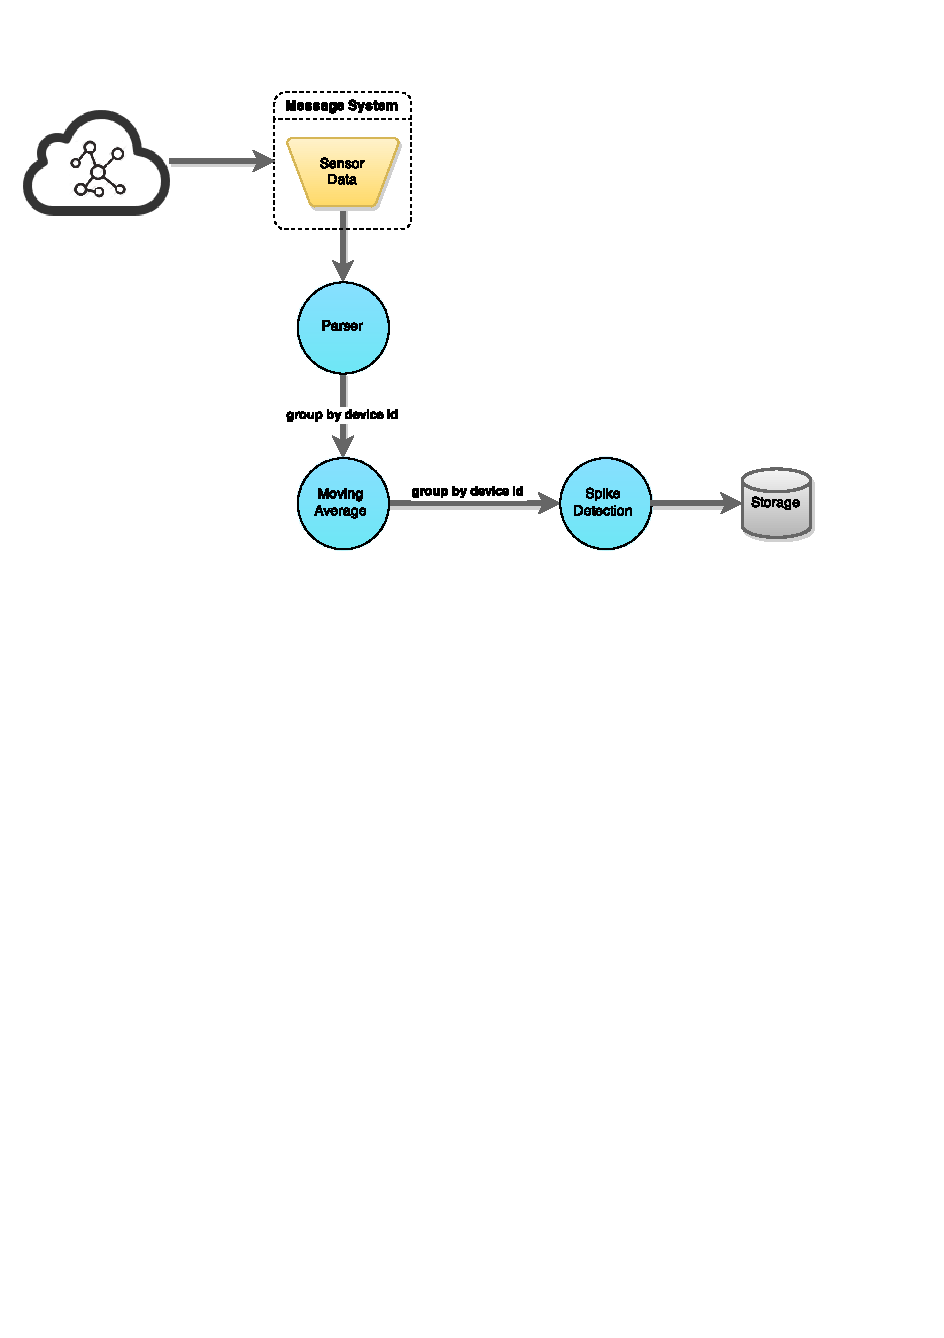
\includegraphics[width=0.8\textwidth]{images/apps/SpikeDetection.pdf}
	\caption{Data flow of the Spike Detection application}
	\label{fig:app_spike_detection}
\end{figure}

\subsection{Bargain Index (BI)}

An application that seeks stocks that are for sell in quantity and with prices below the mean observed in recent operations. The application calculates the bargain index, a scalar value that represents the magnitude of the bargain \cite{gedik2008spade, andrade2009scale, dayarathna2013automatic}.


\begin{figure}[!ht]
	\centering
	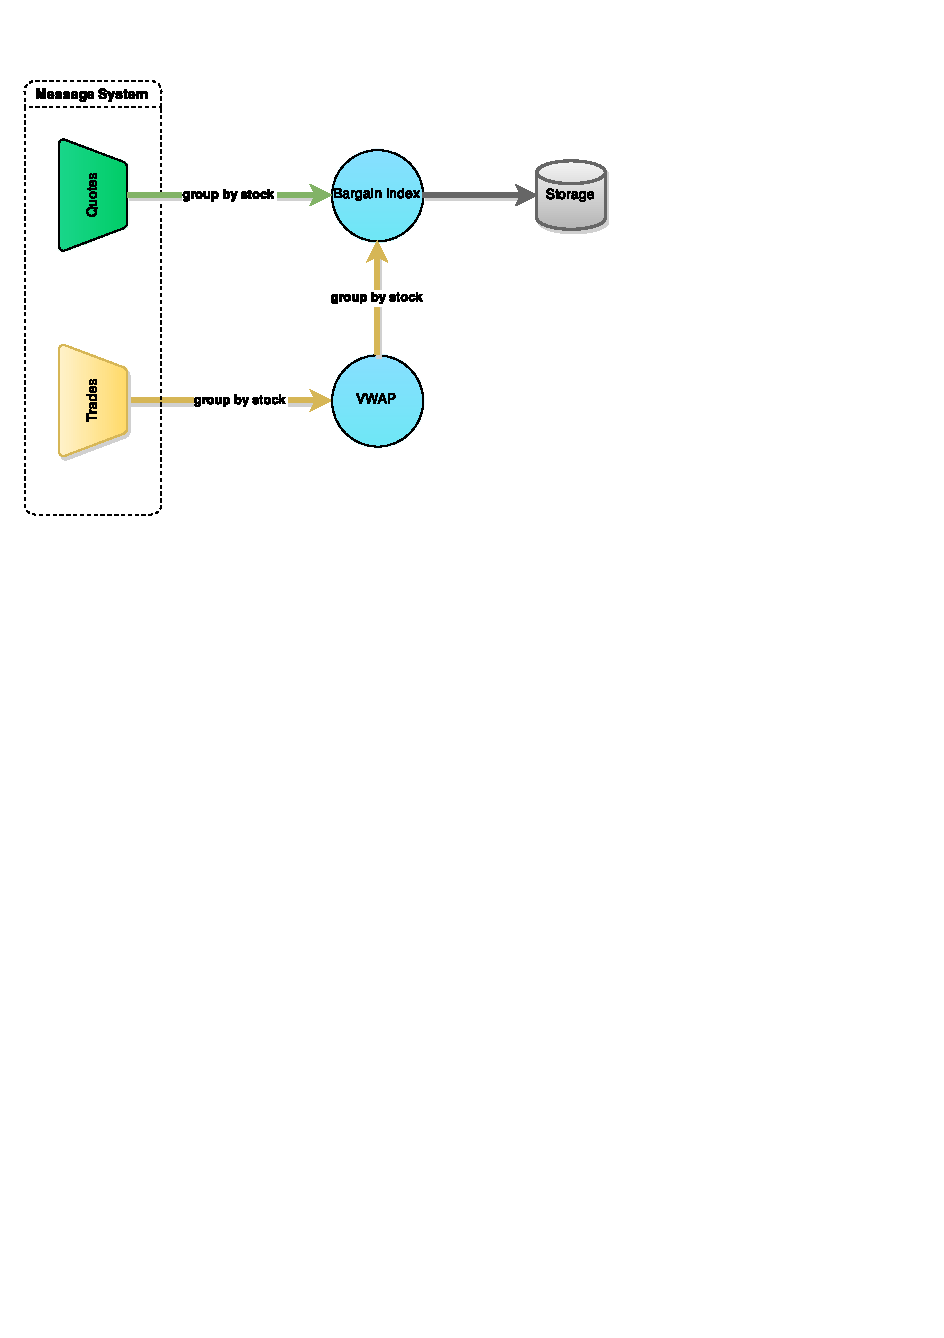
\includegraphics[width=0.8\textwidth]{images/apps/BargainIndex.pdf}
	\caption{Data flow of the Bargain Index application}
	\label{fig:app_bargain_index}
\end{figure}

The dataflow of the bargain index application, seen in Figure \ref{fig:app_bargain_index}, receives as input TAQ (Trade and Quote) records, where a \emph{trade} is a transaction that already occurred and it is characterized by the price of the stock and the amount that was sold/bought. Whereas a \emph{quote} transaction can be a \emph{bid} or an \emph{ask}, the first being issued by someone who is looking to buy stocks and the second by someone trying to sell them. The \emph{source} component receives both types of transactions and splits them into two different data streams.

With the stream of trading transactions the first component calculates the product of $P$ (price) and $V$ (volume). The second component does the summation of a sliding window of 15 tuples ($\sum_{i=1}^{W_{size}}P_{i}V_{i}$), with $Advance = 1$. The next component calculates the Volume-Weighted Average Price (VWAP), one of the main metrics for evaluating the performance of a trade \cite{di2010applications, kim2010electronic}, as follows

\begin{equation}
P^{VWAP} = \frac{\sum_{i=1}^{N}P_{i}V_{i}}{\sum_{i=1}^{N}V_{i}}
\end{equation}\cite{kakade2004competitive}, where $P_{i}$ and $V_{i}$ are the price and trading volume, respectively, of a transaction $i = (1,2,...,N)$.

When the VWAP stream joins the quotes stream, the component can analyze each stock offer to judge if the trade is good or not. If the ask price is lower than the VWAP price, then it is a good trade. The question is how good is this stock offer? This question can be answered with the bargain index, defined as
%\exp(P^{VWAP} - P_{ask}) \times V_{ask}
\begin{equation}
bargainIndex = 
\begin{cases}
  \exp(P^{VWAP} - P_{ask}) \times V_{ask}, & \text{if}\ P^{VWAP} > P_{ask} \\
  0, & \text{otherwise}
\end{cases}
\end{equation} \cite{ranganathan2011constructing}, where $P_{ask}$ is the price of each stock offered and $V_{ask}$ is the amount of stocks available for trade. The the last component can, besides dropping zero indexes (which can be eliminated in the previous component to save network), place orders to buy stocks if the bargain index is above a certain threshold.

\subsection{Reinforcement Learner (RL)}

%Concepts at \cite{strehl2008analysis}.

An example of such application is in the paper the introduces the S4 system \cite{neumeyer2010s4}, which uses an application that consumes events coming from a search advertising system, measures its performance under the current parameters and applies an adaptation algorithm to determine new parameters for improving the advertising performance.

\begin{figure}[!ht]
	\centering
	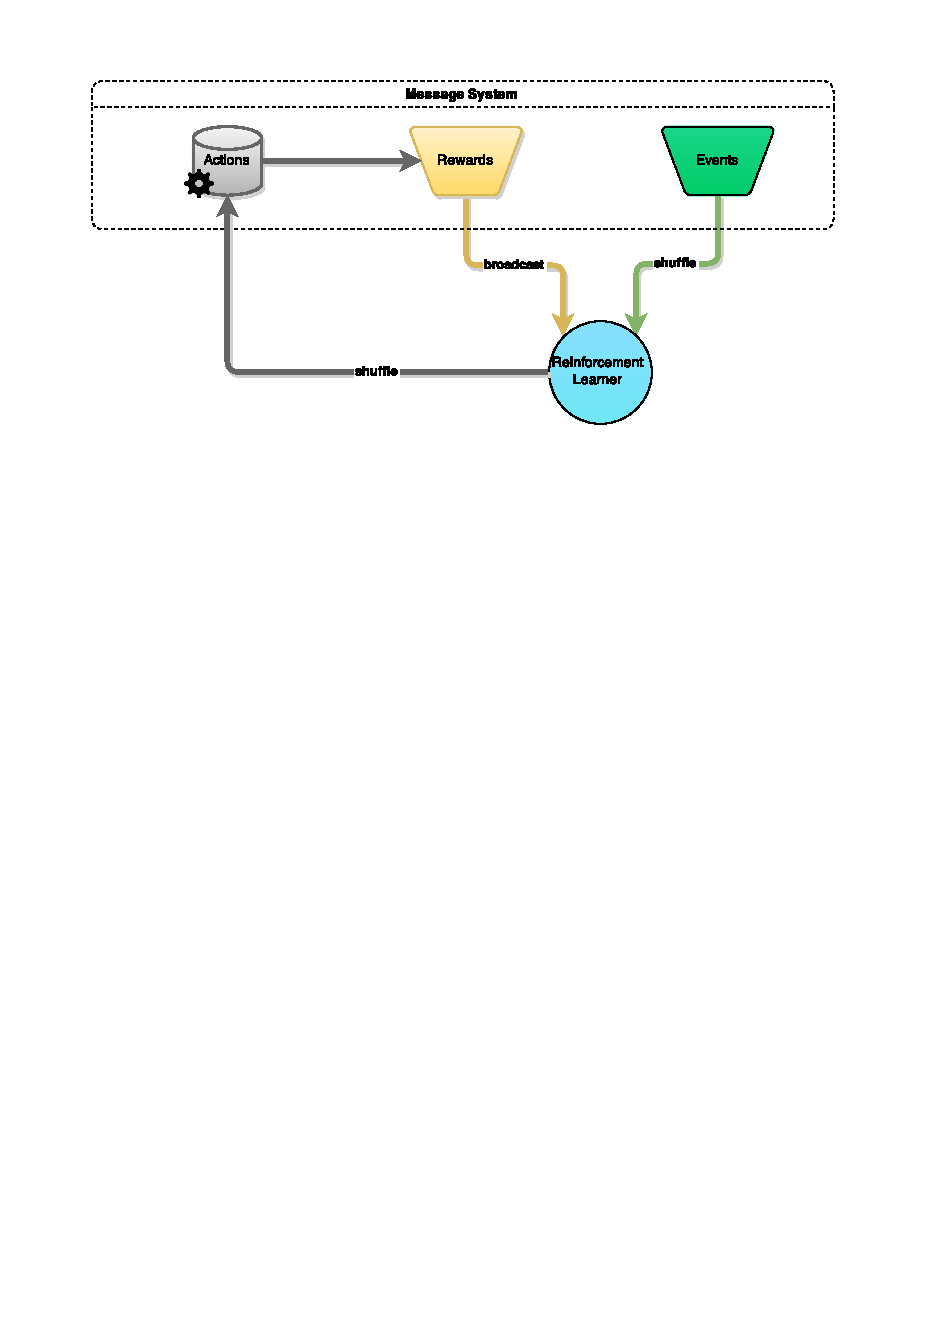
\includegraphics[width=0.8\textwidth]{images/apps/ReinforcementLearner.pdf}
	\caption{Data flow of the Reinforcement Learner application.}
	\label{fig:app_reinforcement_learner}
\end{figure}

The \textit{reinforcement learner} operator uses the interval estimate \cite{strehl2008analysis} algorithm and to choose the action to take it uses second order statistics of the reward distribution.

The algorithm can be characterized by two phases: exploration and exploitation. In the beginning the reward distribution does not have enough data, so the the algorithm will choose actions randomly. When enough data is available, the exploitation phase begins, with the algorithm choosing actions with the highest mean reward.

\subsection{Smart Grid Monitoring (SM)}

Monitoring of energy consumption for load prediction and outlier detection. The application was proposed in the DEBS 2014 Grand Challenge\footnote{http://www.cse.iitb.ac.in/debs2014/?page\_id=42}.

\begin{figure}[H]
	\centering
	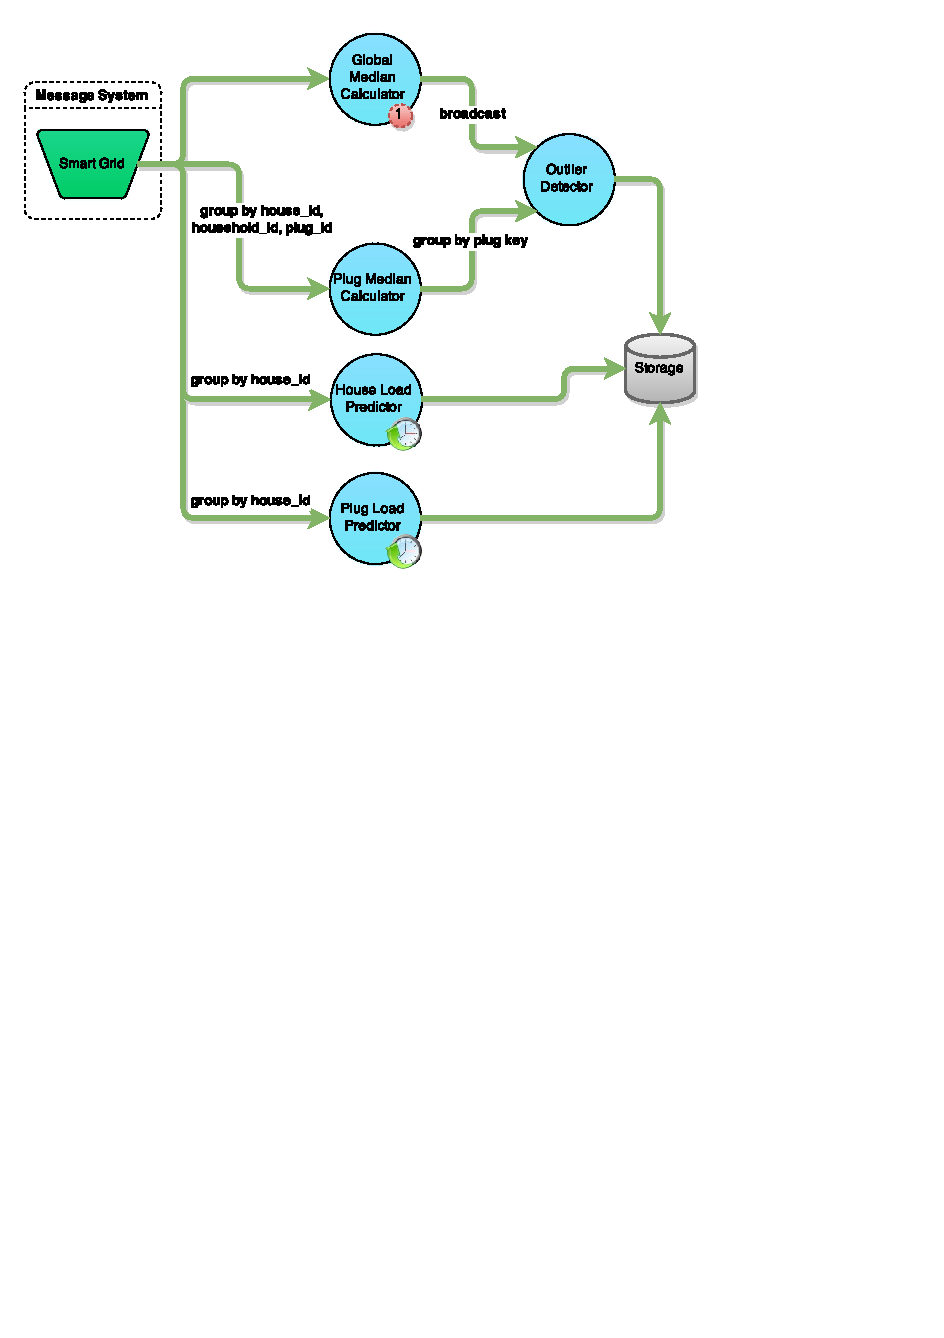
\includegraphics[width=0.8\textwidth]{images/apps/SmartGrid.pdf}
	\caption{Data flow of the Smart Grid Monitoring application.}
	\label{fig:app_smart_grid}
\end{figure}

The application produces two results: outliers per house and house/plug load predictions. The outlier detection is done by first calculating the global median of all houses and then comparing it with the median of each house plug (values above global median are considered outliers). And the prediction uses a the current average and median to predict future loads.

\subsection{Telecom Spam Detection (VS)}

The application (called VoIPSTREAM) detects telemarketing users by analysing call detail records (CDRs) using a set of filters based on time-decaying bloom filters \cite{bianchi2011demand}. This application is used in the evaluation of the BlockMon system \cite{huici2012blockmon}.

\begin{figure}[H]
	\centering
	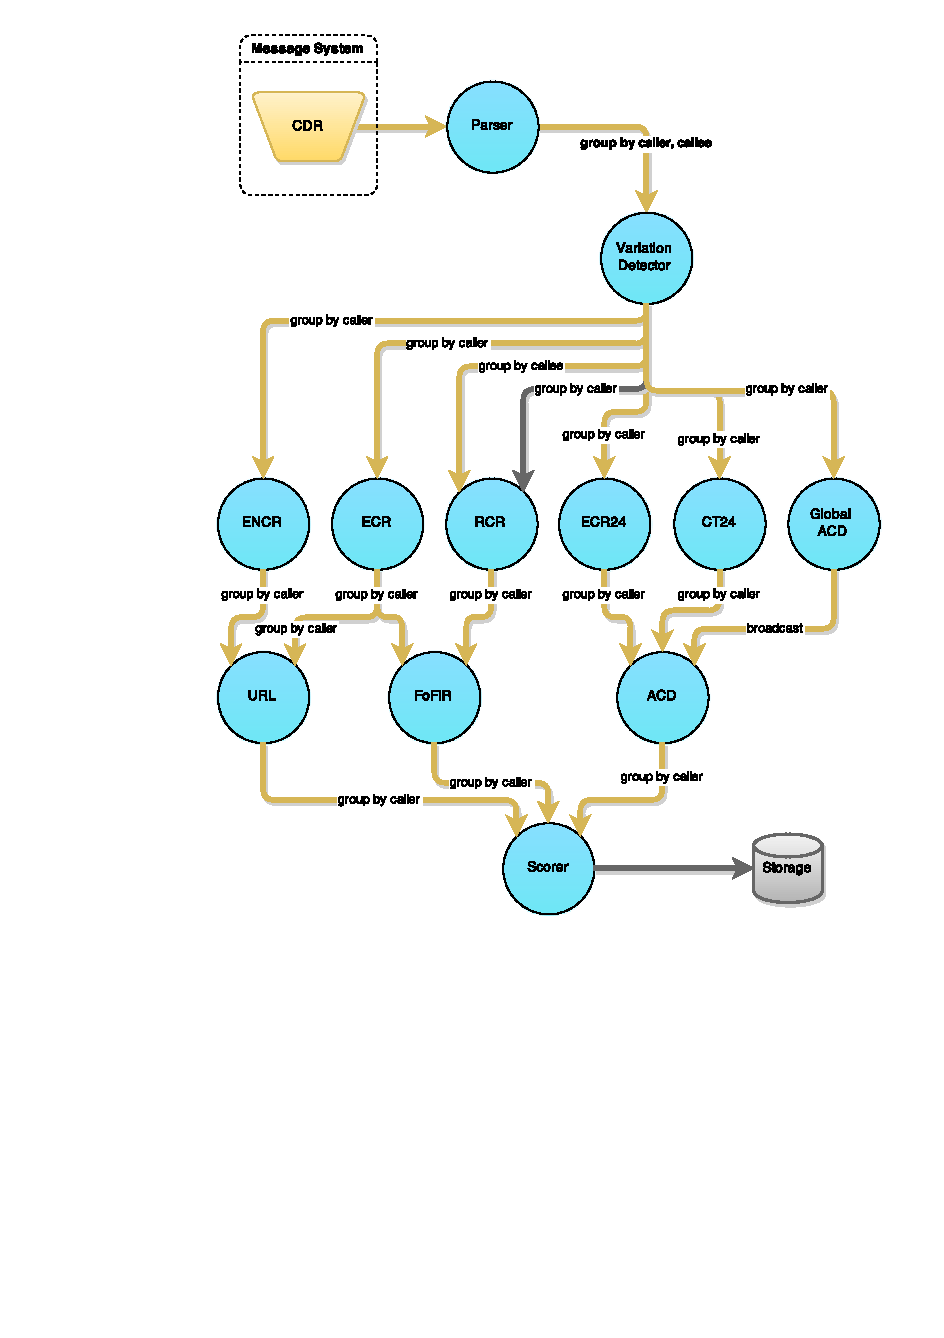
\includegraphics[width=0.8\textwidth]{images/apps/VoIPSTREAM.pdf}
	\caption{Data flow of the VoIPSTREAM application}
	\label{fig:app_voipstream}
\end{figure}


\section{Workload Characterization}
\label{sec:workload-characterization}

To characterize the selected applications, experiments were conducted in a single machine in order to measure the selectivity of operators, the size of the tuples at each operator (using the datasets listed at Section \ref{sec:configuration_datasets}), the memory usage of the applications and the time required to process one tuple per operator.

\begin{figure}[ht!]
    \centering
	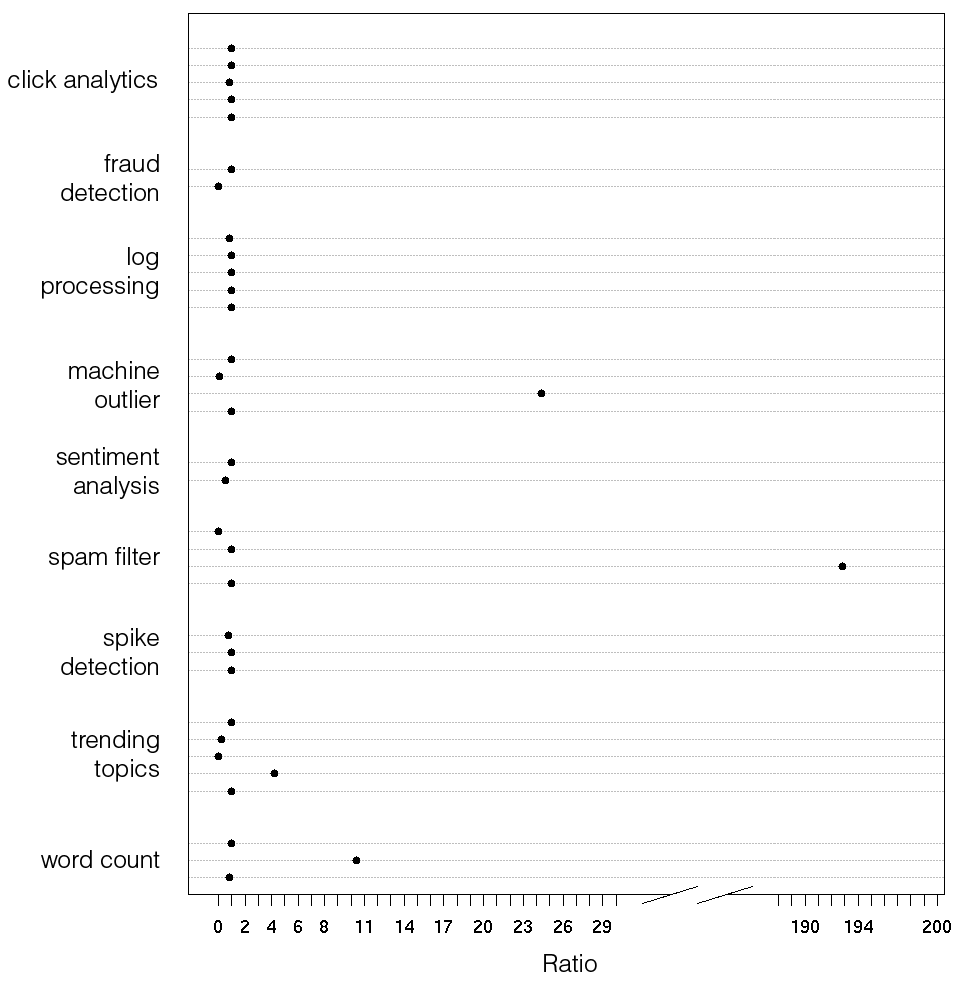
\includegraphics[width=.8\textwidth]{images/selectivity.png}
	\caption{Selectivity of operators}
	\label{fig:operator_selectivity}
\end{figure}

The selectivity (see Figure \ref{fig:operator_selectivity}), as described before, is the ratio between the total number of tuples received and emitted. The greater the selectivity of an operator, the greater will be the number of tuples emitted, but it doesn't necessarily mean that the overhead will also increase, as some ESP systems group tuples together to send them in batches. There are cases where although the selectivity is high, the tuple size is very small as well as the variation.

%TODO increase title of charts
\begin{figure}[ht!]
    \centering
	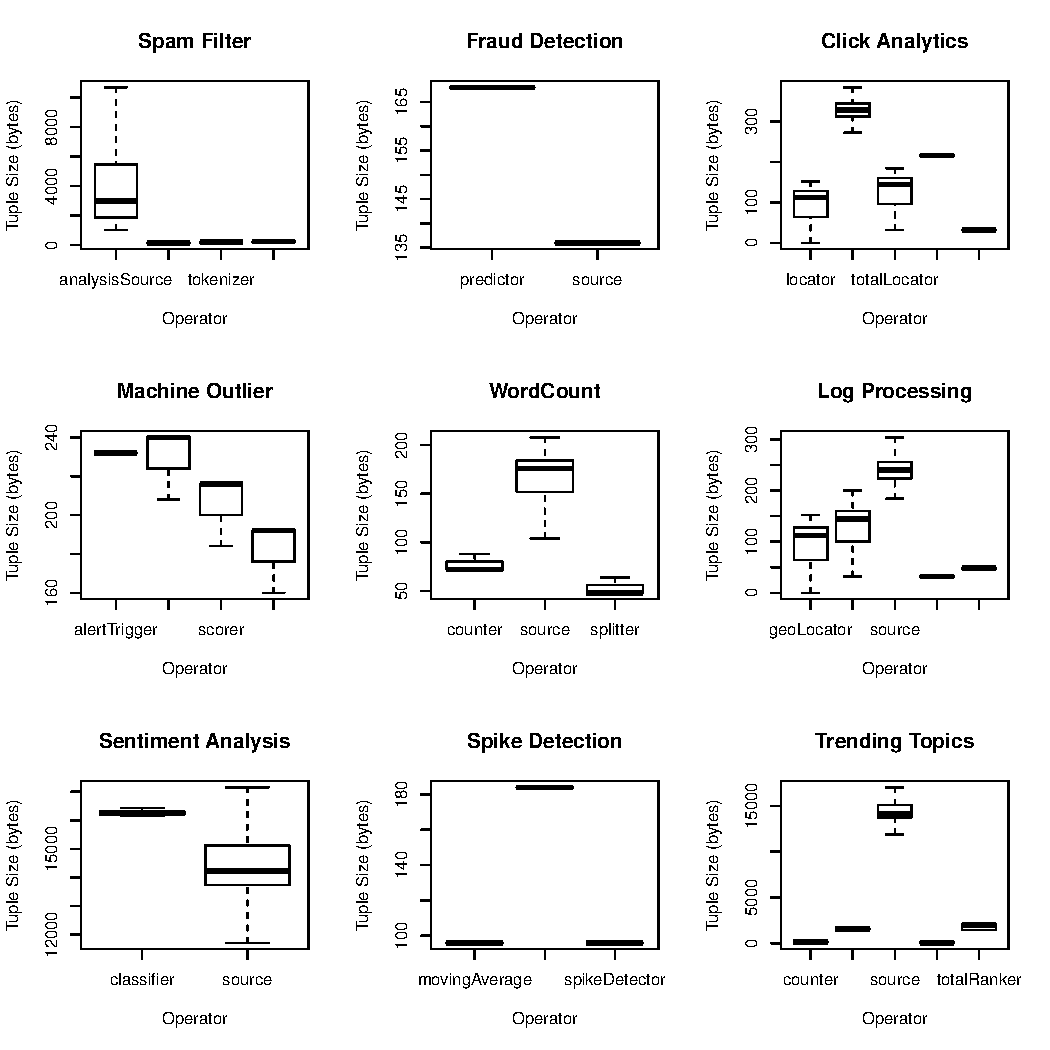
\includegraphics[width=.8\textwidth]{images/tuple_size.pdf}
	\caption{Tuple size per operator}
	\label{fig:tuple_size}
\end{figure}

The usual behaviour for the tuple size is for it to decrease along the DAG path, which is why usually the source operator has the higher values for the tuple size. One exception can be seen in Figure \ref{fig:tuple_size} were the size of the tuples for the \emph{machine outlier} application increases along the DAG path. This happens because the original tuple is carried all the way to the end of the path while more information is aggregated. Another observation made from the experiments is that a bigger tuple size doesn't necessarily mean a higher memory usage.

\begin{figure}[ht!]
    \centering
	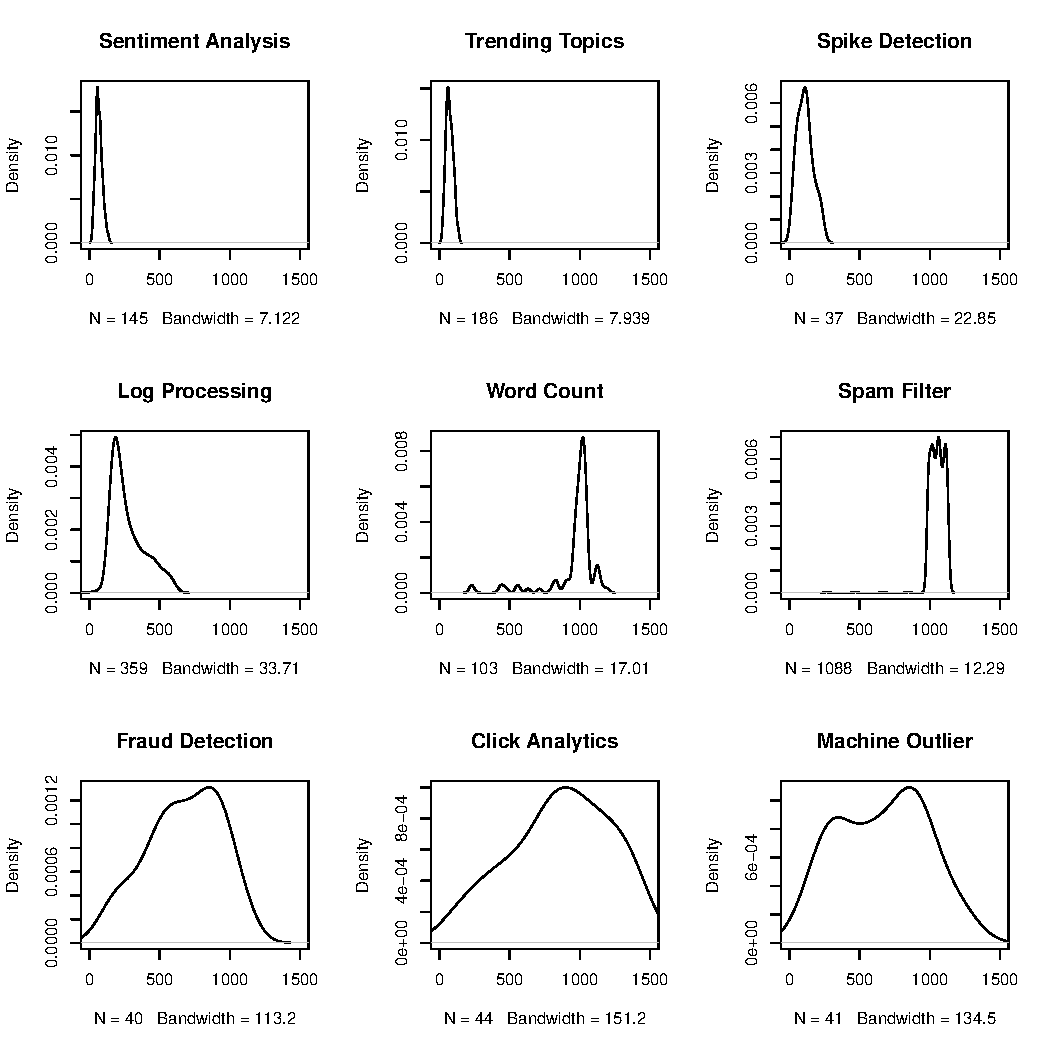
\includegraphics[width=.8\textwidth]{images/memory_usage.pdf}
	\caption{Memory usage per application (in MBytes)}
	\label{fig:memory_usage}
\end{figure}

As the SPSs store all the data in memory to reduce the latency, it is important to have applications with different patterns of memory usage for the benchmark suite. In the Figure \ref{fig:memory_usage} it is possible to see the distribution of the memory usage, measured at fixed time intervals during the application execution. The x-axis shows the amount of memory (in bytes) used, while the y-axis shows the density of occurrences. The selected applications exhibit five memory behaviours: fixed and variable memory usage; and low, medium and high memory usages.

%A broad base means an application with high variation of memory usage, while a narrow one means the memory consumption remains fixed or very limited.

The last characteristic observed was the time for an operator to process one tuple. The results shown in Figure \ref{fig:process_time} correspond to the 99th percentiles obtained from samples retrieved at fixed time intervals. There are applications with homogeneous processing times across operators, while others have bigger differences between operators. The highest processing time comes from the \emph{tokenizer} operator (\emph{spam filter}), which can be explained by the high selectivity of the operator.

\begin{figure}[ht!]
    \centering
	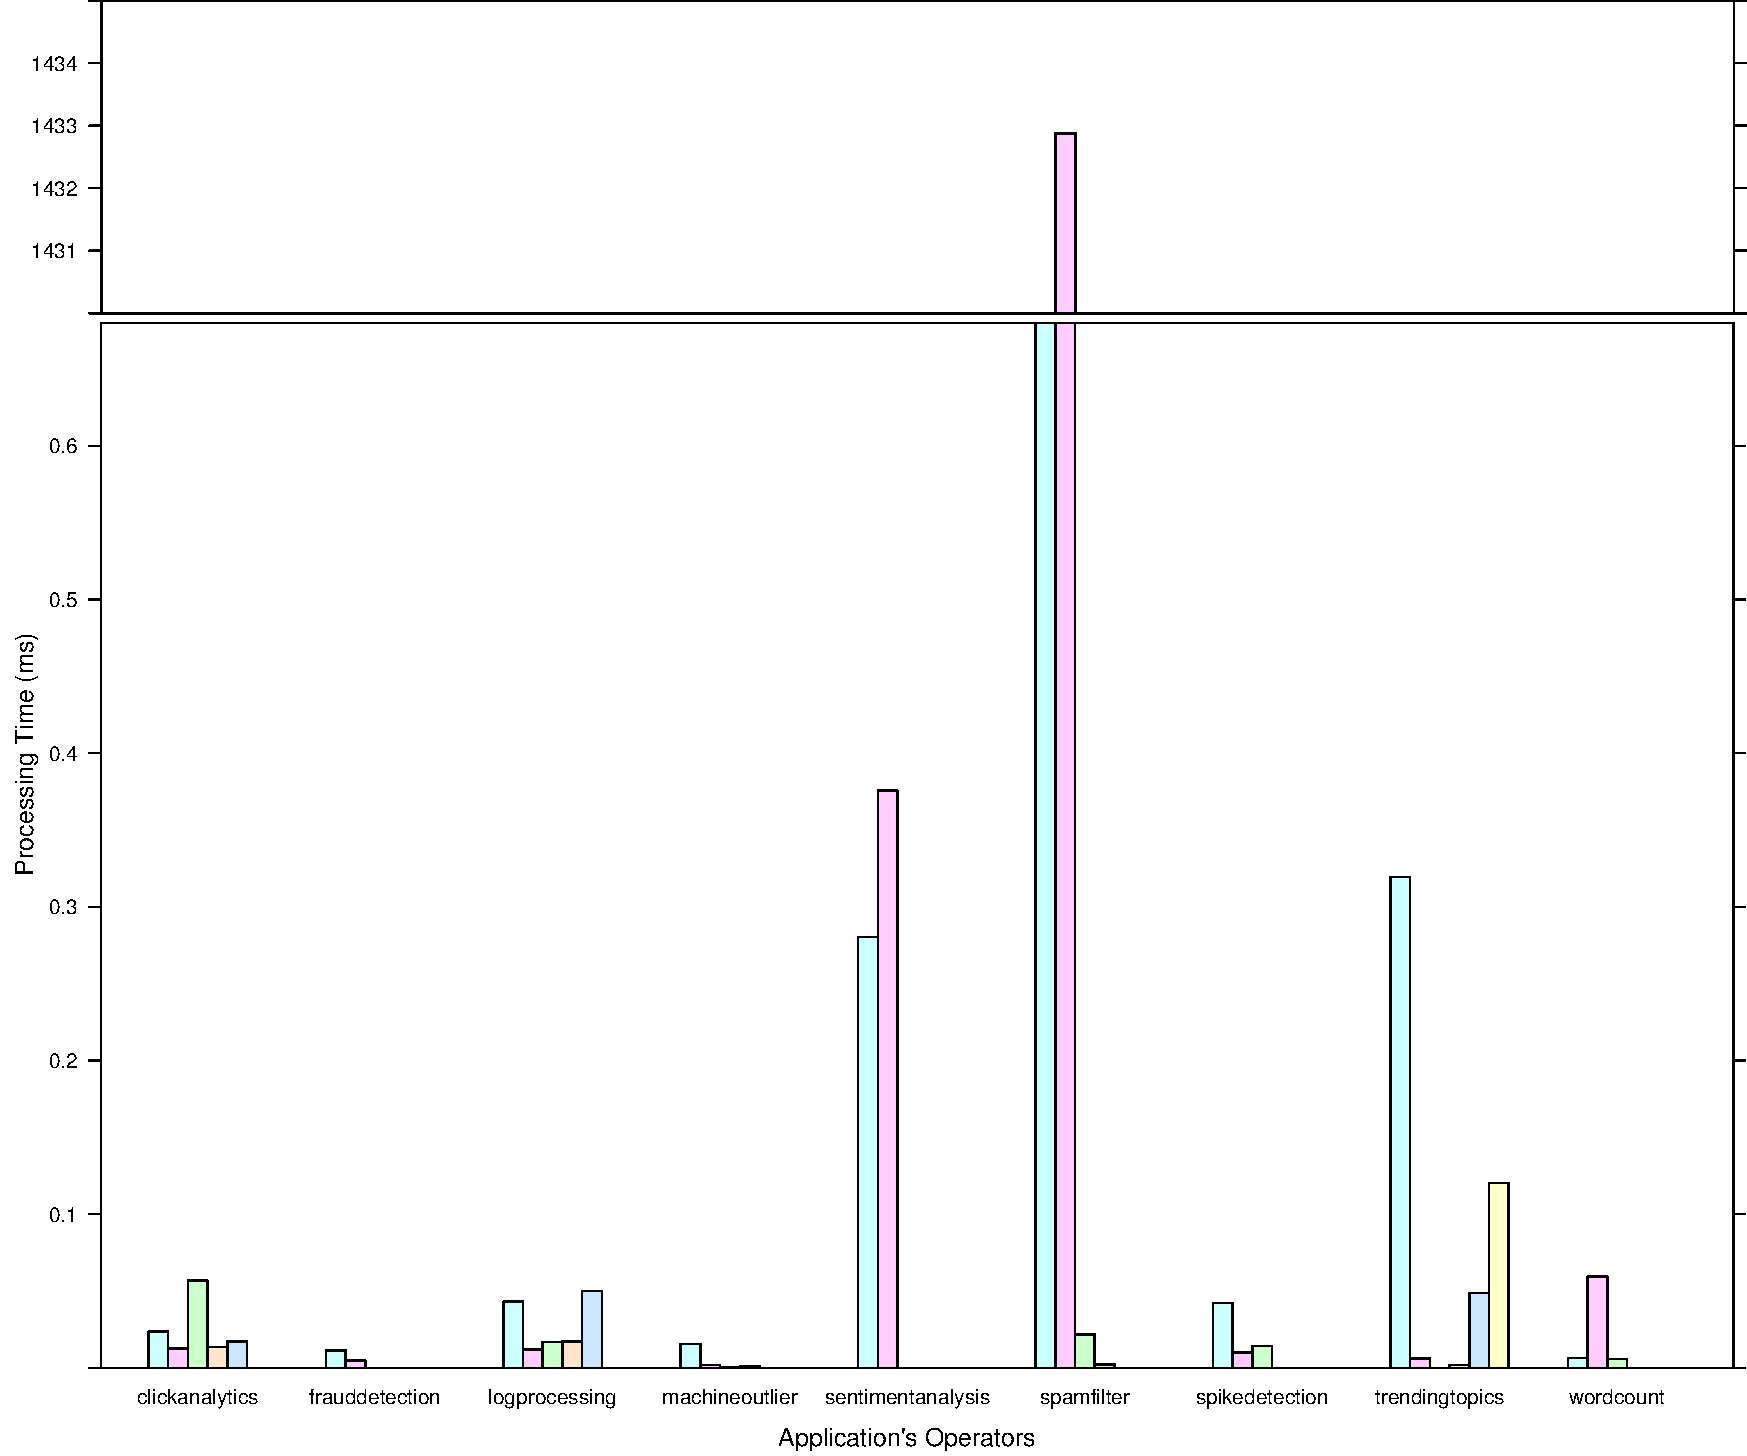
\includegraphics[width=.8\textwidth]{images/process_time.pdf}
	\caption{Process time per tuple per operator}
	\label{fig:process_time}
\end{figure}

\begin{table}[h]
\begin{center}
	\footnotesize
	\begin{tabular}{ | l | p{2.5cm} | p{2.5cm} | p{2cm} | l | l | l | p{1.5cm} | }
    		\hline
    		\textbf{App} & \textbf{Area} & \textbf{Operator} & \textbf{Type} & \textbf{Mem.} & \textbf{Sel.} & \textbf{Time} & \textbf{Comm.} \\ \hline
    		\multirow{2}{*}{WC} & \multirow{2}{*}{Text Processing} & SplitSentence & Projector & 1   & - & $N$ & Group By \\\cline{3-8}
    					        &                                  & WordCount     & Aggregator & $W$ & - & $N$ & Group By \\\hline
    					                
%    		\multirow{2}{*}{TT} & \multirow{2}{*}{Social Network} & SplitSentence & Projector? & 1   & ? & ? & Group By \\\cline{3-8}
%    					        &                                 & WordCount     & Aggregator & $W$ & ? & ? & Group By \\\hline
    					                  
    		\multirow{2}{*}{BI} & \multirow{2}{*}{Finance} & VWAP         & Group By Aggregator & $S$ & - & $N$ & Group By \\\cline{3-8}
    					        &                          & BargainIndex & Stream Join         & $S$ & - & $N$ & Shuffle \\\hline
    					                   
    		\multirow{2}{*}{SD} & \multirow{2}{*}{Sensor Network} & MovingAverage  & Group By Aggregator & $D$ & - & $N$ & Group By \\\cline{3-8}
    					        &                                 & SpikeDetector  & Select              & $1$ & - & $N$ & Shuffle \\\hline
    					                   
%    		\multirow{2}{*}{SA} & \multirow{2}{*}{\parbox[t]{2.5cm}{Natural Language Processing}} & StateLocator         & Projector & $1$ & ? & ? & Group By \\\cline{3-8}
%    					        &                                                                 & Sentiment Calculator  & Join      & $1$ & ? & ? & Shuffle \\\hline
    					                   
    		\multirow{1}{*}{FD} & \multirow{1}{*}{Finance} & Predictor & Select & $Uw$ & - & $N$ & Shuffle \\\hline
    		
    		\multirow{2}{*}{MO} & \multirow{2}{*}{\parbox[t]{2.5cm}{Network\\Monitoring}} & ObservationScore & Group By Aggregator & $r$  & - & $Nr$ & Group By \\\cline{3-8}
    					        &                                                         & AnomalyScore     & Group By Aggregator & $Mw$ & - & $N$ & Shuffle \\\cline{3-8}
    					        &                                                         & AlertTrigger     & Select              & $r$  & - & $Nr$ & Shuffle \\\hline
    					        
    		\multirow{1}{*}{RL} & \multirow{1}{*}{Advertising} & Reinforcement Learner & Stream Join & $m|S||A|$ & - & $N$ & Shuffle \\\hline
    		
    		\multirow{2}{*}{CA} & \multirow{2}{*}{\parbox[t]{2.5cm}{Web Analytics}} & RepeatVisit    & Group By Aggregator & $\sum_{i=0}^{U}v_{i}$  & - & $N$ & Shuffle \\\cline{3-8}
    					        &                                                   & VisitStats     & Aggregator          & $1$                    & - & $N$ & Shuffle \\\cline{3-8}
    					        &                                                   & LocationFinder & Join                & $1$                    & - & $N$ & Group By \\\cline{3-8}
    					        &                                                   & GeoStats       & Group By Aggregator & $C + T$                & - & $N$ & Shuffle \\\hline
    					        
    		\multirow{2}{*}{LP} & \multirow{2}{*}{\parbox[t]{2.5cm}{Web Analytics}} & VolumeCount    & Projector 	       & $1$  & - & $N$ & Shuffle \\\cline{3-8}
    					        &                                                   & IPStatusParser & Projector           & $1$  & - & $N$ & Shuffle, Group By \\\cline{3-8}
    					        &                                                   & Status Counter & Group By Aggregator & $S$  & - & $N$ & Shuffle \\\cline{3-8}
    					        &                                                   & IPLocation     & Join                & $1$  & - & $N$ & Group By \\\cline{3-8}
    					        &                                                   & CountryStatus  & Join                & $C + T$  & $N$ & - & Group By \\\hline
    					        
    		\multirow{2}{*}{SF} & \multirow{2}{*}{\parbox[t]{2.5cm}{--}} & Tokenizer       & Projector       & $1$             & - & $N$ & Group By \\\cline{3-8}
    					        &                                        & WordProbability & Join            & $W$             & - & $N$ and $NW$ & Group By \\\cline{3-8}
    					        &                                        & BayesRule       & Join Aggregator & $\overline{M}$  & - & $N$ & Shuffle \\\hline
    		
	\end{tabular}
	\caption{Applications characterization}
	\label{table:app_characteristics}
	
\end{center}
\end{table}

% Tuple size: fixed or variable
% Data type: text, numeric, multimedia (audio, video, image)
% Operator type: stateless or stateful (non-blocking, windowed, aproximate)



\section{Configuration and Datasets}
\label{sec:configuration_datasets}

This section describes in detail the recommended datasets to be used by the selected applications seen in Section \ref{sec:applications}. Most of the datasets consists of data from real-world scenarios. In the case of the \emph{Fraud Detection} and \emph{Reinforcement Learner} a dataset has not been found, instead a generator has to be used.

There are also cases where the size of the dataset is not big enough, i.e. the dataset can be consumed by the application in a matter of minutes, requiring it to be replicated until its size is acceptable. The amount of time required to consume a dataset is very subjective, and will be influenced by the plataform in which the application is running as well as the infrastructure where the platform has been deployed. The StreamBench \cite{lu2014stream}, for example, uses datasets with the number of records in the order of millions.

It is important to note that replicating a dataset is not always as simple as making copies of it. There are cases where some data fields have to be changed in order not to break the semantics of the application. In the case of the applications that compose this benchmark suite, the datasets that have date fields must be altered in order to follow continuous timeline, instead of going back and forth if the dataset were simply duplicated.

\begin{table*}[t]
\begin{center}
	\footnotesize
	\begin{tabular}{ | l | l | c | c |}
   		\hline
		\textbf{Application} & \textbf{Dataset} & \textbf{Size} & \textbf{Comments} \\ \hline
		
        \multirow{2}{*}{Word Count} & Project Gutenberg \footnote{http://www.gutenberg.org/} & ~8GB & \\\cline{2-4}
        & Wikipedia Dumps \footnote{https://dumps.wikimedia.org/} & ~9GB & text only \\\hline
        
        Log Processing / Click Analytics & 1998 World Cup \footnote{http://ita.ee.lbl.gov/html/contrib/WorldCup.html} & 104GB & \\\hline
        \multirow{2}{*}{Traffic Monitoring} & Beijing Taxi Traces \footnote{http://anrg.usc.edu/www/downloads/} & 280MB & \\\cline{2-4}
        & Dublin Bus Traces & 4GB & \\\hline
        
        Machine Outlier & Google Cluster Traces \footnote{http://code.google.com/p/googleclusterdata/} & 36GB & \\\hline
        Sentiment Analysis / Trending Topics & Twitter Streaming API \footnote{https://dev.twitter.com/docs/api/streaming} & - & \\\hline
        Fraud Detection & \emph{generated} & - & \\\hline
        Spike Detection & Intel Berkeley Research Lab \footnote{http://db.csail.mit.edu/labdata/labdata.html} & 150MB & \\\hline
        Bargain Index & Yahoo Finance \footnote{https://finance.yahoo.com/}, Google Finance \footnote{https://www.google.com/finance} & - & \\\hline
        Reinforcement Learner & \emph{generated} & - & \\\hline
        
        \multirow{4}{*}{Spam Filter} & TREC 2007 \footnote{http://plg.uwaterloo.ca/~gvcormac/spam/} & 547MB & labeled \\\cline{2-4}
        & SPAM Archive \footnote{http://untroubled.org/spam/} & ~1.2GB & spam only\\\cline{2-4}
        & Enron Email Dataset \footnote{http://www.cs.cmu.edu/~./enron/} & 2.6GB & raw \\\cline{2-4}
        & Enron Spam Dataset \footnote{http://nlp.cs.aueb.gr/software\_and\_datasets/Enron-Spam/index.html} & 50MB & labeled\\\hline
        
        Smart Grid Monitoring & DEBS Grand Challenge 2014 & 100GB & \\\hline
        
	\end{tabular}
	\vspace{5px}
	\caption{Application's datasets}
	\label{table:app_datasets}
\end{center}
\end{table*}

One of the main factors that has to be explored is the parallelism of the operators. There has to be a thorough planning of the applications that are going to be executed and the amount of time available for executing the experiments, in order to select a reasonable number of combinations for the parallelism.

Still, there is the matter of selecting the configurations that will display the best performance in therms of throughput and latency. Depending on the platform, increasing the parallelism may incur in an increase in memory usage, which will at some point lead to loss of performance and even errors.

One approach taken by this work is to calculate the weighted average of processing time required for one tuple for each operator in relation to the overall processing time of one tuple for the application. The importance of the selectivity of operators can be seen here, as it is the weight that indicates how many tuples it generates with one tuple given as input.

Given an application with $N_{op}$ operators, each with $N_{in}$ input streams, the score of each operator $s_{op}$ is given by Equation \ref{eq:parallelism_score}, with $T_{p_{i}}$ as the 99th percentile for the processing time of one tuple at the operator $i$ and $S_{in_{i}}$ the selectivity of the upstream operator that generated the input stream.

With the score of all operators calculated, the score of the application $s_{app}$ is the sum of the scores of the operators. At last, to calculate the number of instances per operator $I_{op_{i}}$, the score of the operator is multiplied by $10$ and divided by the score of the app, the result is rounded up to the nearest integer so that the operator has at least one instance.

\begin{equation}\label{eq:parallelism_score}
  \begin{aligned}
  s_{op} = \sum_{i=1}^{N_{in}}T_{p_{i}} \times S_{in_{i}} \\
  s_{app} = \sum_{i=1}^{N_{op}}s_{op_{i}} \\
  I_{op_{i}} = ceil(\frac{s_{op_{i}} \times 10}{s_{app}})
  \end{aligned}
\end{equation}

With the number of instances at hand (see Table \ref{table:app_parallelism}), it can be used as one of the configurations for the application. To experiment with more configurations these numbers can be used as a base and a set of multipliers can be selected in order to try configurations with a greater level of parallelism.

The second approach, much simpler than the first, consists of giving one instances for all operators and then selecting the multipliers. And in a third one the number generated in the first approach is used, but instead of multiplying all operators, only the parallelism of the source is increased.

There is another approach that has not been used in this work, which is simulation. It could be an interesting approach as it could try many more configurations. In any case, the fact is that it would be impossible to try all the possible combinations, and there is also no guarantee that one configuration will behave in the same way in different platforms.

\begin{table*}[t]
\begin{center}
	\footnotesize
\begin{tabular}{ | l | l | l | }
\hline
	Application & Operator & Instances \\ \hline
	word-count & source & 1 \\ \hline
	 & splitter & 5 \\ \hline
	 & counter & 6 \\ \hline
	 & sink & 3 \\ \hline
	log-processing & source & 4 \\ \hline
	 & status-counter & 1 \\ \hline
	 & volume-counter & 2 \\ \hline
	 & geo-locator & 4 \\ \hline
	 & geo-summarizer & 2 \\ \hline
	 & sink & 4 \\ \hline
	traffic-monitoring & source & 1 \\ \hline
	 & map-matcher & 2 \\ \hline
	 & speed-calculator & 2 \\ \hline
	 & sink & 1 \\ \hline
	machine-outlier & source & 6 \\ \hline
	 & scorer & 1 \\ \hline
	 & anomaly-scorer & 1 \\ \hline
	 & alert-trigger & 4 \\ \hline
	 & sink & 1 \\ \hline
	spam-filter & source & 1 \\ \hline
	 & tokenizer & 10 \\ \hline
	 & word-probability & 1 \\ \hline
	 & bayes-rule & 1 \\ \hline
	 & sink & 1 \\ \hline
	sentiment-analysis & source &  \\ \hline
	 & tweet-filter &  \\ \hline
	 & text-filter &  \\ \hline
	 & stemmer &  \\ \hline
	 & positive-scorer &  \\ \hline
	 & negative-scorer &  \\ \hline
	 & joiner &  \\ \hline
	 & scorer &  \\ \hline
	 & sink &  \\ \hline
	trending-topics & source & 9 \\ \hline
	 & topic-extractor & 2 \\ \hline
	 & counter & 1 \\ \hline
	 & intermediate-ranker & 1 \\ \hline
	 & total-ranker & 1 \\ \hline
	 & sink & 1 \\ \hline
	click-analytics & source & 2 \\ \hline
	 & repeat-visits & 2 \\ \hline
	 & total-visits & 2 \\ \hline
	 & geo-locator & 5 \\ \hline
	 & geo-summarizer & 1 \\ \hline
	 & sink-visits & 1 \\ \hline
	 & sink-locations & 1 \\ \hline
	fraud-detection & source & 8 \\ \hline
	 & predictor & 3 \\ \hline
	 & sink & 2 \\ \hline
	spike-detection & source & 7 \\ \hline
	 & moving-average & 3 \\ \hline
	 & spike-detector & 2 \\ \hline
	 & sink & 1 \\ \hline
\end{tabular}
	\caption[Number of instances of operators]{Number of instances of operators based on the weighted average of processing time.}
	\label{table:app_parallelism}
\end{center}
\end{table*}

% -----------------------------------------------------------------------------
\chapter{Results}
\label{chapter:results}

This chapter presents the results obtained by applying the benchmark model defined on Chapter \ref{chapter:model} in the comparison of two of main stream processing systems in the market against a subset of the applications defined.

The SPSs chosen were Spark and Storm as they are the most prominent on their category and also because they have different approaches on how to handle stream data processing.

Out of the 14 applications defined, due to time restrictions to the cluster for running the experiments, 3 were chosen: word count, log processing and traffic monitoring. The first one has become a standard in Big Data benchmarks, while the second has a good set of operations applied to logs as well as having the biggest dataset available at the time. And the third application is a convergence of IoT and Big Data applied to what is know as \textit{Smart Cities}.

\section{Set-Up}
\label{sec:set-up}

The experiments were executed in the Azure cloud computing service with a cluster of 8 computing instances, one master instance and 3 data instances, all of type \textit{Medium} (Standard\_A2) running Ubuntu Server 12.04. The configuration of those instances is described on Table \ref{table:azure_medium_config}.

\begin{table*}[h]
\centering
\caption{My caption}
\label{my-label}
\begin{tabular}{lllll}
\hline
\textbf{CPU Cores}                & 2        &  &  &  \\ \hline
\textbf{Memory}                   & 3.5 GB   &  &  &  \\ \hline
\textbf{Local HDD}                & 135 GB   &  &  &  \\ \hline
\textbf{Max data disk throughput} & 500 IOPS &  &  &  \\ \hline
\end{tabular}
\caption{Azure Medium instance configuration.}
	\label{table:azure_medium_config}
\end{table*}

The message system employed for the experiments was Apache Kafka 0.8.1.1 (Scala 2.9.2) installed on the 3 data instances of the cluster. The data producers that fed Kafka were also installed on the data instances, thus avoiding network traffic.

Each data instance had one data producer reading data from a separate hard disk and forwarding it to Kafka. On the application side, the number of Kafka partitions always matched the number of instances of the source operator.

The Spark version used on the experiments was 1.3.1 on top of Hadoop YARN 2.6. And for Storm it was version 0.9.2 running on top of Supervisord. Storm also depends on Zookeeper for coordination, in the cluster version 3.4.6 was installed on the master instance, plus two of the three data instances.

\begin{figure}[h]
    \centering
	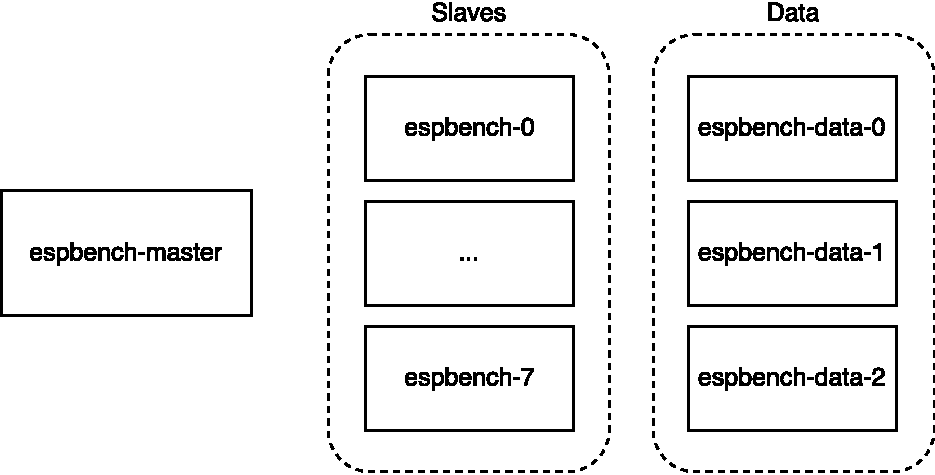
\includegraphics[width=.8\textwidth]{images/cluster_azure.pdf}
	\caption{Cluster Azure}
	\label{fig:cluster_azure}
\end{figure}



% Environment, message system, configurations, etc, etc...

\section{Word Count}

For the \textit{word count} on Storm, 52 different configurations of number of instances of operators were tried. While on Spark only 12 of those 52 configurations were able to run effectively.

Each configuration is identified by \textbf{n\textit{N}}\_\textbf{x\textit{Source}}\_\textbf{x\textit{Splitter}}\_\textbf{x\textit{Counter}}\_\textbf{x\textit{Sink}} which is the number of nodes and the number of instances of each operator. If only one \textbf{x\textit{X}} is defined, it means all operators have the same number of instances.

When analysing the 95th percentile of latency results on Storm some experiments showed extremely high latencies as shown on Figure \ref{fig:storm_wordcount_latency}.

\begin{figure}[H]
    \centering
	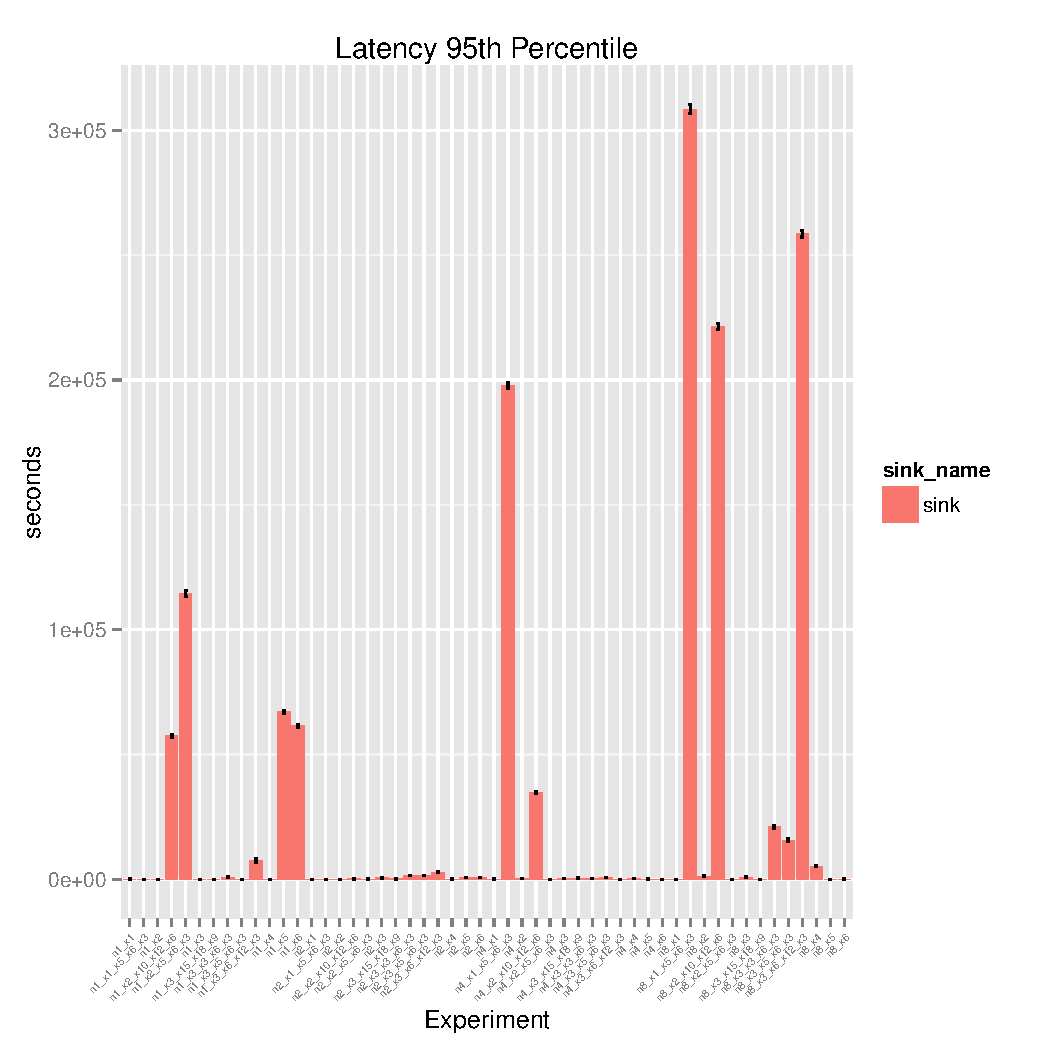
\includegraphics[width=.6\textwidth]{summaries/storm_wordcount/full_latency.pdf}
	\caption{Storm Word Count Latencies}
	\label{fig:storm_wordcount_latency}
\end{figure}

Looking more closely, the best experiments managed to perform latencies under 15 seconds as the Figure \ref{fig:storm_wordcount_latency_best} shows. The best one was \textbf{n2\_x1} with a latency of 7.2 seconds, followed by \textbf{n2\_x1\_x5\_x6\_x3} with 9.9 seconds.

\begin{figure}[H]
    \centering
	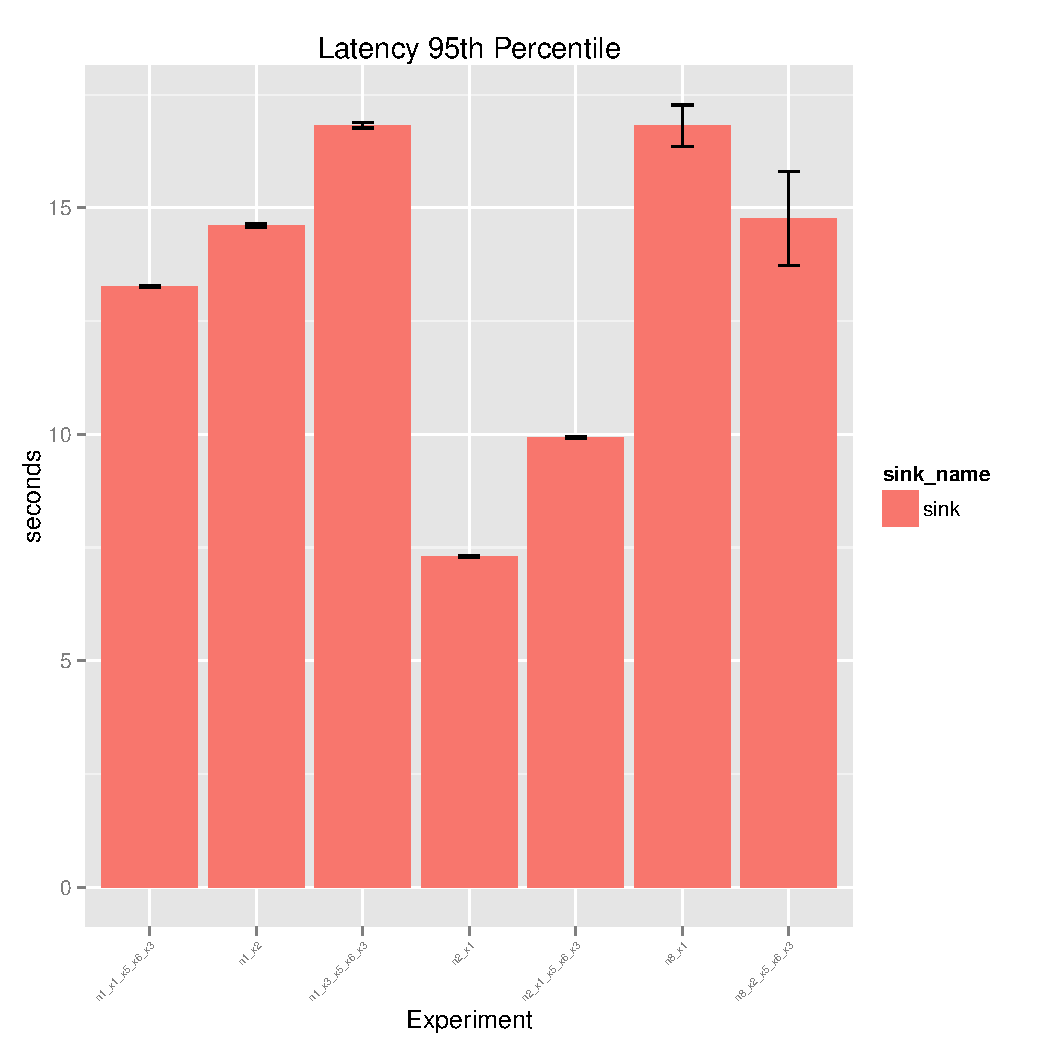
\includegraphics[width=.6\textwidth]{summaries/storm_wordcount/full_best_latency.pdf}
	\caption{Storm Word Count Best Latencies}
	\label{fig:storm_wordcount_latency_best}
\end{figure}

When looking at the throughput average on Figure \ref{fig:storm_wordcount_throughput}, the best results occur on the experiments with 8 nodes. The best one (\textbf{n8\_x4}) was able to deliver an average of 95k tuples per second on the splitter and counter, and 94k on the sink, which is the throughput of results.

\begin{figure}[H]
    \centering
	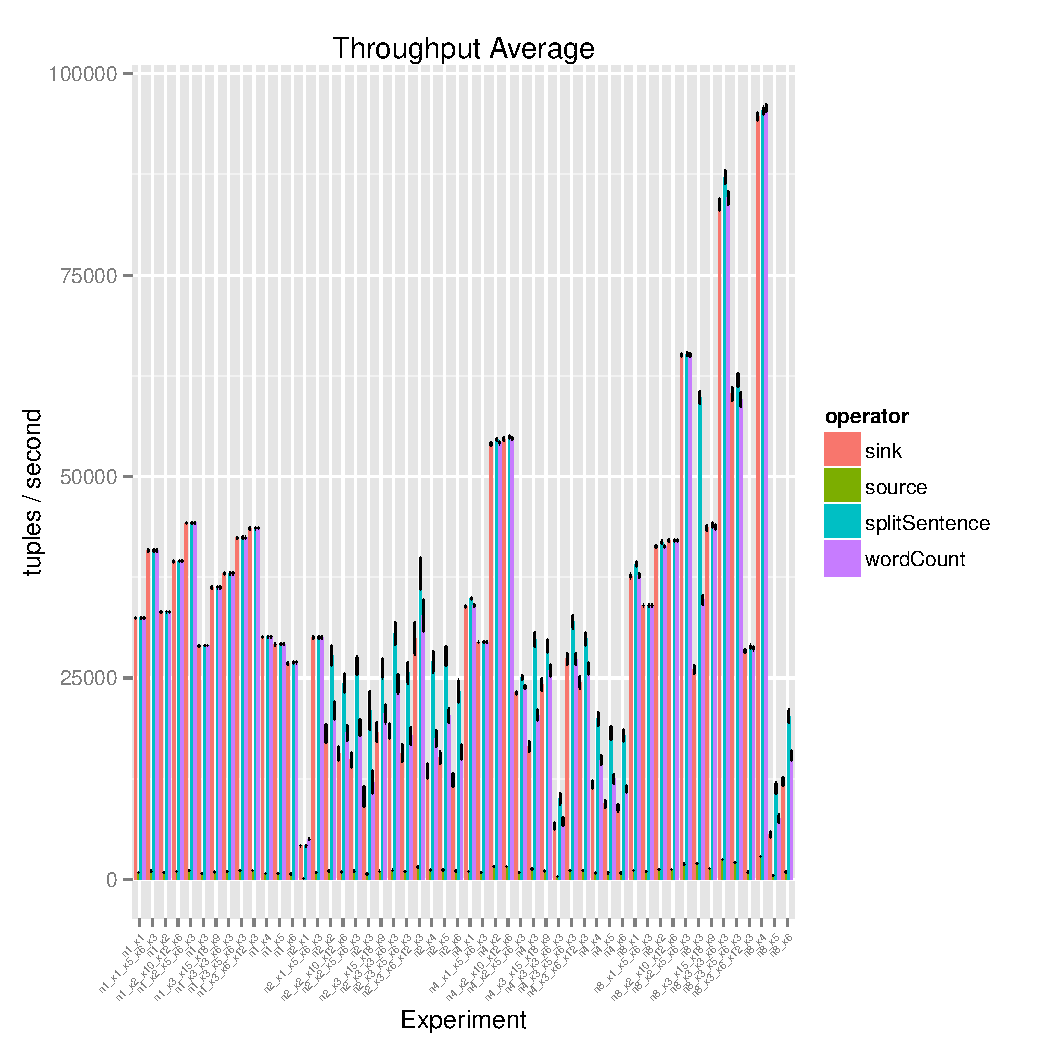
\includegraphics[width=.6\textwidth]{summaries/storm_wordcount/full_throughput.pdf}
	\caption{Storm Word Count Throughput}
	\label{fig:storm_wordcount_throughput}
\end{figure}

The network usage average on Figure \ref{fig:storm_wordcount_network} shows that as the number of nodes increases the network activity also increases. Experiments with one and two nodes show very minimal network usage.

\begin{figure}[H]
    \centering
	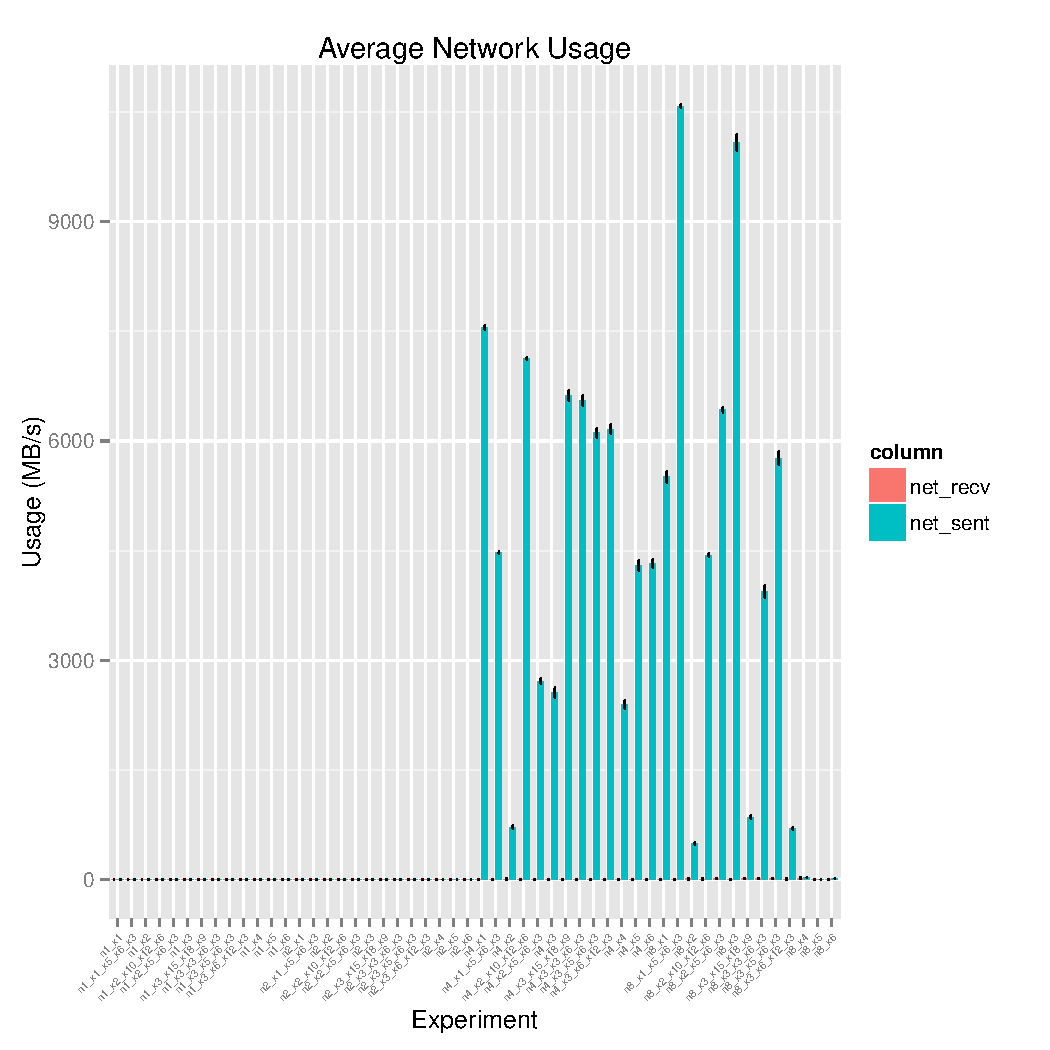
\includegraphics[width=.6\textwidth]{summaries/storm_wordcount/full_network.pdf}
	\caption{Storm Word Count Network Usage}
	\label{fig:storm_wordcount_network}
\end{figure}

The CPU and memory usage are displayed on Figure \ref{fig:storm_wordcount_cpu_mem}. Some of the experiments failed to correctly measure the CPU usage.

\begin{figure}[H]
    \centering
	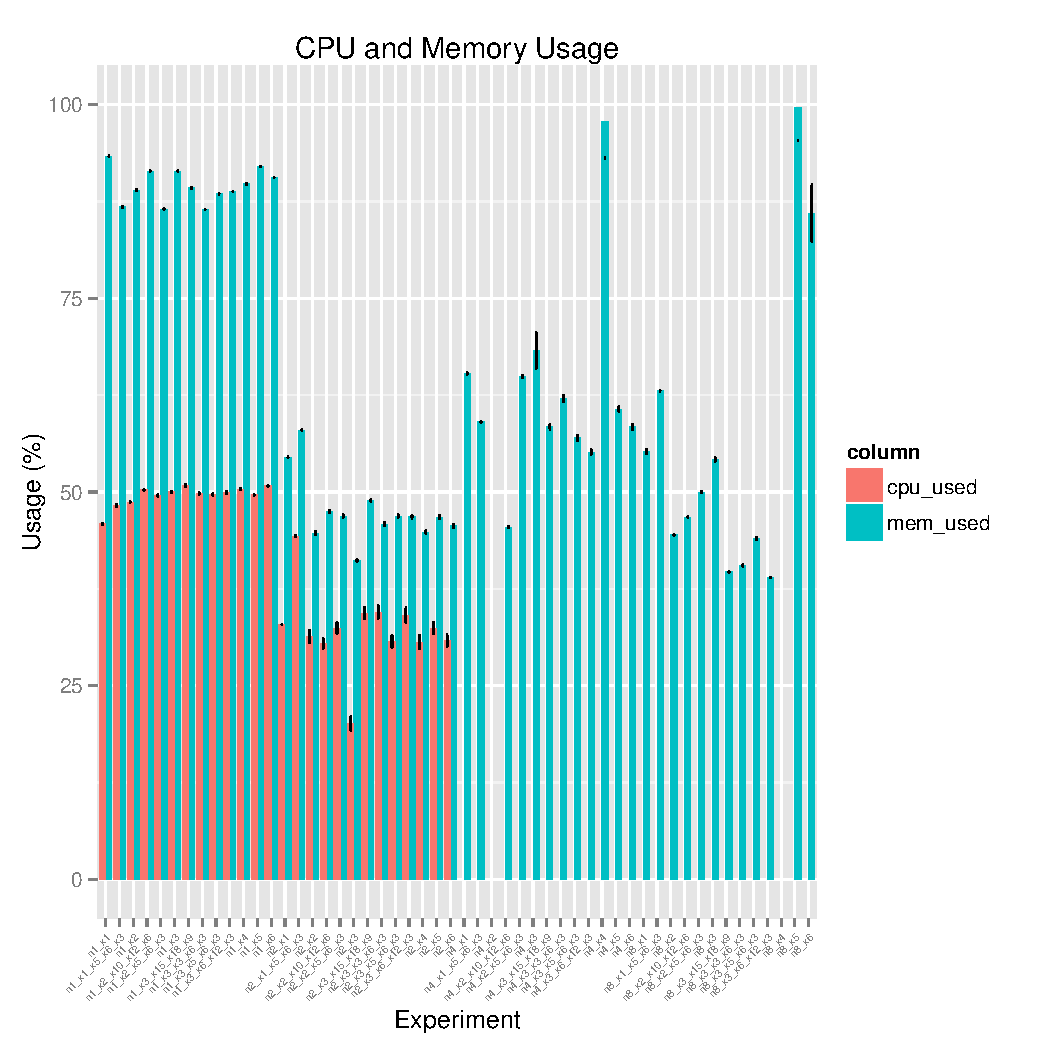
\includegraphics[width=.6\textwidth]{summaries/storm_wordcount/full_cpu_mem.pdf}
	\caption{Storm Word Count CPU and Memory Usage}
	\label{fig:storm_wordcount_cpu_mem}
\end{figure}

On Spark the 95th percentile of latencies (Figure \ref{fig:spark_wordcount_latency}) were more stable, with results ranging from 20 to 40 seconds. The batch size of the applications was configured to 1 second.

\begin{figure}[H]
    \centering
	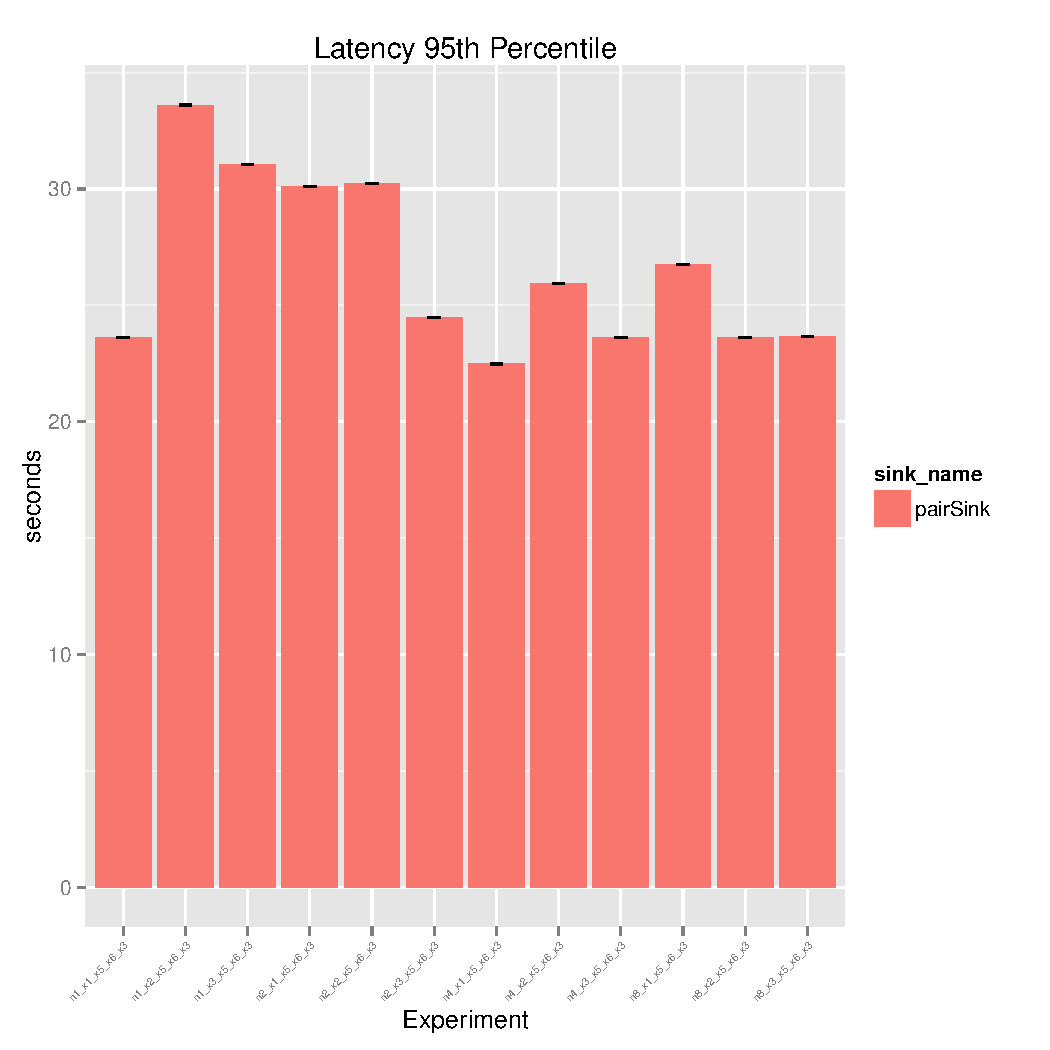
\includegraphics[width=.6\textwidth]{summaries/spark_wordcount/latency.pdf}
	\caption{Spark Word Count Latencies}
	\label{fig:spark_wordcount_latency}
\end{figure}

The average throughput of the applications (Figure \ref{fig:spark_wordcount_throughput}) were inferior to Storm, but they were more stable. On the sink, however, the throughput was much lower, with results ranging from 2897 tuples per second on experiment \textbf{n1\_x1\_x5\_x6\_x3} and 3933 tuples per second on experiment \textbf{n4\_x3\_x5\_x6\_x3}.

\begin{figure}[H]
    \centering
	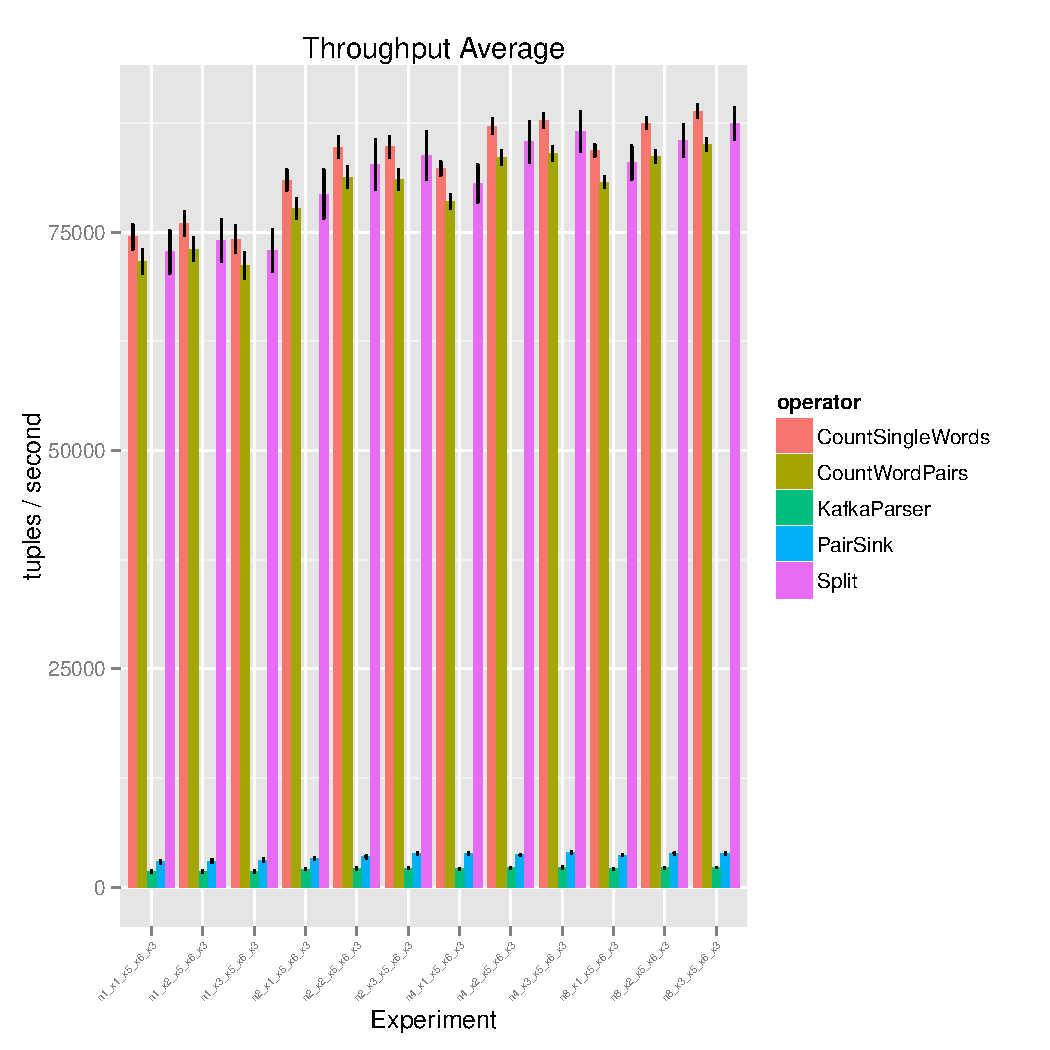
\includegraphics[width=.6\textwidth]{summaries/spark_wordcount/throughput.pdf}
	\caption{Spark Word Count Throughput}
	\label{fig:spark_wordcount_throughput}
\end{figure}

The network usage, on Figure \ref{fig:spark_wordcount_network}, also showed a more stable increase as the number of nodes were increased.

\begin{figure}[H]
    \centering
	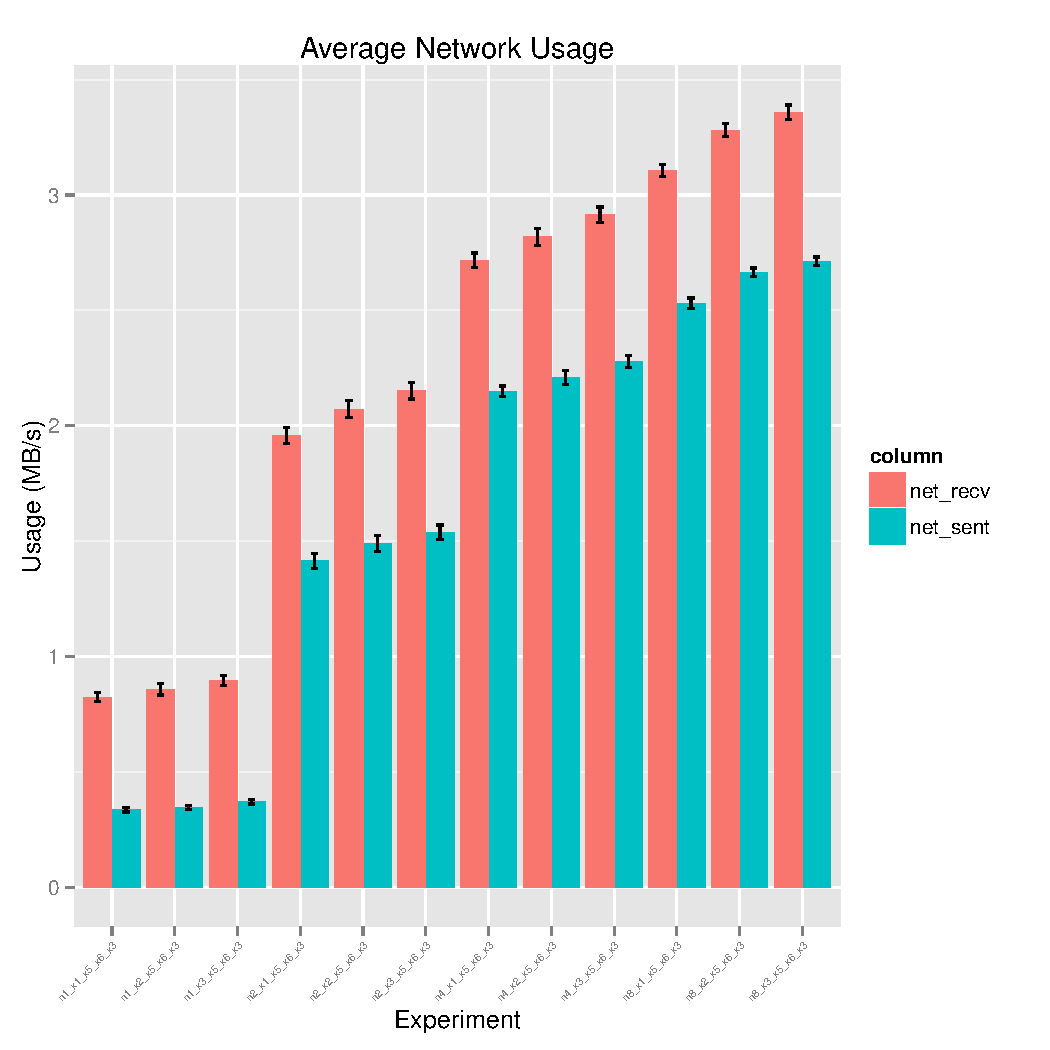
\includegraphics[width=.6\textwidth]{summaries/spark_wordcount/network.pdf}
	\caption{Spark Word Count Network Usage}
	\label{fig:spark_wordcount_network}
\end{figure}

The CPU usage on the Spark applications shown on Figure \ref{fig:spark_wordcount_cpu_mem} decreased as the number of nodes increased, while the memory reached its peak at 90\% on experiment \textbf{n4\_x1\_x5\_x6\_x3} and then decreased slightly.

\begin{figure}[H]
    \centering
	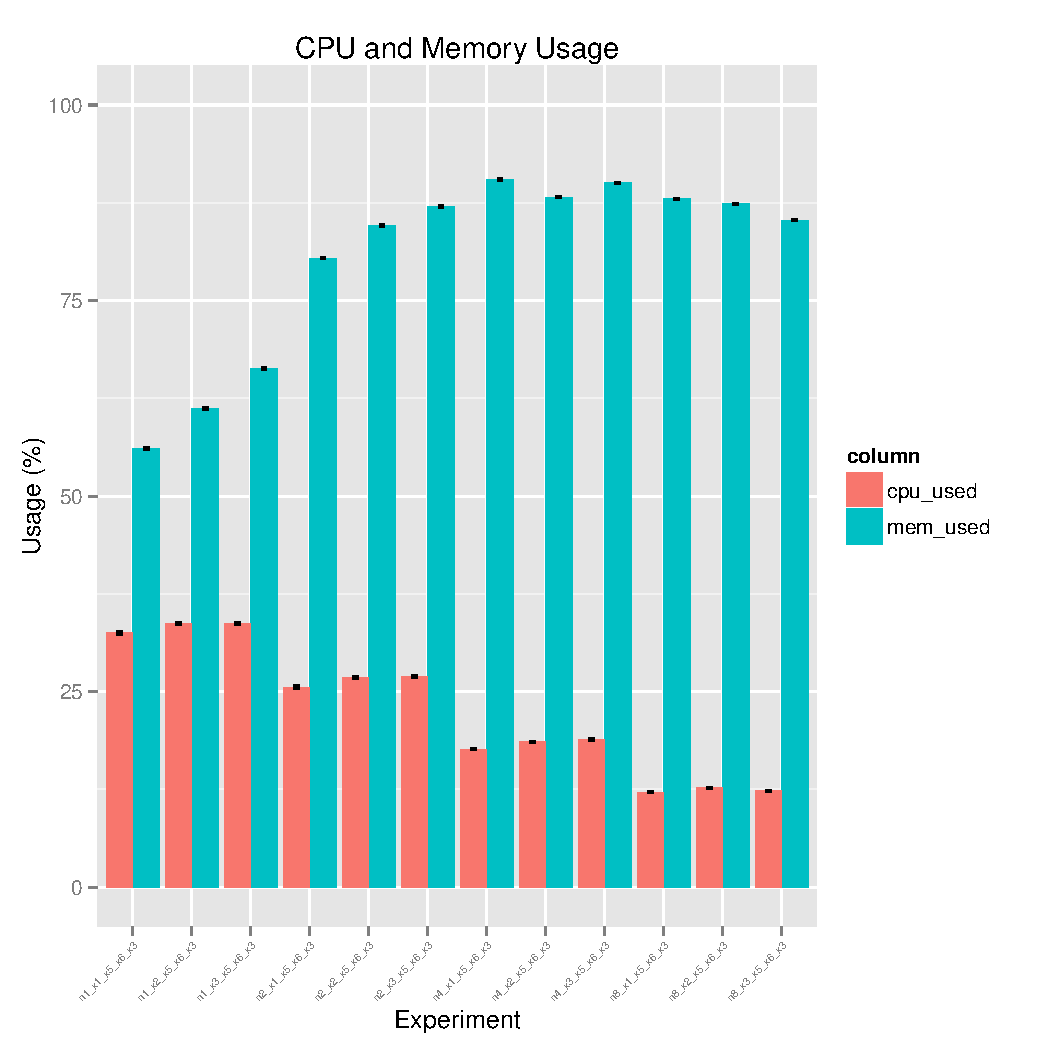
\includegraphics[width=.6\textwidth]{summaries/spark_wordcount/cpu_mem.pdf}
	\caption{Spark Word Count CPU and Memory Usage}
	\label{fig:spark_wordcount_cpu_mem}
\end{figure}

In general, Storm had a better performance than Spark, with better results for throughput and latency, the latter was expected because of the batching of tuples that happens on Spark. On the other hand, Spark seemed more stable regarding the usage of resources.

\begin{table}[H]
\tiny
\centering
\caption{Comparison of Word Count results}
\label{table:comparison_wordcount}
\begin{tabular}{|l|l|l|l|}
\hline
Platform & Experiment & Latency (ms) & Throughput (tps)\\ \hline
Spark    &                                      & 23625.82965848                           & 2897.58773878276                         \\ \cline{1-1} \cline{3-4} 
Storm    & \multirow{-2}{*}{n1\_x1\_x5\_x6\_x3} & \cellcolor[HTML]{34E570}13273.488994646  & \cellcolor[HTML]{34E570}40859.5828991725 \\ \hline
Spark    &                                      & \cellcolor[HTML]{34E570}33603.3111416812 & 2999.1589673913 \\ \cline{1-1} \cline{3-4} 
Storm    & \multirow{-2}{*}{n1\_x2\_x5\_x6\_x3} & 114488877.09637                          & \cellcolor[HTML]{34E570}44232.99535501 \\ \hline
Spark    &                                      & 31052.7268609758                         & 3081.00826446281 \\ \cline{1-1} \cline{3-4} 
Storm    & \multirow{-2}{*}{n1\_x3\_x5\_x6\_x3} & \cellcolor[HTML]{34E570}16825.2406841784 & \cellcolor[HTML]{34E570}42383.2321259843 \\ \hline
Spark    &                                      & 30100.0515049                            & 3283.37426356589 \\ \cline{1-1} \cline{3-4} 
Storm    & \multirow{-2}{*}{n2\_x1\_x5\_x6\_x3} & \cellcolor[HTML]{34E570}9926.04326233308 & \cellcolor[HTML]{34E570}30046.043963401 \\ \hline
Spark    &                                      & \cellcolor[HTML]{34E570}30220.6235703883 & 3493.33747547417 \\ \cline{1-1} \cline{3-4} 
Storm    & \multirow{-2}{*}{n2\_x2\_x5\_x6\_x3} & 124921.308943089                         & \cellcolor[HTML]{34E570}14865.7479338843 \\ \hline
Spark    &                                      & \cellcolor[HTML]{34E570}24463.1167392591 & 3849.35728542914 \\ \cline{1-1} \cline{3-4} 
Storm    & \multirow{-2}{*}{n2\_x3\_x5\_x6\_x3} & 1521321.05084746                         & \cellcolor[HTML]{34E570}15664.8291666667 \\ \hline
Spark    &                                      & \cellcolor[HTML]{34E570}22485.5769731385 & 3828.1811422778 \\ \cline{1-1} \cline{3-4} 
Storm    & \multirow{-2}{*}{n4\_x1\_x5\_x6\_x3} & 197766604.967704                         & \cellcolor[HTML]{34E570}29408.880794018 \\ \hline
Spark    &                                      & \cellcolor[HTML]{34E570}25924.7815501678 & 3689.2752534079 \\ \cline{1-1} \cline{3-4} 
Storm    & \multirow{-2}{*}{n4\_x2\_x5\_x6\_x3} & 36072.407363065                          & \cellcolor[HTML]{34E570}23171.9327135203 \\ \hline
Spark    &                                      & \cellcolor[HTML]{34E570}23613.5836153283 & 3933.79567956796 \\ \cline{1-1} \cline{3-4} 
Storm    & \multirow{-2}{*}{n4\_x3\_x5\_x6\_x3} & 742380.394572025                         & \cellcolor[HTML]{34E570}27387.705370844 \\ \hline
Spark    &                                      & \cellcolor[HTML]{34E570}26752.1967323336 & 3681.78756420063 \\ \cline{1-1} \cline{3-4} 
Storm    & \multirow{-2}{*}{n8\_x1\_x5\_x6\_x3} & 308494259.645302                         & \cellcolor[HTML]{34E570}33996.4117473039 \\ \hline
Spark    &                                      & 23625.82965848                           & 3879.84336645237 \\ \cline{1-1} \cline{3-4} 
Storm    & \multirow{-2}{*}{n8\_x2\_x5\_x6\_x3} & \cellcolor[HTML]{34E570}14764.3578708167 & \cellcolor[HTML]{34E570}65082.6187793427 \\ \hline
Spark    &                                      & \cellcolor[HTML]{34E570}23647.8457369693 & 3858.31215970962 \\ \cline{1-1} \cline{3-4} 
Storm    & \multirow{-2}{*}{n8\_x3\_x5\_x6\_x3} & 15670409.7215233                         & \cellcolor[HTML]{34E570}60261.0911764706 \\ \hline
\end{tabular}
\end{table}

Latency = 95th percentile, Throughput = average, CPU and Memory Usage = average \%, Network Usage = average MBytes

Analysing Table \ref{table:comparison_wordcount}, Storm did better on throughput (won 12 out of 12 experiments), while Spark did better on latency (won 8 out of 12 experiments).




\section{Log Processing}

For the \textit{log processing} application, 44 different configurations were executed on Storm, and a subset of 16 on Spark.

Each configuration is identified by \textbf{n\textit{N}}\_\textbf{x\textit{Source}}\_\textbf{x\textit{VolumeCounter}}\_\textbf{x\textit{StatusCounter}}\\\_\textbf{x\textit{GeoFinder}}\_\textbf{x\textit{GeoStats}}\_\textbf{x\textit{VolumeSink}}\_\textbf{x\textit{StatusSink}}\_\textbf{x\textit{CountrySink}} which is the number of nodes and the number of instances of each operator. If only one \textbf{x\textit{X}} is defined, it means all operators have the same number of instances.

On Spark, due to its functional programming nature, some operators required actually two operators in order to first partitionate the tuples and then do the actual counting. Those were the \textit{volume counter}, \textbf{status counter}, and the \textbf{geofinder} and \textbf{geostats} were splitted into four operators: two for partitioning and counting cities, and two for partitioning and counting countries.

Looking at the 95th percentile of latencies for Storm on Figure \ref{fig:storm_logprocessing_latency}, there were some experiments with latencies beyond the acceptable.

\begin{figure}[H]
    \centering
	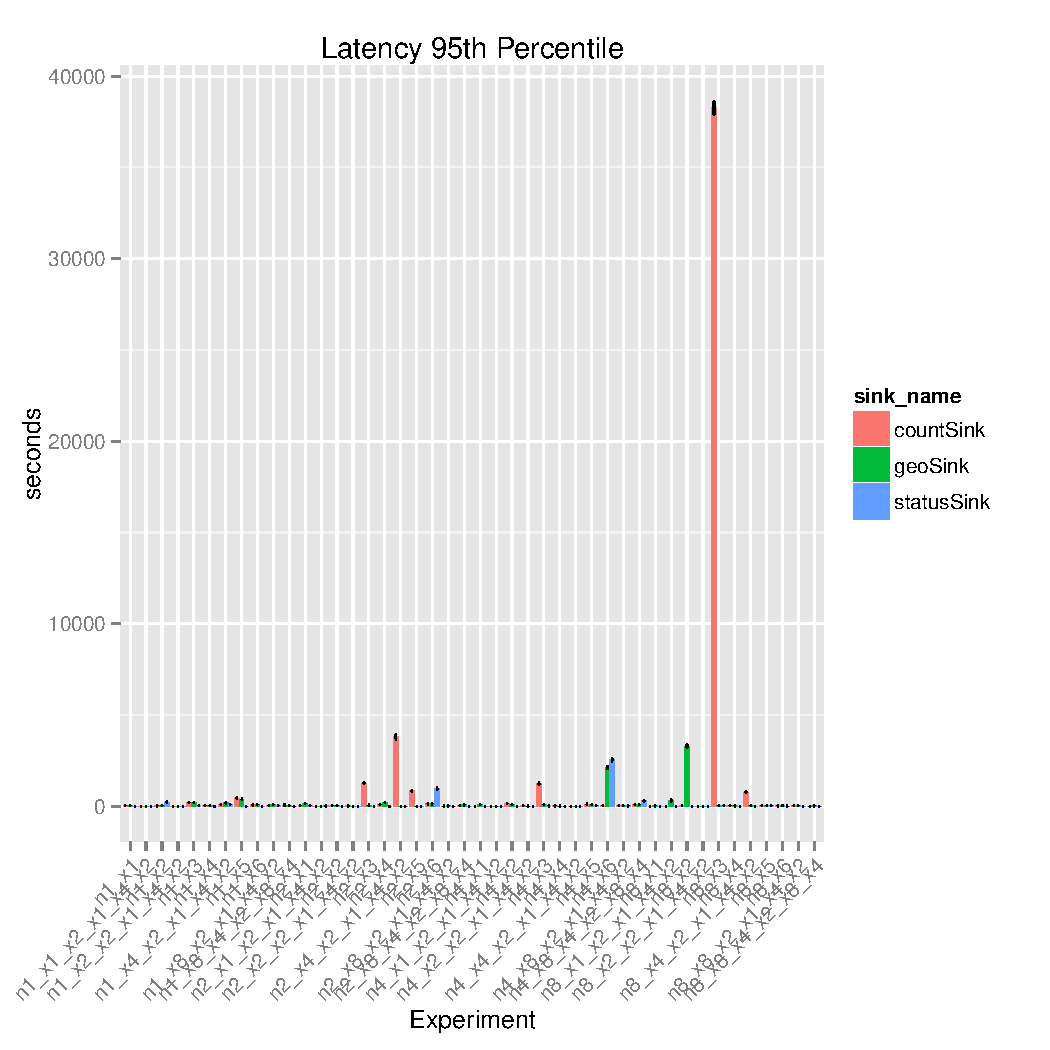
\includegraphics[width=.6\textwidth]{summaries/storm_logprocessing/full_latency.pdf}
	\caption{Storm Log Processing Latencies}
	\label{fig:storm_logprocessing_latency}
\end{figure}

Looking more closely at the best latencies (Figure \ref{fig:storm_logprocessing_latency_best}), some experiments like \textbf{n2\_x1\_x2\_x1\_x4\_x2} had latencies of 236 ms for the \textit{count sink} and 192 ms for the \textit{geo sink}.

\begin{figure}[H]
    \centering
	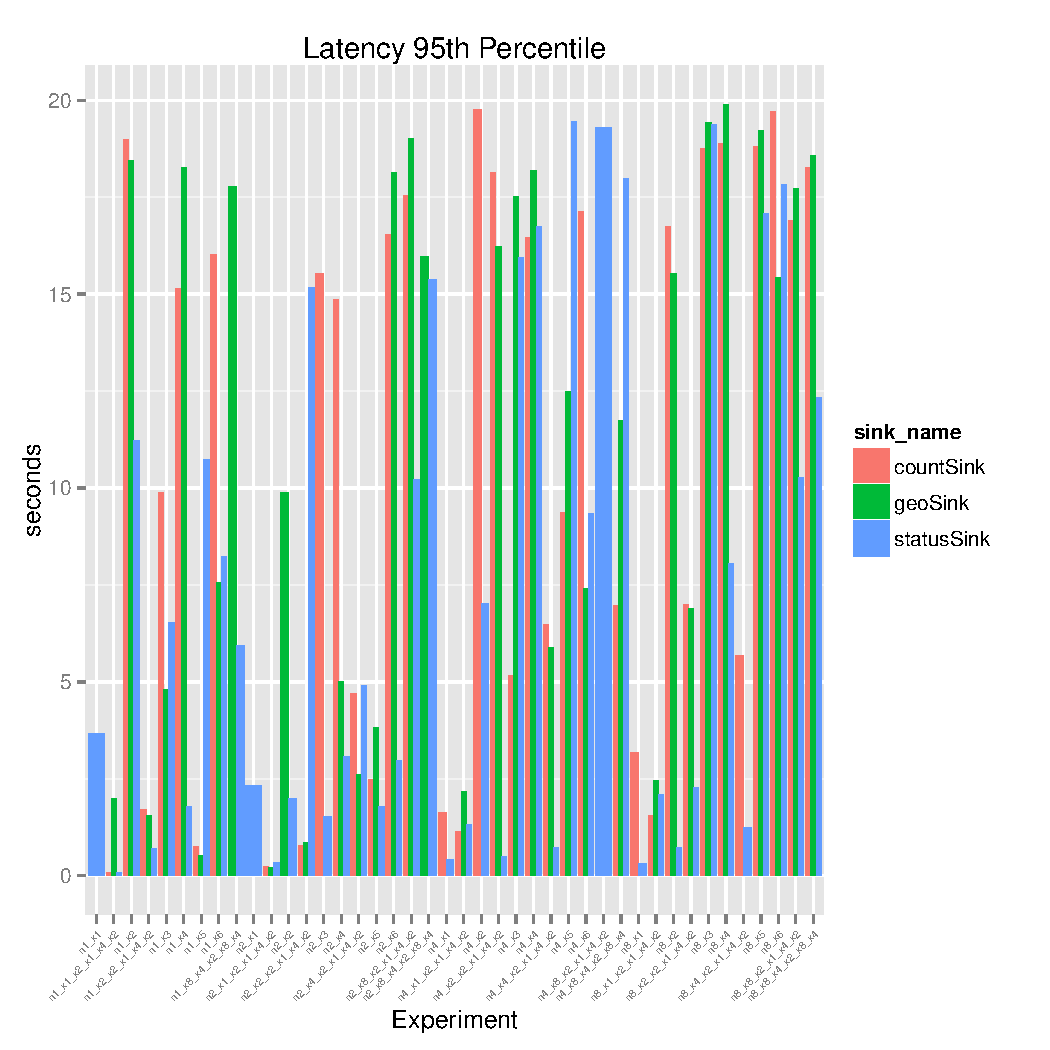
\includegraphics[width=.6\textwidth]{summaries/storm_logprocessing/best_latency.pdf}
	\caption{Storm Log Processing Best Latencies}
	\label{fig:storm_logprocessing_latency_best}
\end{figure}

The throughput average on Figure \ref{fig:storm_logprocessing_throughput} shows that a good configuration sometimes is better than adding more nodes to the application. At least 5 experiments with 4 nodes performed better than all but one experiment with 8 nodes, which is \textbf{n8\_x3}, with an average throughput of 8.6k tuples per second for \textit{geofinder}, \textit{geostats} and \textit{geo sink}, and around 10.4k tuples per second for the remaining operators.

\begin{figure}[H]
    \centering
	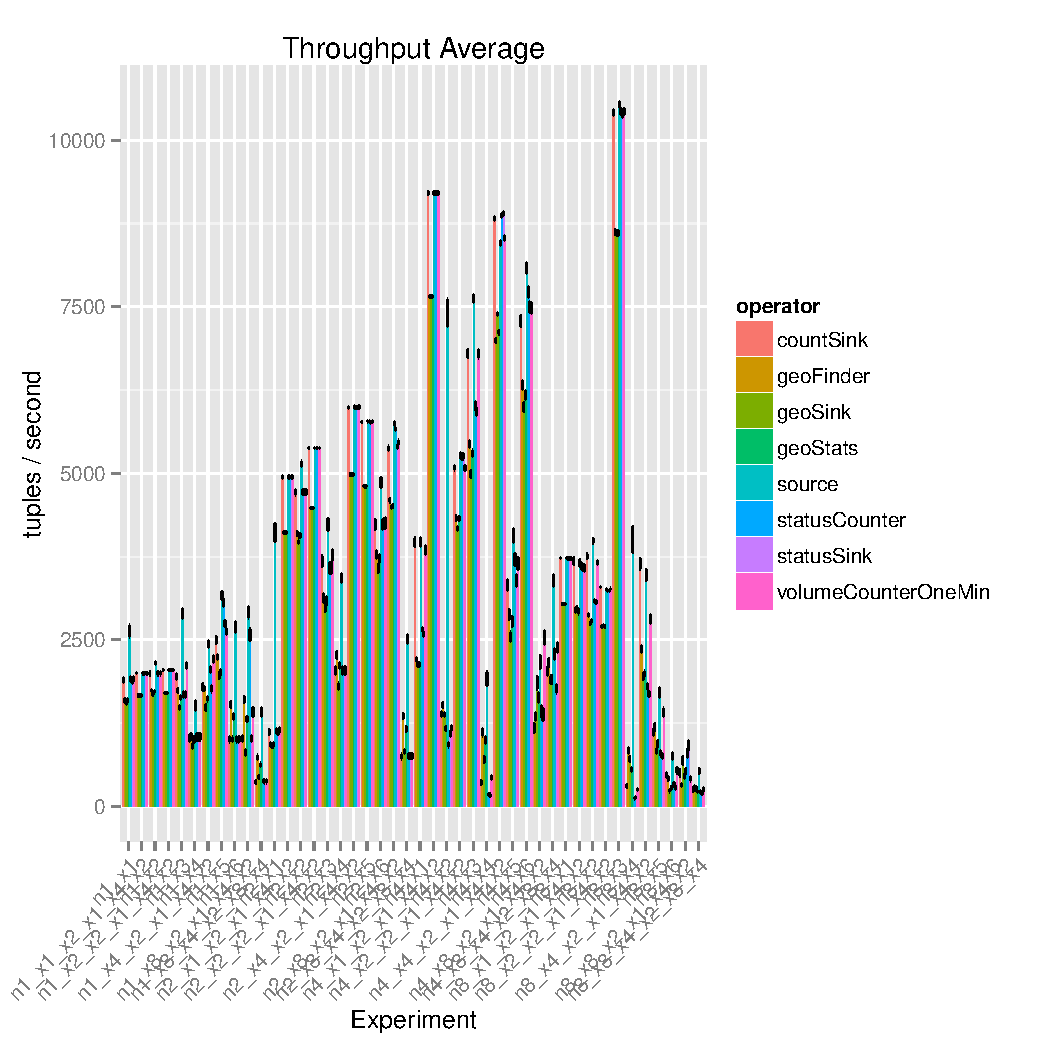
\includegraphics[width=.6\textwidth]{summaries/storm_logprocessing/full_throughput.pdf}
	\caption{Storm Log Processing Throughput}
	\label{fig:storm_logprocessing_throughput}
\end{figure}

Figure \ref{fig:storm_logprocessing_sink_throughput} shows only the throughput of the sink operators, i.e. the throughput of results.

\begin{figure}[H]
    \centering
	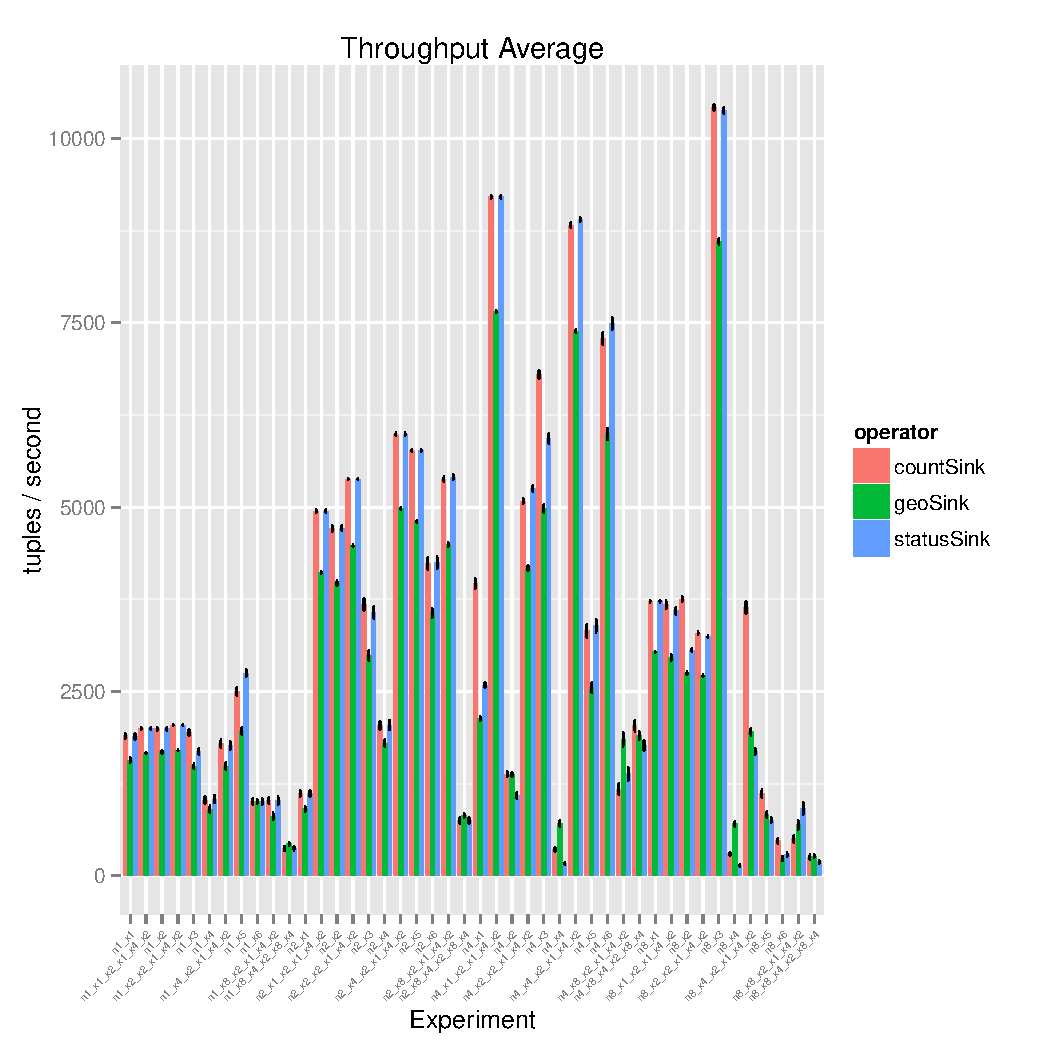
\includegraphics[width=.6\textwidth]{summaries/storm_logprocessing/sink_throughput.pdf}
	\caption{Storm Log Processing Sink Throughput}
	\label{fig:storm_logprocessing_sink_throughput}
\end{figure}

When looking at the network usage on Figure \ref{fig:storm_logprocessing_network} there is undoubtedly a resemblance with the throughput chart, with the most performant experiments were the ones that used more network, as they pushed more tuples downstream.

\begin{figure}[H]
    \centering
	\includegraphics[width=.6\textwidth]{summaries/storm_logprocessing/full_network.pdf}
	\caption{Storm Log Processing Network Usage}
	\label{fig:storm_logprocessing_network}
\end{figure}

The memory usage (Figure \ref{fig:storm_logprocessing_cpu_mem}) on the other hand decreased as more nodes were added. The CPU also had a similar trend, but looking more closely it is possible to notice that the highest CPU usages (above 50\%) are the ones that performed better on throughput.

\begin{figure}[H]
    \centering
	\includegraphics[width=.6\textwidth]{summaries/storm_logprocessing/full_cpu_mem.pdf}
	\caption{Storm Log Processing CPU and Memory Usage}
	\label{fig:storm_logprocessing_cpu_mem}
\end{figure}

Latencies on Spark, as seen on Figure \ref{fig:spark_logprocessing_latency}, ranged from 2.5 seconds to a little below 40 seconds. The best latencies occurred at experiment \textbf{n1\_x8\_x2\_x1\_x4\_x2} with 2.5 seconds for the \textit{volume counts sink}, 6.8 seconds for the \textit{country counts sink} and 9.3 seconds for the \textit{city counts sink}.

The chart suggests that for experiments within a number of nodes, increasing the number of source operators did improved the overall latency.

\begin{figure}[H]
    \centering
	\includegraphics[width=.6\textwidth]{summaries/spark_logprocessing/latency.pdf}
	\caption{Spark Log Processing Latencies}
	\label{fig:spark_logprocessing_latency}
\end{figure}

On the throughput for Spark (Figure \ref{fig:spark_logprocessing_throughput}) the best performant operator was the \textit{common log parser} (which is part of the \textit{source}), but in general thr throughput was worse than on Storm.

\begin{figure}[H]
    \centering
	\includegraphics[width=.6\textwidth]{summaries/spark_logprocessing/throughput.pdf}
	\caption{Spark Log Processing Throughput}
	\label{fig:spark_logprocessing_throughput}
\end{figure}

And if we look only at the throughput of the sinks results were much worse, with the \textit{city counts sink} operator showing the best results of those, but still very far from the numbers that Storm was able to deliver.

\begin{figure}[H]
    \centering
	\includegraphics[width=.6\textwidth]{summaries/spark_logprocessing/sink_throughput.pdf}
	\caption{Spark Log Processing Sink Throughput}
	\label{fig:spark_logprocessing_sink_throughput}
\end{figure}

The network usage on Figure \ref{fig:spark_logprocessing_network} shows a much lower traffic than the one of Storm experiments.

\begin{figure}[H]
    \centering
	\includegraphics[width=.6\textwidth]{summaries/spark_logprocessing/network.pdf}
	\caption{Spark Log Processing Network Usage}
	\label{fig:spark_logprocessing_network}
\end{figure}

And the CPU usage (Figure \ref{fig:spark_logprocessing_cpu_mem}) of the experiments show that it was being under used. Some of the experiments had a failure on the component that collected resource usage metrics.

\begin{figure}[H]
    \centering
	\includegraphics[width=.6\textwidth]{summaries/spark_logprocessing/cpu_mem.pdf}
	\caption{Spark Log Processing CPU and Memory Usage}
	\label{fig:spark_logprocessing_cpu_mem}
\end{figure}

The low resource usage by itself is not a bad sign, but together with the poor performance of the application, it shows that this application has a pattern of communication that is better suited for Storm, and it would have to be completely rethought for Spark architecture.

It is clear that for this application Storm did better in all aspects, and some experiments were able to deliver both high throughput as well as low latencies. It also evidenced that fine tuning the configurations of the experiment can achieve better results than simply increasing the number of nodes.

\begin{table}[H]
\tiny
\centering
\caption{Comparison of Log Processing results}
\label{table:log-processing-results}
\begin{tabular}{|l|l|l|l|l|l|l|l|}
\hline
Platform & Experiment                               & Throughput (volume)                      & Throughput (geo)                         & Throughput (status)                      & Latency (status)                         & Latency (geo)                            & Latency (volume)                         \\ \hline
Spark    &                                          & 1.93074324324324                         & 1.45959595959596                         & 9.58974358974359                         & 39320.4078552146                         & 32763.0934065934                         & 10448.3701592624                         \\ \cline{1-1} \cline{3-8} 
Storm    & \multirow{-2}{*}{n1\_x1\_x2\_x1\_x4\_x2} & \cellcolor[HTML]{67FD9A}1999.49816079874 & \cellcolor[HTML]{67FD9A}1665.76307531381 & \cellcolor[HTML]{67FD9A}1999.38707983193 & \cellcolor[HTML]{67FD9A}25.4692708333333 & \cellcolor[HTML]{67FD9A}210.478581979321 & \cellcolor[HTML]{67FD9A}3.29776158250911 \\ \hline
Spark    &                                          & 3.60240963855422                         & 3.80722891566265                         & 21.6270491803279                         & 18844.2364011935                         & 13988.976068038                          & 4872.89626207476                         \\ \cline{1-1} \cline{3-8} 
Storm    & \multirow{-2}{*}{n1\_x2\_x2\_x1\_x4\_x2} & \cellcolor[HTML]{67FD9A}2044.38279301746 & \cellcolor[HTML]{67FD9A}1700.90633437175 & \cellcolor[HTML]{67FD9A}2043.32107995846 & \cellcolor[HTML]{67FD9A}1118.59902597403 & \cellcolor[HTML]{67FD9A}726.931209415584 & \cellcolor[HTML]{67FD9A}307.97442662878  \\ \hline
Spark    &                                          & 4.04347826086957                         & 5.6231884057971                          & 27.0359712230216                         & \cellcolor[HTML]{67FD9A}11957.5660586572 & \cellcolor[HTML]{67FD9A}9016.64420289855 & \cellcolor[HTML]{67FD9A}3582.41756393001 \\ \cline{1-1} \cline{3-8} 
Storm    & \multirow{-2}{*}{n1\_x4\_x2\_x1\_x4\_x2} & \cellcolor[HTML]{67FD9A}1792.96754250386 & \cellcolor[HTML]{67FD9A}1484.9984399376  & \cellcolor[HTML]{67FD9A}1767.88682170543 & 111913.900306748                         & 183408.307573416                         & 102437.234662577                         \\ \hline
Spark    &                                          & 5.07407407407407                         & 7.5875                                   & 31.8780487804878                         & \cellcolor[HTML]{67FD9A}9396.85105597401 & \cellcolor[HTML]{67FD9A}6860.51700888753 & \cellcolor[HTML]{67FD9A}2569.37347215935 \\ \cline{1-1} \cline{3-8} 
Storm    & \multirow{-2}{*}{n1\_x8\_x2\_x1\_x4\_x2} & \cellcolor[HTML]{67FD9A}1023.67365269461 & \cellcolor[HTML]{67FD9A}808.489795918367 & \cellcolor[HTML]{67FD9A}1020.39150943396 & 37971.9610849057                         & 116636.56462585                          & 59924.9356643357                         \\ \hline
Spark    &                                          & 1.80769230769231                         & 2.08395061728395                         & 12.1571072319202                         & 25914.887547413                          & 23388.7110609481                         & \cellcolor[HTML]{67FD9A}8541.72202998847 \\ \cline{1-1} \cline{3-8} 
Storm    & \multirow{-2}{*}{n2\_x1\_x2\_x1\_x4\_x2} & \cellcolor[HTML]{67FD9A}4942.92461252325 & \cellcolor[HTML]{67FD9A}4115.75576493925 & \cellcolor[HTML]{67FD9A}4942.86265030371 & \cellcolor[HTML]{67FD9A}236.293664383562 & \cellcolor[HTML]{67FD9A}192.08291549468  & 20281.1640988017                         \\ \hline
Spark    &                                          & 3.10795454545455                         & 4.75852272727273                         & 25.5498575498575                         & \cellcolor[HTML]{67FD9A}12859.9195729352 & 10726.1025669768                         & 4156.42327150084                         \\ \cline{1-1} \cline{3-8} 
Storm    & \multirow{-2}{*}{n2\_x2\_x2\_x1\_x4\_x2} & \cellcolor[HTML]{67FD9A}5381.4324017821  & \cellcolor[HTML]{67FD9A}4479.3023331173  & \cellcolor[HTML]{67FD9A}5381.44475048607 & 24743.644184007                          & \cellcolor[HTML]{67FD9A}362.858555254345 & \cellcolor[HTML]{67FD9A}77.1451008530655 \\ \hline
Spark    &                                          & 4.09375                                  & 7.04484304932735                         & 35.6547085201794                         & \cellcolor[HTML]{67FD9A}10878.4345621221 & 7308.70540796964                         & \cellcolor[HTML]{67FD9A}2965.66518757564 \\ \cline{1-1} \cline{3-8} 
Storm    & \multirow{-2}{*}{n2\_x4\_x2\_x1\_x4\_x2} & \cellcolor[HTML]{67FD9A}5989.15232249965 & \cellcolor[HTML]{67FD9A}4983.80786391523 & \cellcolor[HTML]{67FD9A}5988.9188397713  & 3802019.8191937                          & \cellcolor[HTML]{67FD9A}1029.07190340524 & 4906.24301221167                         \\ \hline
Spark    &                                          & 4.10795454545455                         & 7.17241379310345                         & 35.4034090909091                         & \cellcolor[HTML]{67FD9A}9320.77174347363 & \cellcolor[HTML]{67FD9A}7221.83235207536 & \cellcolor[HTML]{67FD9A}3017.44391227628 \\ \cline{1-1} \cline{3-8} 
Storm    & \multirow{-2}{*}{n2\_x8\_x2\_x1\_x4\_x2} & \cellcolor[HTML]{67FD9A}5376.56247689464 & \cellcolor[HTML]{67FD9A}4493.01784386617 & \cellcolor[HTML]{67FD9A}5406.84413407821 & 15828.41322616                           & 18999.1075740944                         & 7807.59147129407                         \\ \hline
Spark    &                                          & 0.892212480660134                        & 1.80051948051948                         & 11.2502651113468                         & 32319.1317641322                         & 28642.2336169982                         & 9776.59511012752                         \\ \cline{1-1} \cline{3-8} 
Storm    & \multirow{-2}{*}{n4\_x1\_x2\_x1\_x4\_x2} & \cellcolor[HTML]{67FD9A}9208.31336622034 & \cellcolor[HTML]{67FD9A}7650.84866515306 & \cellcolor[HTML]{67FD9A}9208.85618100681 & \cellcolor[HTML]{67FD9A}1864.90594402899 & \cellcolor[HTML]{67FD9A}872.857142857143 & \cellcolor[HTML]{67FD9A}629.973012568432 \\ \hline
Spark    &                                          & 1.70675830469645                         & 3.9495990836197                          & 22.0826636050517                         & 16595.0432314056                         & 13604.8738597043                         & \cellcolor[HTML]{67FD9A}5243.91422227416 \\ \cline{1-1} \cline{3-8} 
Storm    & \multirow{-2}{*}{n4\_x2\_x2\_x1\_x4\_x2} & \cellcolor[HTML]{67FD9A}5083.0700677392  & \cellcolor[HTML]{67FD9A}4171.86825329367 & \cellcolor[HTML]{67FD9A}5254.0934856176  & \cellcolor[HTML]{67FD9A}16218.1368464903 & \cellcolor[HTML]{67FD9A}499.782032705444 & 27854.4848736013                         \\ \hline
Spark    &                                          & 2.33732876712329                         & 5.01384083044983                         & 27.2170138888889                         & 12541.8374106345                         & 9825.25911136464                         & \cellcolor[HTML]{67FD9A}3721.20620607347 \\ \cline{1-1} \cline{3-8} 
Storm    & \multirow{-2}{*}{n4\_x4\_x2\_x1\_x4\_x2} & \cellcolor[HTML]{67FD9A}8825.00245003224 & \cellcolor[HTML]{67FD9A}7387.03734815198 & \cellcolor[HTML]{67FD9A}8897.76182476092 & \cellcolor[HTML]{67FD9A}3284.87131158196 & \cellcolor[HTML]{67FD9A}382.610634425377 & 6472.52366135097                         \\ \hline
Spark    &                                          & 3.09714285714286                         & 6.37677053824363                         & 32.752808988764                          & \cellcolor[HTML]{67FD9A}9469.56498604163 & \cellcolor[HTML]{67FD9A}7030.42323685283 & \cellcolor[HTML]{67FD9A}2720.64934032745 \\ \cline{1-1} \cline{3-8} 
Storm    & \multirow{-2}{*}{n4\_x8\_x2\_x1\_x4\_x2} & \cellcolor[HTML]{67FD9A}1176.65731814198 & \cellcolor[HTML]{67FD9A}1852.23063683305 & \cellcolor[HTML]{67FD9A}1382.53546712803 & 34237.3238312429                         & 19055.1666666667                         & 44461.5660592255                         \\ \hline
Spark    &                                          & 0.757650695517774                        & 2.18836993504485                         & 15.2482225656878                         & \cellcolor[HTML]{67FD9A}31428.8288714711 & 28101.5933059909                         & 9812.29875742842                         \\ \cline{1-1} \cline{3-8} 
Storm    & \multirow{-2}{*}{n8\_x1\_x2\_x1\_x4\_x2} & \cellcolor[HTML]{67FD9A}3677.28770595691 & \cellcolor[HTML]{67FD9A}2962.79001751313 & \cellcolor[HTML]{67FD9A}3592.05783516095 & 318009.129168872                         & \cellcolor[HTML]{67FD9A}1262.60083960119 & \cellcolor[HTML]{67FD9A}771.29125867901  \\ \hline
Spark    &                                          & 1.09874759152216                         & 3.16180758017493                         & 21.2980068060282                         & 21628.3989673364                         & 18268.3719072365                         & 6969.39617018106                         \\ \cline{1-1} \cline{3-8} 
Storm    & \multirow{-2}{*}{n8\_x2\_x2\_x1\_x4\_x2} & \cellcolor[HTML]{67FD9A}3293.16665384319 & \cellcolor[HTML]{67FD9A}2713.46872139152 & \cellcolor[HTML]{67FD9A}3240.02567418508 & \cellcolor[HTML]{67FD9A}4223.38037608671 & \cellcolor[HTML]{67FD9A}2271.51888335298 & \cellcolor[HTML]{67FD9A}4737.74523029485 \\ \hline
Spark    &                                          & 1.81303116147309                         & 5.28248587570621                         & 32.0189393939394                         & \cellcolor[HTML]{67FD9A}12935.8142177238 & 10041.5958139964                         & \cellcolor[HTML]{67FD9A}3977.96003946719 \\ \cline{1-1} \cline{3-8} 
Storm    & \multirow{-2}{*}{n8\_x4\_x2\_x1\_x4\_x2} & \cellcolor[HTML]{67FD9A}3643.99029462738 & \cellcolor[HTML]{67FD9A}1955.13460533194 & \cellcolor[HTML]{67FD9A}1683.90825688073 & 51693.4150064683                         & \cellcolor[HTML]{67FD9A}569.368954165612 & 778856.216830933                         \\ \hline
Spark    &                                          & 2.32819722650231                         & 6.72617246596067                         & 40.58114374034                           & \cellcolor[HTML]{67FD9A}10026.1596979203 & 7610.76036029217                         & \cellcolor[HTML]{67FD9A}2867.36524861277 \\ \cline{1-1} \cline{3-8} 
Storm    & \multirow{-2}{*}{n8\_x8\_x2\_x1\_x4\_x2} & \cellcolor[HTML]{67FD9A}500.99245852187  & \cellcolor[HTML]{67FD9A}690.335548172758 & \cellcolor[HTML]{67FD9A}912.130870953032 & 25391.7222929936                         & \cellcolor[HTML]{67FD9A}3546.92970521542 & 38895.4339222615                         \\ \hline
\end{tabular}
\end{table}

On Table \ref{table:log-processing-results} it is possible to see that Storm did better on all throughput results, while on latency results were more balanced, with Storm doing better on 25 out of 48 results, very close to Spark.


\section{Traffic Monitoring}

For the Traffic Monitoring application, 40 different configurations were executed on Storm and a subset of 3 configurations on Spark.

Each configuration is identified by \textbf{n\textit{N}}\_\textbf{x\textit{Source}}\_\textbf{x\textit{MapMatcher}}\_\textbf{x\textit{SpeedCalculator}}\_\textbf{x\textit{Sink}} which is the number of nodes and the number of instances of each operator. If only one \textbf{x\textit{X}} is defined, it means all operators have the same number of instances.

As expected, some experiments show very high latencies (Figure \ref{fig:storm_trafficmonitoring_latency}), with 6 experiments having the 95th percentile of latency above 10 thousand seconds.

\begin{figure}[H]
    \centering
	\includegraphics[width=.6\textwidth]{summaries/storm_trafficmonitoring/full_latency.pdf}
	\caption{Storm Traffic Monitoring Latencies}
	\label{fig:storm_trafficmonitoring_latency}
\end{figure}

Looking at the best performers on latency there are 15 experiments with results below 20 seconds of latency.

\begin{figure}[H]
    \centering
	\includegraphics[width=.6\textwidth]{summaries/storm_trafficmonitoring/best_latency.pdf}
	\caption{Storm Traffic Monitoring Best Latencies}
	\label{fig:storm_trafficmonitoring_latency_best}
\end{figure}

The throughput average on Figure \ref{fig:storm_trafficmonitoring_throughput} shows that only the source operator is able to deliver a high throughput.

\begin{figure}[H]
    \centering
	\includegraphics[width=.6\textwidth]{summaries/storm_trafficmonitoring/full_throughput.pdf}
	\caption{Storm Traffic Monitoring Throughput}
	\label{fig:storm_trafficmonitoring_throughput}
\end{figure}

When looking at the other operators without the source on Figure \ref{fig:storm_trafficmonitoring_throughput2} it is possible to observer that the other operators deliver a very low throughput, which is something expected for this application, as it is not always able to match a coordinate to a street in a map.

The experiment with the best results was \textbf{n8\_x4} with 35 tuples per second for the three operators.

\begin{figure}[H]
    \centering
	\includegraphics[width=.6\textwidth]{summaries/storm_trafficmonitoring/throughput2.pdf}
	\caption{Storm Traffic Monitoring Throughput without the Source Operator}
	\label{fig:storm_trafficmonitoring_throughput2}
\end{figure}

On the network usage chart of Figure \ref{fig:storm_trafficmonitoring_network}, the highest usage was that of experiment \textbf{n8\_x4\_x2\_x2}, which suggests that some arrangements of number of operators might lead to more communication among nodes without necessarily increasing the  performance. In fact, it could actually decrease the performance as more time is spent doing communication.

\begin{figure}[H]
    \centering
	\includegraphics[width=.6\textwidth]{summaries/storm_trafficmonitoring/full_network.pdf}
	\caption{Storm Traffic Monitoring Network Usage}
	\label{fig:storm_trafficmonitoring_network}
\end{figure}

The CPU usage on Figure \ref{fig:storm_trafficmonitoring_cpu_mem} also shows a trend for each node size, with the usage increasing as the number of instances of each operator increases. While the memory seemed more stable, with a few experiments peaking above the 75\% line.

\begin{figure}[H]
    \centering
	\includegraphics[width=.6\textwidth]{summaries/storm_trafficmonitoring/full_cpu_mem.pdf}
	\caption{Storm Traffic Monitoring CPU and Memory Usage}
	\label{fig:storm_trafficmonitoring_cpu_mem}
\end{figure}


The latencies on Spark (Figure \ref{fig:spark_trafficmonitoring_latency}) were extremely high, all of them going over 20 thousand seconds.

\begin{figure}[H]
    \centering
	\includegraphics[width=.6\textwidth]{summaries/spark_trafficmonitoring/latency.pdf}
	\caption{Spark Traffic Monitoring Latencies}
	\label{fig:spark_trafficmonitoring_latency}
\end{figure}

The throughput on Figure \ref{fig:spark_trafficmonitoring_throughput} shows that Spark did a little better on the \textit{MapMatcher} operator, while on the \textit{SpeedCalculator} and \textit{Sink} the performance was under 10 tuples per second. A comparison of the experiments \textbf{n1\_x4\_x2\_x2}, \textbf{n4\_x2\_x2\_x2} and \textbf{n4\_x8\_x2\_x2} between Spark and Storm also confirms that at the \textit{sink} operator Storm performed a little better than Spark, but the difference was very small.

\begin{figure}[H]
    \centering
	\includegraphics[width=.6\textwidth]{summaries/spark_trafficmonitoring/throughput.pdf}
	\caption{Spark Traffic Monitoring Throughput}
	\label{fig:spark_trafficmonitoring_throughput}
\end{figure}

The network usage of the experiments on Spark, seen on Figure \ref{fig:spark_trafficmonitoring_network} shows very little traffic happening between the nodes, something compatible with the level of throughput of the application.

\begin{figure}[H]
    \centering
	\includegraphics[width=.6\textwidth]{summaries/spark_trafficmonitoring/network.pdf}
	\caption{Spark Traffic Monitoring Network Usage}
	\label{fig:spark_trafficmonitoring_network}
\end{figure}

The CPU and memory usage (Figure \ref{fig:spark_trafficmonitoring_cpu_mem}) are much higher for a single node, than for 4 nodes.

\begin{figure}[H]
    \centering
	\includegraphics[width=.6\textwidth]{summaries/spark_trafficmonitoring/cpu_mem.pdf}
	\caption{Spark Traffic Monitoring CPU and Memory Usage}
	\label{fig:spark_trafficmonitoring_cpu_mem}
\end{figure}

The results show that this application is not very CPU and network intensive, and it also shows that both Spark and Storm showed similar performance results.

\begin{table}[H]
\tiny
\centering
\caption{Comparison of Traffic Monitoring results}
\label{table:traffic-monitoring-results}
\begin{tabular}{|l|l|l|l|l}
\cline{1-4}
Platform & Experiment                       & Throughput                               & Latency                                  &  \\ \cline{1-4}
Spark    &                                  & 9.196423997131                           & 43616859.3358191                         &  \\ \cline{1-1} \cline{3-4}
Storm    & \multirow{-2}{*}{n1\_x4\_x2\_x2} & \cellcolor[HTML]{67FD9A}15.8215599927611 & \cellcolor[HTML]{67FD9A}12213831.6247981 &  \\ \cline{1-4}
Spark    &                                  & 5.80584934167926                         & 35302215.9149239                         &  \\ \cline{1-1} \cline{3-4}
Storm    & \multirow{-2}{*}{n4\_x2\_x2\_x2} & \cellcolor[HTML]{67FD9A}10.17202268431   & \cellcolor[HTML]{67FD9A}504721.903280067 &  \\ \cline{1-4}
Spark    &                                  & 7.2561553030303                          & 21290498.8742954                         &  \\ \cline{1-1} \cline{3-4}
Storm    & \multirow{-2}{*}{n4\_x8\_x2\_x2} & \cellcolor[HTML]{67FD9A}9.4453125        & \cellcolor[HTML]{67FD9A}109004.985135135 &  \\ \cline{1-4}
\end{tabular}
\end{table}

On Table \ref{table:traffic-monitoring-results} results show that Storm did better on all experiments.


\section{Analysis of the Results}

Storm did better generally than Spark on throughput, but on latency results were more balanced between the two platforms.

Regarding resource usage:
- if spark better than storm, how was the resource usage?
- if storm better than spark, how was the resource usage?

Analysis of best configurations for each number of nodes. (table perhaps).

% TODO:
% improve the conclusion

% revise all chart images, remove duplicate error bars

% include those new references: stream processing benchmark from 2016 on
% StreamBench: uses wordcount, click stream app and kmeans \citep{wang2016stream}
% but it compares storm, spark and flink
% mine has more applications

% RIoTBench: \citep{shukla2016benchmarking} and \citep{shukla2017riotbench}
% Storm on Azure

% Yahoo Stream Benchmark? 

% Flink Streaming

% Highlight on the chart the best config for each number of nodes.

% -----------------------------------------------------------------------------
\chapter{Conclusion}
\label{chapter:conclusion}

Event stream processing is an emerging set of technologies that already encompasses several application areas and system implementations. In this work we introduced a benchmark suite designed specifically to evaluate SPSs, with a wide variety of applications, a well defined set of metrics for the correct interpretation of results and a methodology to guarantee the quality of the results.

The design and development a basic framework to help the execution and collection of results proved essential for this kind of experiments, as a lot of data is generated and it needs to be processed, summarized and plotted into charts in order for a better understanding of the results obtained.

The results from Chapter \ref{chapter:results} show that the proposed framework provides the necessary tools to properly execute, collect and compare stream processing frameworks. Specifically, the results showed that Storm has a better performance than Spark when it comes to throughput, even though Spark uses micro-batches. But on latency the results showed more balanced results between Storm and Spark.

In the end, the configuration of the number of instances of each operator was key to a good performance. And this work showed that knowing beforehand the selectivity of each operator was helpful in the selection of good configurations.

As opposed to previous works, we have defined a set of applications from several areas, ranging different types of workloads, communication patterns and inputs from real world. We have also defined a framework in order to help the development and benchmarking of stream applications without the necessity of rewriting the application for each platform.

In the future, the comparison of SPSs could be expanded to encompass more platforms as well as the whole set of applications defined in the benchmark. In addition, a more extensive analysis of the metrics could have been done, which could lead to a new set of metrics derived from the basic metrics defined in this benchmark.

Future comparisons could also try to introduce failures to analyse the resilience of these systems, as well as the tuple loss in order to know how much load a system can take without loosing information.

The stream processing landscape is full of challenges and it has plentiful of new platforms, thus having a benchmark capable of evaluating them in meaningful ways is going to be very useful.


\bibliographystyle{abntex2-alf}
\bibliography{bibliography}

\end{document}
